% Options for packages loaded elsewhere
\PassOptionsToPackage{unicode}{hyperref}
\PassOptionsToPackage{hyphens}{url}
%
\documentclass[
]{article}
\usepackage{amsmath,amssymb}
\usepackage{lmodern}
\usepackage{iftex}
\ifPDFTeX
  \usepackage[T1]{fontenc}
  \usepackage[utf8]{inputenc}
  \usepackage{textcomp} % provide euro and other symbols
\else % if luatex or xetex
  \usepackage{unicode-math}
  \defaultfontfeatures{Scale=MatchLowercase}
  \defaultfontfeatures[\rmfamily]{Ligatures=TeX,Scale=1}
\fi
% Use upquote if available, for straight quotes in verbatim environments
\IfFileExists{upquote.sty}{\usepackage{upquote}}{}
\IfFileExists{microtype.sty}{% use microtype if available
  \usepackage[]{microtype}
  \UseMicrotypeSet[protrusion]{basicmath} % disable protrusion for tt fonts
}{}
\makeatletter
\@ifundefined{KOMAClassName}{% if non-KOMA class
  \IfFileExists{parskip.sty}{%
    \usepackage{parskip}
  }{% else
    \setlength{\parindent}{0pt}
    \setlength{\parskip}{6pt plus 2pt minus 1pt}}
}{% if KOMA class
  \KOMAoptions{parskip=half}}
\makeatother
\usepackage{xcolor}
\usepackage[margin=1in]{geometry}
\usepackage{color}
\usepackage{fancyvrb}
\newcommand{\VerbBar}{|}
\newcommand{\VERB}{\Verb[commandchars=\\\{\}]}
\DefineVerbatimEnvironment{Highlighting}{Verbatim}{commandchars=\\\{\}}
% Add ',fontsize=\small' for more characters per line
\usepackage{framed}
\definecolor{shadecolor}{RGB}{248,248,248}
\newenvironment{Shaded}{\begin{snugshade}}{\end{snugshade}}
\newcommand{\AlertTok}[1]{\textcolor[rgb]{0.94,0.16,0.16}{#1}}
\newcommand{\AnnotationTok}[1]{\textcolor[rgb]{0.56,0.35,0.01}{\textbf{\textit{#1}}}}
\newcommand{\AttributeTok}[1]{\textcolor[rgb]{0.77,0.63,0.00}{#1}}
\newcommand{\BaseNTok}[1]{\textcolor[rgb]{0.00,0.00,0.81}{#1}}
\newcommand{\BuiltInTok}[1]{#1}
\newcommand{\CharTok}[1]{\textcolor[rgb]{0.31,0.60,0.02}{#1}}
\newcommand{\CommentTok}[1]{\textcolor[rgb]{0.56,0.35,0.01}{\textit{#1}}}
\newcommand{\CommentVarTok}[1]{\textcolor[rgb]{0.56,0.35,0.01}{\textbf{\textit{#1}}}}
\newcommand{\ConstantTok}[1]{\textcolor[rgb]{0.00,0.00,0.00}{#1}}
\newcommand{\ControlFlowTok}[1]{\textcolor[rgb]{0.13,0.29,0.53}{\textbf{#1}}}
\newcommand{\DataTypeTok}[1]{\textcolor[rgb]{0.13,0.29,0.53}{#1}}
\newcommand{\DecValTok}[1]{\textcolor[rgb]{0.00,0.00,0.81}{#1}}
\newcommand{\DocumentationTok}[1]{\textcolor[rgb]{0.56,0.35,0.01}{\textbf{\textit{#1}}}}
\newcommand{\ErrorTok}[1]{\textcolor[rgb]{0.64,0.00,0.00}{\textbf{#1}}}
\newcommand{\ExtensionTok}[1]{#1}
\newcommand{\FloatTok}[1]{\textcolor[rgb]{0.00,0.00,0.81}{#1}}
\newcommand{\FunctionTok}[1]{\textcolor[rgb]{0.00,0.00,0.00}{#1}}
\newcommand{\ImportTok}[1]{#1}
\newcommand{\InformationTok}[1]{\textcolor[rgb]{0.56,0.35,0.01}{\textbf{\textit{#1}}}}
\newcommand{\KeywordTok}[1]{\textcolor[rgb]{0.13,0.29,0.53}{\textbf{#1}}}
\newcommand{\NormalTok}[1]{#1}
\newcommand{\OperatorTok}[1]{\textcolor[rgb]{0.81,0.36,0.00}{\textbf{#1}}}
\newcommand{\OtherTok}[1]{\textcolor[rgb]{0.56,0.35,0.01}{#1}}
\newcommand{\PreprocessorTok}[1]{\textcolor[rgb]{0.56,0.35,0.01}{\textit{#1}}}
\newcommand{\RegionMarkerTok}[1]{#1}
\newcommand{\SpecialCharTok}[1]{\textcolor[rgb]{0.00,0.00,0.00}{#1}}
\newcommand{\SpecialStringTok}[1]{\textcolor[rgb]{0.31,0.60,0.02}{#1}}
\newcommand{\StringTok}[1]{\textcolor[rgb]{0.31,0.60,0.02}{#1}}
\newcommand{\VariableTok}[1]{\textcolor[rgb]{0.00,0.00,0.00}{#1}}
\newcommand{\VerbatimStringTok}[1]{\textcolor[rgb]{0.31,0.60,0.02}{#1}}
\newcommand{\WarningTok}[1]{\textcolor[rgb]{0.56,0.35,0.01}{\textbf{\textit{#1}}}}
\usepackage{graphicx}
\makeatletter
\def\maxwidth{\ifdim\Gin@nat@width>\linewidth\linewidth\else\Gin@nat@width\fi}
\def\maxheight{\ifdim\Gin@nat@height>\textheight\textheight\else\Gin@nat@height\fi}
\makeatother
% Scale images if necessary, so that they will not overflow the page
% margins by default, and it is still possible to overwrite the defaults
% using explicit options in \includegraphics[width, height, ...]{}
\setkeys{Gin}{width=\maxwidth,height=\maxheight,keepaspectratio}
% Set default figure placement to htbp
\makeatletter
\def\fps@figure{htbp}
\makeatother
\setlength{\emergencystretch}{3em} % prevent overfull lines
\providecommand{\tightlist}{%
  \setlength{\itemsep}{0pt}\setlength{\parskip}{0pt}}
\setcounter{secnumdepth}{-\maxdimen} % remove section numbering
\ifLuaTeX
  \usepackage{selnolig}  % disable illegal ligatures
\fi
\IfFileExists{bookmark.sty}{\usepackage{bookmark}}{\usepackage{hyperref}}
\IfFileExists{xurl.sty}{\usepackage{xurl}}{} % add URL line breaks if available
\urlstyle{same} % disable monospaced font for URLs
\hypersetup{
  pdftitle={Infection Intensity Data Analysis},
  pdfauthor={Lindsay E. Martin},
  hidelinks,
  pdfcreator={LaTeX via pandoc}}

\title{Infection Intensity Data Analysis}
\author{Lindsay E. Martin}
\date{2022-08-10}

\begin{document}
\maketitle

\begin{verbatim}
## [1] "C:/Users/linzm/OneDrive - Vanderbilt/Hillyer_Lab/Infection_Intensity"
\end{verbatim}

\begin{verbatim}
## 
## Attaching package: 'dplyr'
\end{verbatim}

\begin{verbatim}
## The following objects are masked from 'package:stats':
## 
##     filter, lag
\end{verbatim}

\begin{verbatim}
## The following objects are masked from 'package:base':
## 
##     intersect, setdiff, setequal, union
\end{verbatim}

\begin{verbatim}
## -- Attaching packages --------------------------------------- tidyverse 1.3.2 --
## v tibble  3.1.8     v purrr   0.3.4
## v tidyr   1.2.0     v stringr 1.4.0
## v readr   2.1.2     v forcats 0.5.1
## -- Conflicts ------------------------------------------ tidyverse_conflicts() --
## x dplyr::filter() masks stats::filter()
## x dplyr::lag()    masks stats::lag()
## 
## Attaching package: 'rstatix'
## 
## 
## The following object is masked from 'package:stats':
## 
##     filter
## 
## 
## Loading required package: carData
## 
## 
## Attaching package: 'car'
## 
## 
## The following object is masked from 'package:purrr':
## 
##     some
## 
## 
## The following object is masked from 'package:dplyr':
## 
##     recode
## 
## 
## 
## Attaching package: 'MASS'
## 
## 
## The following object is masked from 'package:rstatix':
## 
##     select
## 
## 
## The following object is masked from 'package:dplyr':
## 
##     select
## 
## 
## Loading required package: pscl
## 
## Classes and Methods for R developed in the
## Political Science Computational Laboratory
## Department of Political Science
## Stanford University
## Simon Jackman
## hurdle and zeroinfl functions by Achim Zeileis
## 
## Loading required package: zoo
## 
## 
## Attaching package: 'zoo'
## 
## 
## The following objects are masked from 'package:base':
## 
##     as.Date, as.Date.numeric
## 
## 
## Loading required package: foreign
## 
## Loading required package: fitdistrplus
## 
## Loading required package: survival
\end{verbatim}

\begin{verbatim}
## tibble [696 x 7] (S3: tbl_df/tbl/data.frame)
##  $ Trial          : num [1:696] 1 1 1 1 1 1 1 1 1 2 ...
##  $ ID             : num [1:696] 1 2 3 4 5 6 7 8 9 1 ...
##  $ Temperature    : num [1:696] 27 27 27 27 27 27 27 27 27 27 ...
##  $ Age            : num [1:696] 1 1 1 1 1 1 1 1 1 1 ...
##  $ CFUs           : num [1:696] 26000 7500 14500 28500 157500 ...
##  $ Block          : Factor w/ 20 levels "1","2","3","4",..: 1 1 1 1 1 1 1 1 1 2 ...
##  $ Infectious_Dose: num [1:696] 25254 25254 25254 25254 25254 ...
\end{verbatim}

\hypertarget{exploring-the-data}{%
\subsection{Exploring the Data}\label{exploring-the-data}}

First, we will plot the data to see what it looks like for each
temperature-age combination.

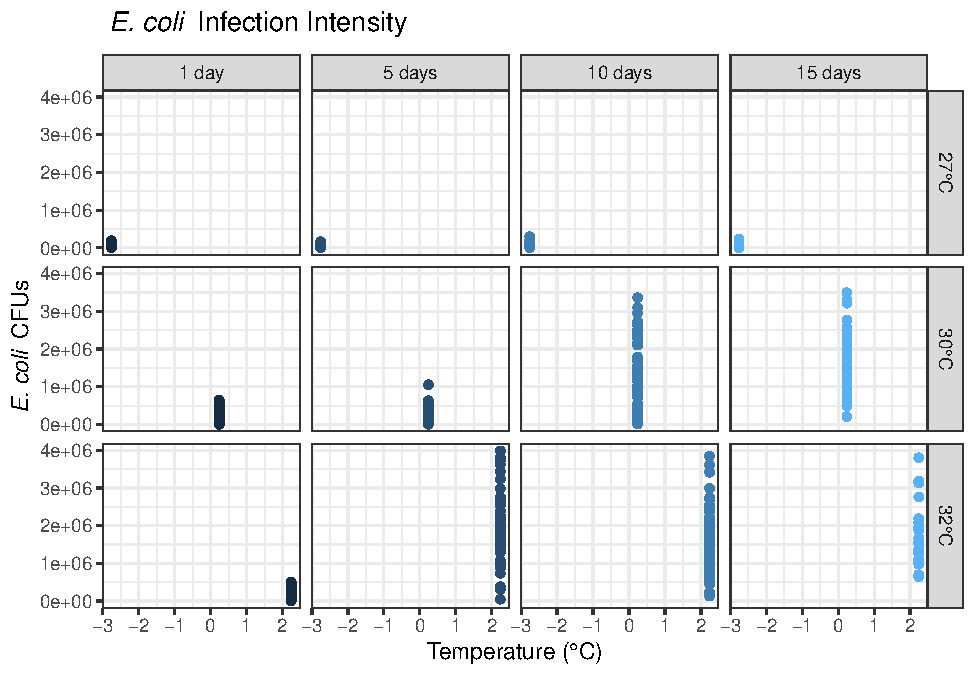
\includegraphics{Ecoli_infection_intensity_JSdata_Rmarkdownfile-081022_files/figure-latex/unnamed-chunk-1-1.pdf}
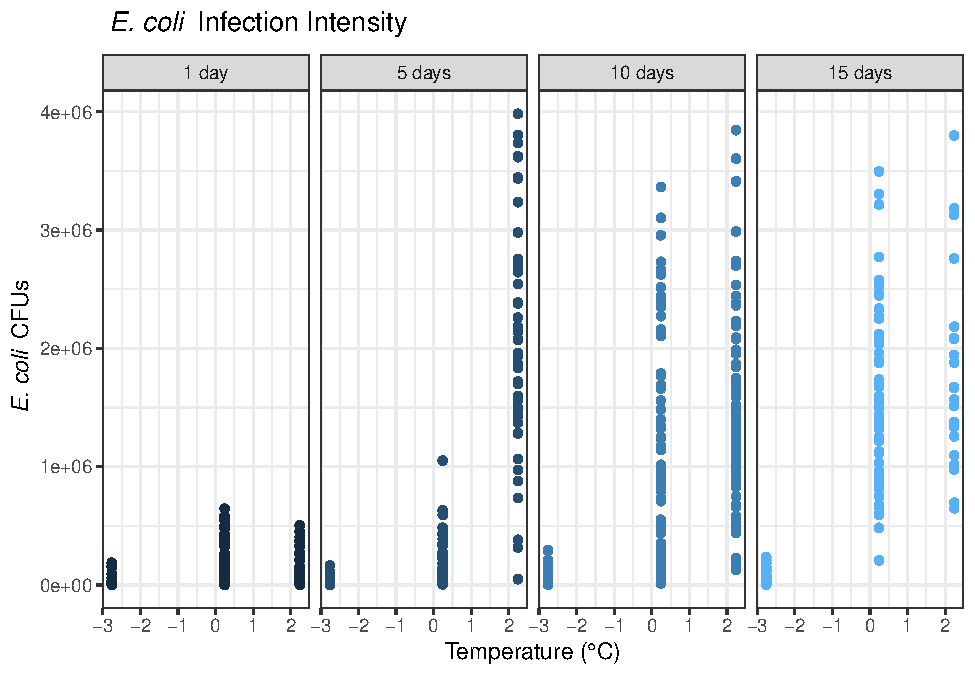
\includegraphics{Ecoli_infection_intensity_JSdata_Rmarkdownfile-081022_files/figure-latex/unnamed-chunk-1-2.pdf}
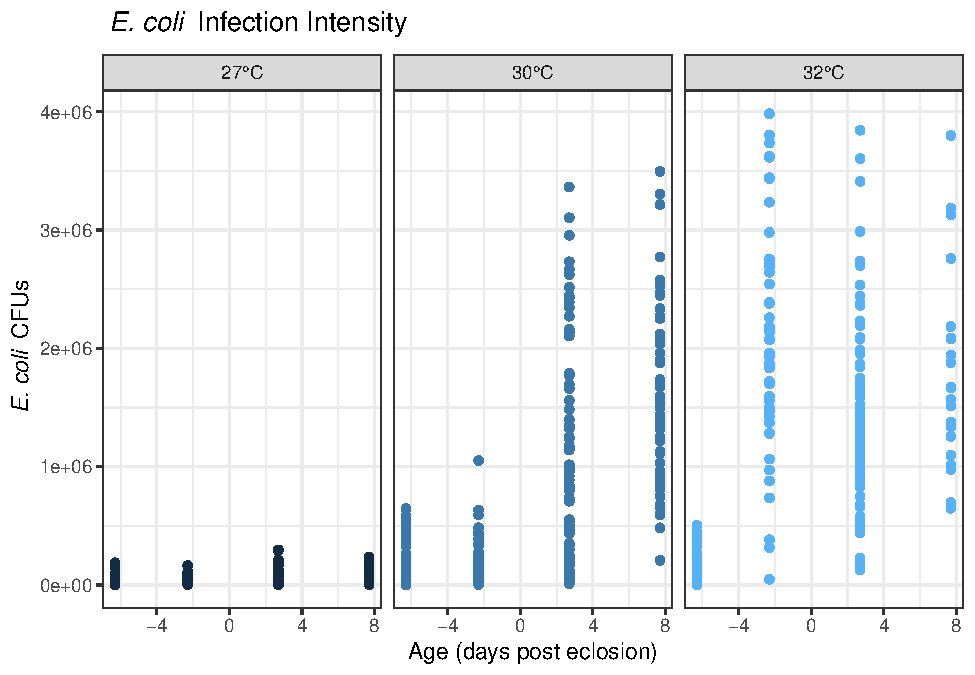
\includegraphics{Ecoli_infection_intensity_JSdata_Rmarkdownfile-081022_files/figure-latex/unnamed-chunk-1-3.pdf}
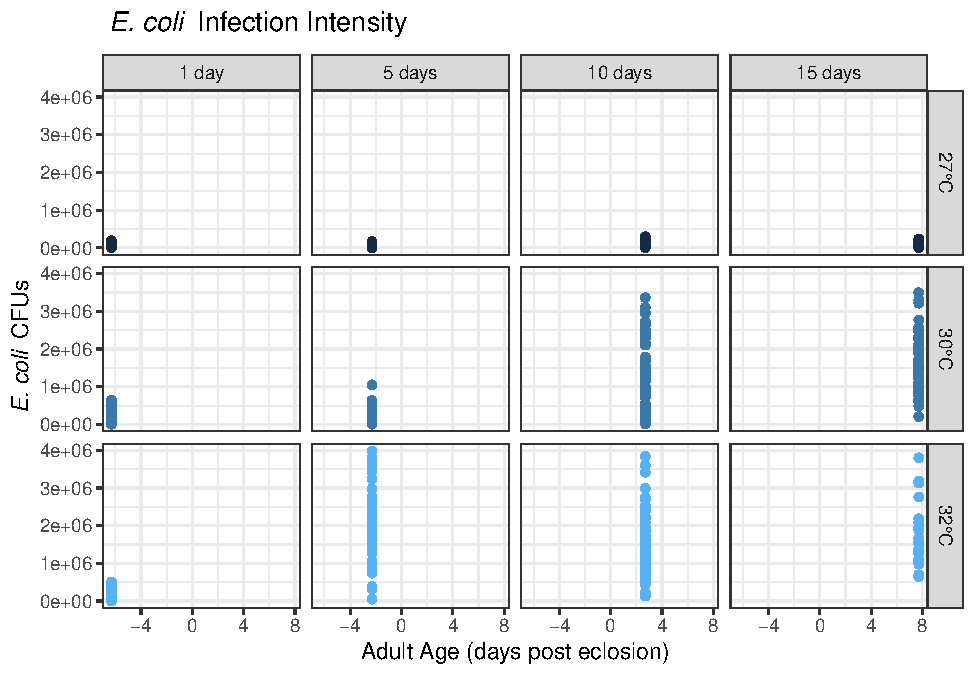
\includegraphics{Ecoli_infection_intensity_JSdata_Rmarkdownfile-081022_files/figure-latex/unnamed-chunk-1-4.pdf}

\begin{verbatim}
## Bin width defaults to 1/30 of the range of the data. Pick better value with `binwidth`.
\end{verbatim}

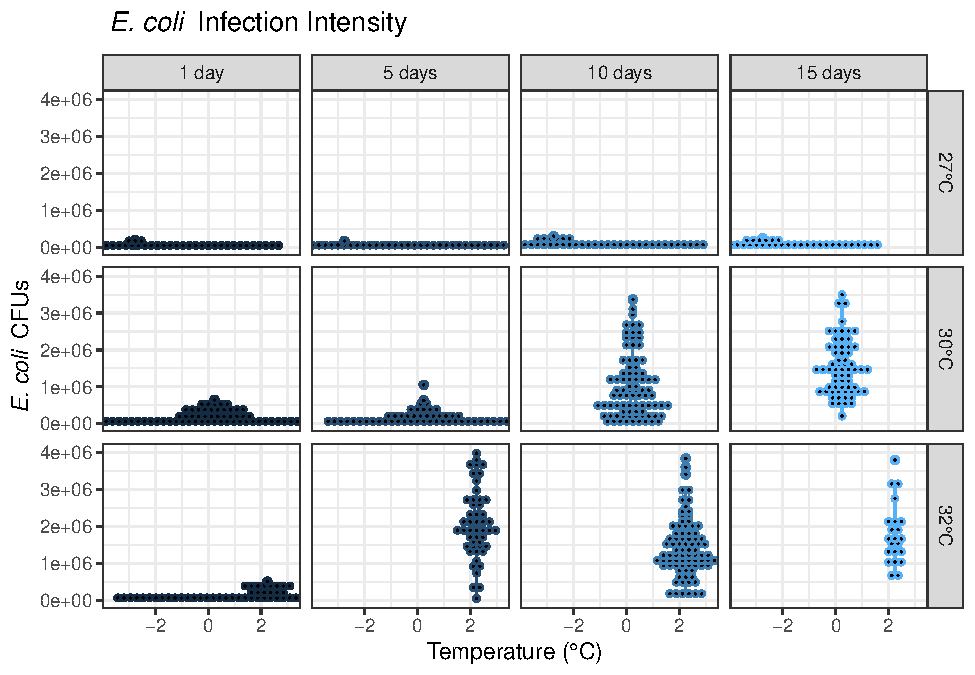
\includegraphics{Ecoli_infection_intensity_JSdata_Rmarkdownfile-081022_files/figure-latex/unnamed-chunk-1-5.pdf}

\begin{verbatim}
## Bin width defaults to 1/30 of the range of the data. Pick better value with `binwidth`.
\end{verbatim}

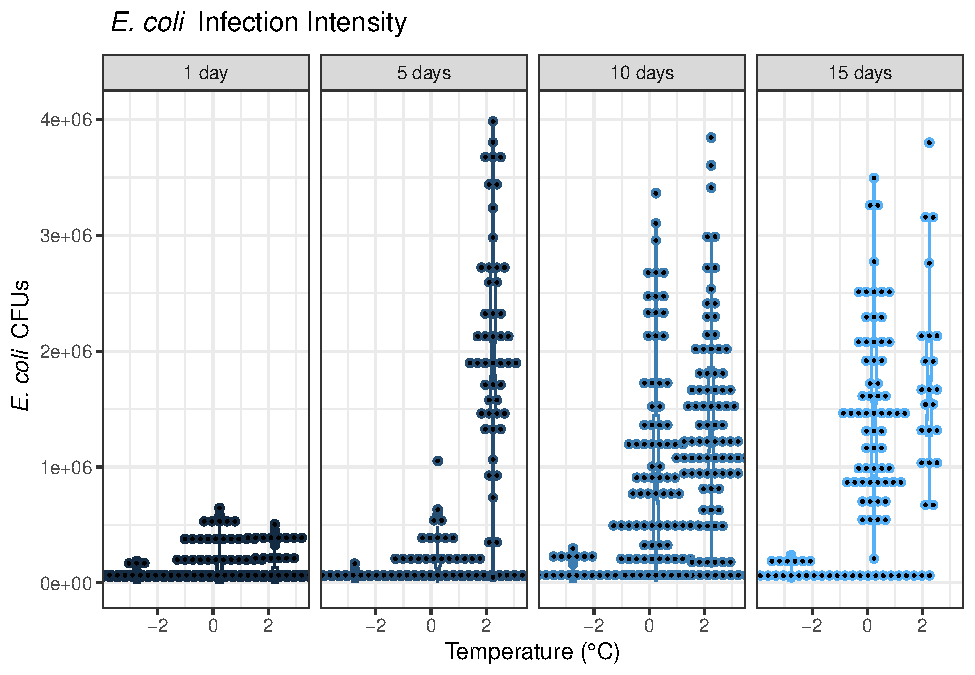
\includegraphics{Ecoli_infection_intensity_JSdata_Rmarkdownfile-081022_files/figure-latex/unnamed-chunk-1-6.pdf}

\begin{verbatim}
## Bin width defaults to 1/30 of the range of the data. Pick better value with `binwidth`.
\end{verbatim}

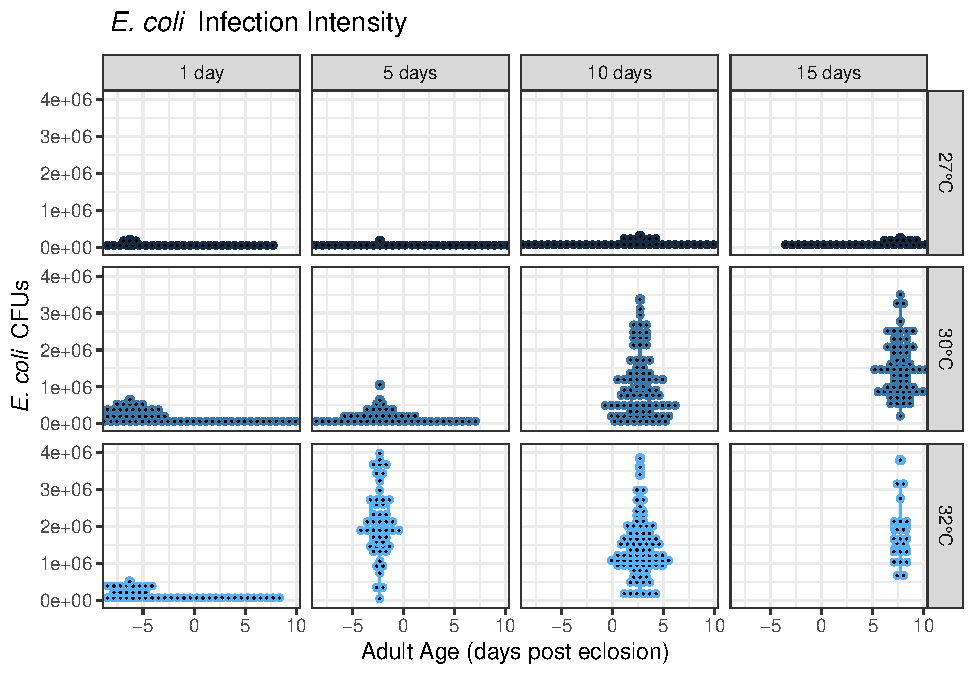
\includegraphics{Ecoli_infection_intensity_JSdata_Rmarkdownfile-081022_files/figure-latex/unnamed-chunk-1-7.pdf}
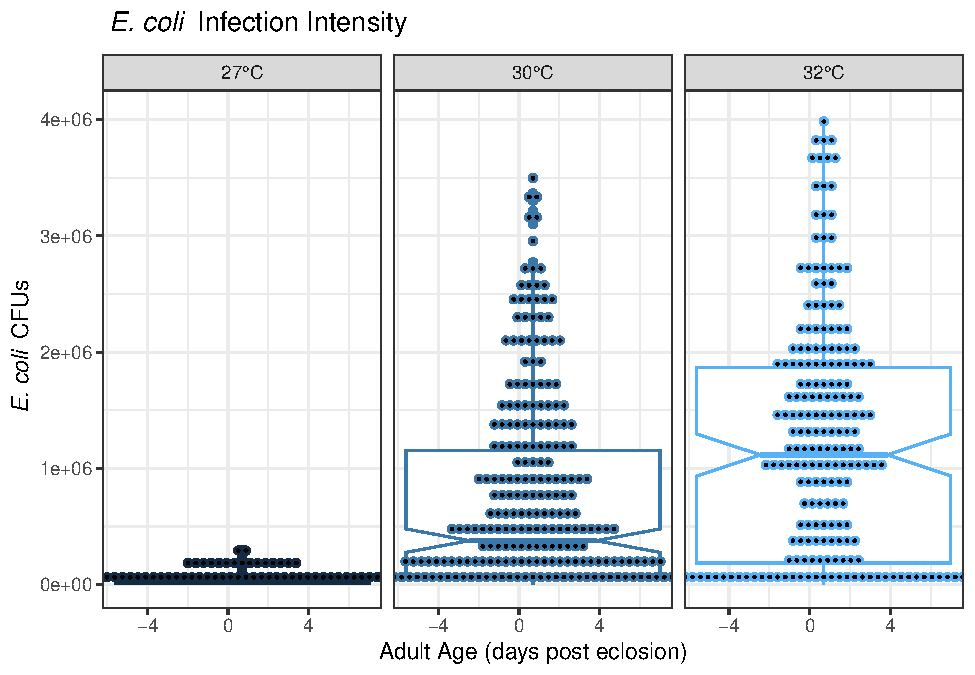
\includegraphics{Ecoli_infection_intensity_JSdata_Rmarkdownfile-081022_files/figure-latex/unnamed-chunk-1-8.pdf}

\hypertarget{data-summary-figures}{%
\subsection{Data Summary Figures}\label{data-summary-figures}}

Then, we can calculate the mean, median, SE, SD for further exploration.

\begin{Shaded}
\begin{Highlighting}[]
\CommentTok{\#calculate the mean, median, SE, sd, etc.:}
\NormalTok{II\_Summary }\OtherTok{\textless{}{-}}\NormalTok{ II\_Data }\SpecialCharTok{\%\textgreater{}\%}
  \FunctionTok{group\_by}\NormalTok{(Temperature,Age) }\SpecialCharTok{\%\textgreater{}\%}
  \FunctionTok{summarise}\NormalTok{(}\AttributeTok{mean\_CFUs =} \FunctionTok{mean}\NormalTok{(CFUs),}
            \AttributeTok{median\_CFUs =} \FunctionTok{median}\NormalTok{(CFUs),}
            \AttributeTok{sd\_CFUs =} \FunctionTok{sd}\NormalTok{(CFUs),}
            \AttributeTok{n\_CFUs =} \FunctionTok{n}\NormalTok{(),}
            \AttributeTok{SE\_CFUs =} \FunctionTok{sd}\NormalTok{(CFUs)}\SpecialCharTok{/}\FunctionTok{sqrt}\NormalTok{(}\FunctionTok{n}\NormalTok{()))}
\end{Highlighting}
\end{Shaded}

\begin{verbatim}
## `summarise()` has grouped output by 'Temperature'. You can override using the
## `.groups` argument.
\end{verbatim}

\begin{Shaded}
\begin{Highlighting}[]
\NormalTok{II\_Summary}
\end{Highlighting}
\end{Shaded}

\begin{verbatim}
## # A tibble: 12 x 7
## # Groups:   Temperature [3]
##    Temperature   Age mean_CFUs median_CFUs sd_CFUs n_CFUs SE_CFUs
##          <dbl> <dbl>     <dbl>       <dbl>   <dbl>  <int>   <dbl>
##  1          27     1    24184.        9000  40608.     49   5801.
##  2          27     5    28317.       17250  31429.     52   4358.
##  3          27    10    58540.       32000  70364.     55   9488.
##  4          27    15    60395.       43000  57644.     43   8791.
##  5          30     1   132343.       42000 174500.     83  19154.
##  6          30     5   177981.      112500 194841.     52  27020.
##  7          30    10  1032000       832000 863025.     83  94729.
##  8          30    15  1521143.     1432000 741178.     63  93380.
##  9          32     1   101000        28500 141758.     63  17860.
## 10          32     5  2066082.     1932000 940495.     49 134356.
## 11          32    10  1430341.     1254000 792195.     82  87483.
## 12          32    15  1796727.     1664000 820936.     22 175024.
\end{verbatim}

We can graph the arithmetic means with standard errors:

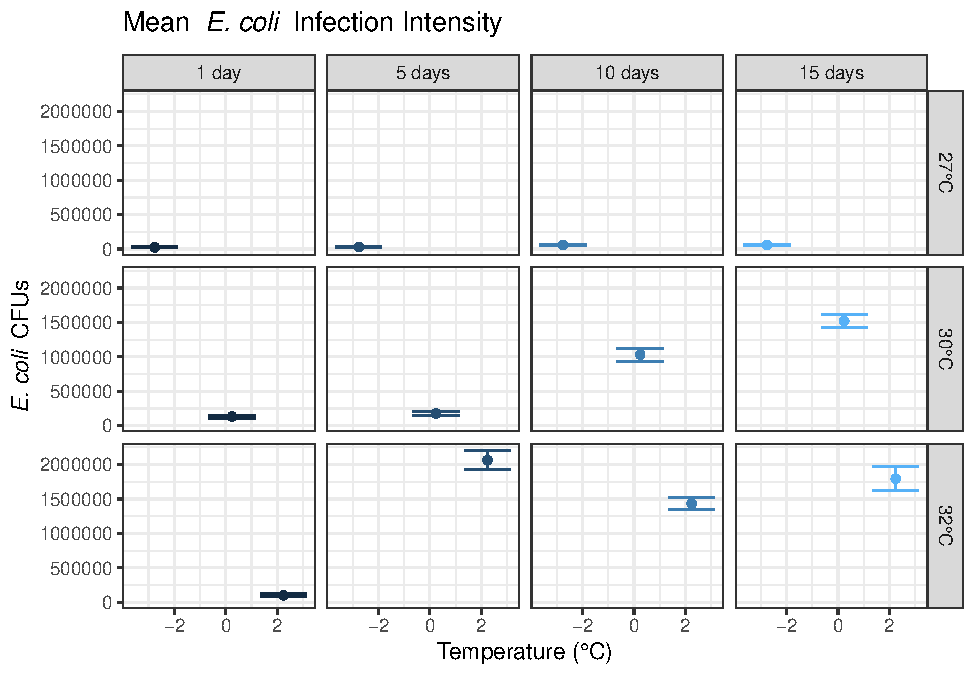
\includegraphics{Ecoli_infection_intensity_JSdata_Rmarkdownfile-081022_files/figure-latex/unnamed-chunk-3-1.pdf}

\begin{verbatim}
## # A tibble: 6 x 7
## # Groups:   Temperature [2]
##   Temperature   Age mean_CFUs median_CFUs sd_CFUs n_CFUs SE_CFUs
##         <dbl> <dbl>     <dbl>       <dbl>   <dbl>  <int>   <dbl>
## 1          27     1    24184.        9000  40608.     49   5801.
## 2          27     5    28317.       17250  31429.     52   4358.
## 3          27    10    58540.       32000  70364.     55   9488.
## 4          27    15    60395.       43000  57644.     43   8791.
## 5          30     1   132343.       42000 174500.     83  19154.
## 6          30     5   177981.      112500 194841.     52  27020.
\end{verbatim}

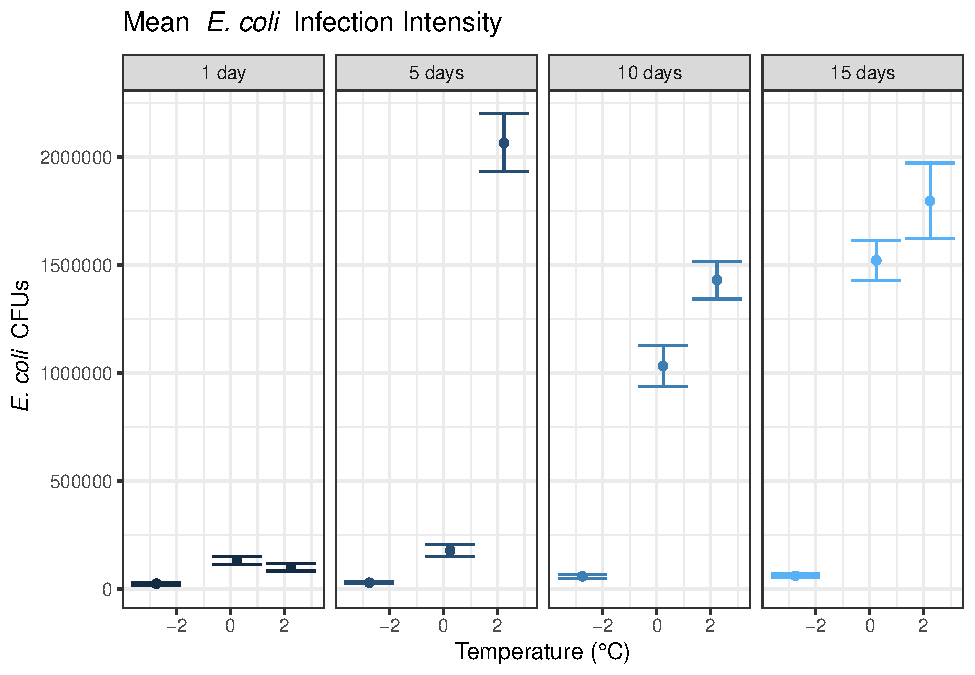
\includegraphics{Ecoli_infection_intensity_JSdata_Rmarkdownfile-081022_files/figure-latex/unnamed-chunk-3-2.pdf}
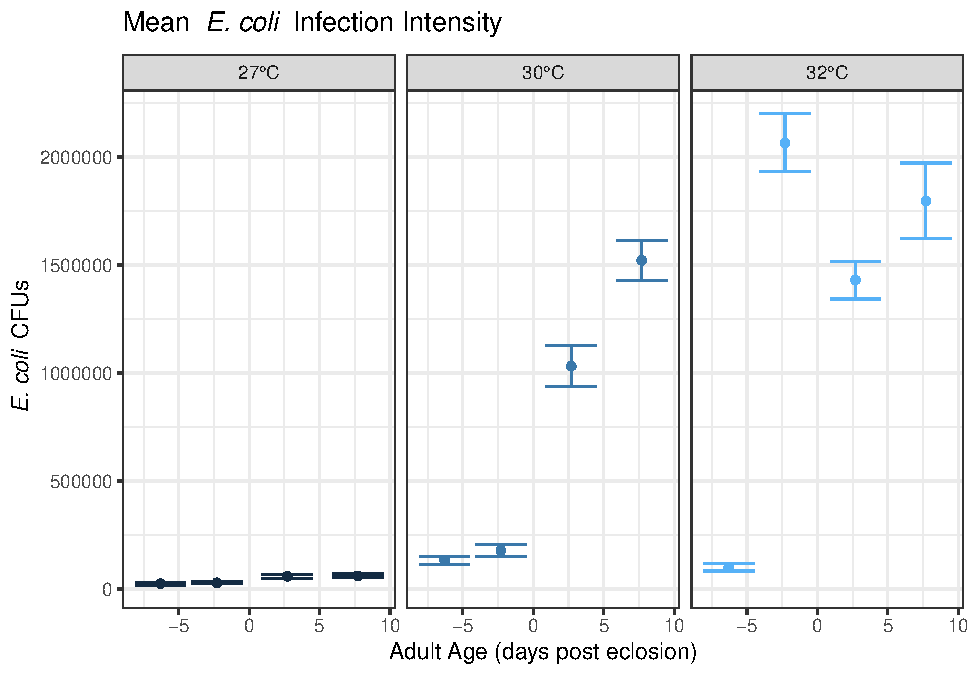
\includegraphics{Ecoli_infection_intensity_JSdata_Rmarkdownfile-081022_files/figure-latex/unnamed-chunk-3-3.pdf}

\hypertarget{preliminary-data-analysis-and-model-fitting}{%
\subsection{Preliminary Data Analysis and Model
Fitting}\label{preliminary-data-analysis-and-model-fitting}}

What is the distribution of the data? Are there any correlations? What
can we determine from assessing the variance, etc.?

We are not log-transforming the data because of the zero values at 27C,
but we don't want to exclude this data either.

Common models for count data include the negative binomial regression,
zero-inflated regression, and Poisson regression.

Helpful resources:

Delignette-Muller, M. L., \& Dutang, C. (2015). fitdistrplus: An R
Package for Fitting Distributions. Journal of Statistical Software,
64(4), 1--34. Alexander, N., 2012. Review: analysis of parasite and
other skewed counts. Tropical Medicine \& International Health 17,
684--693.. \url{doi:10.1111/j.1365-3156.2012.02987.x}
\url{https://doi.org/10.18637/jss.v064.i04}
\url{https://data.princeton.edu/wws509/r/overdispersion}
\url{https://fukamilab.github.io/BIO202/04-C-zero-data.html}
\url{https://stats.oarc.ucla.edu/r/dae/negative-binomial-regression/}
\url{https://www.jstatsoft.org/article/view/v027i08}

\begin{verbatim}
## Loading required package: GGally
\end{verbatim}

\begin{verbatim}
## Registered S3 method overwritten by 'GGally':
##   method from   
##   +.gg   ggplot2
\end{verbatim}

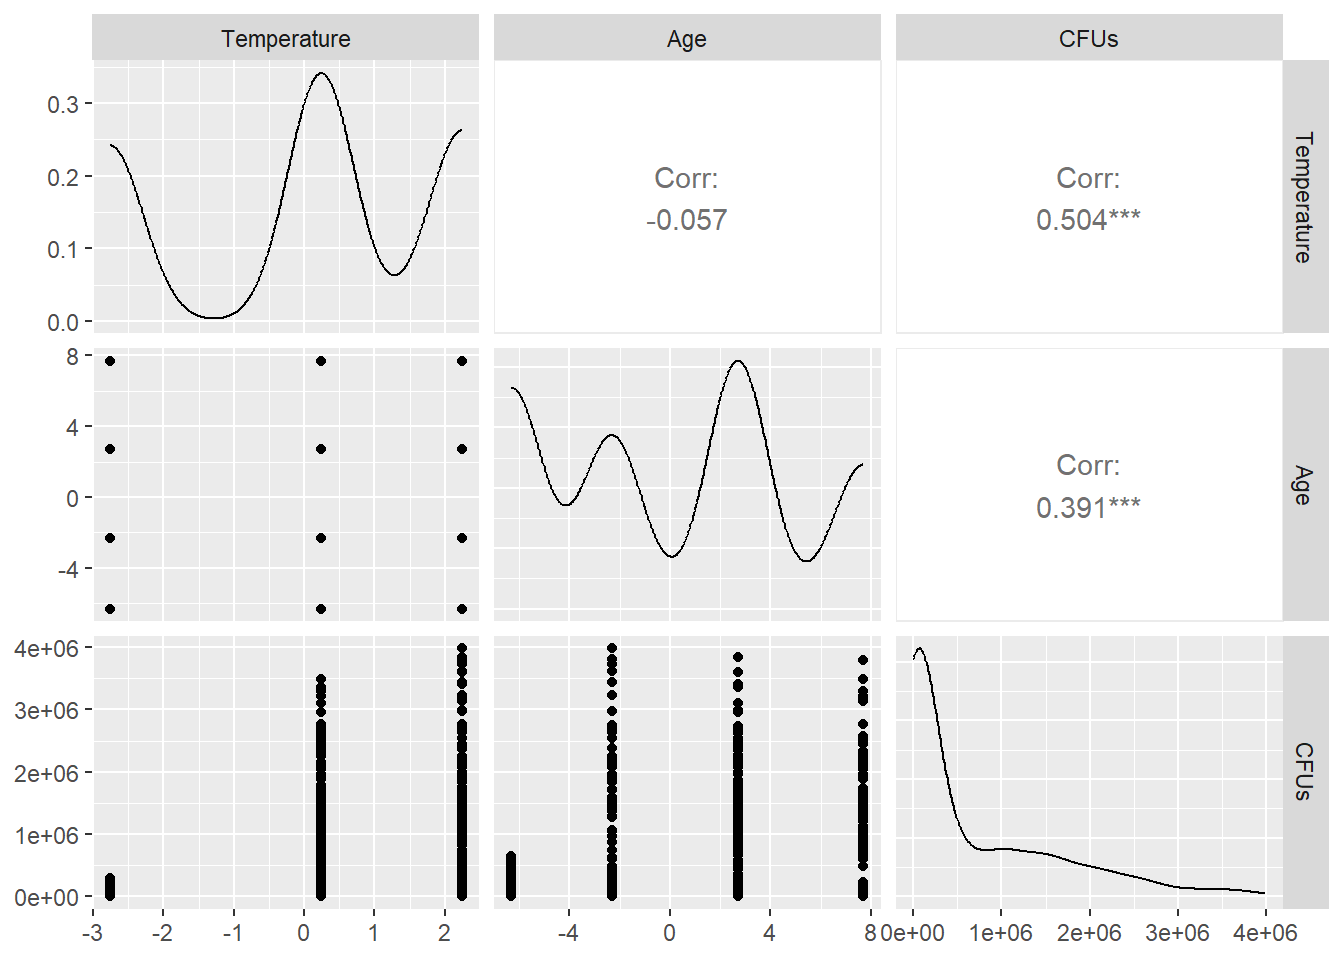
\includegraphics{Ecoli_infection_intensity_JSdata_Rmarkdownfile-081022_files/figure-latex/unnamed-chunk-4-1.pdf}
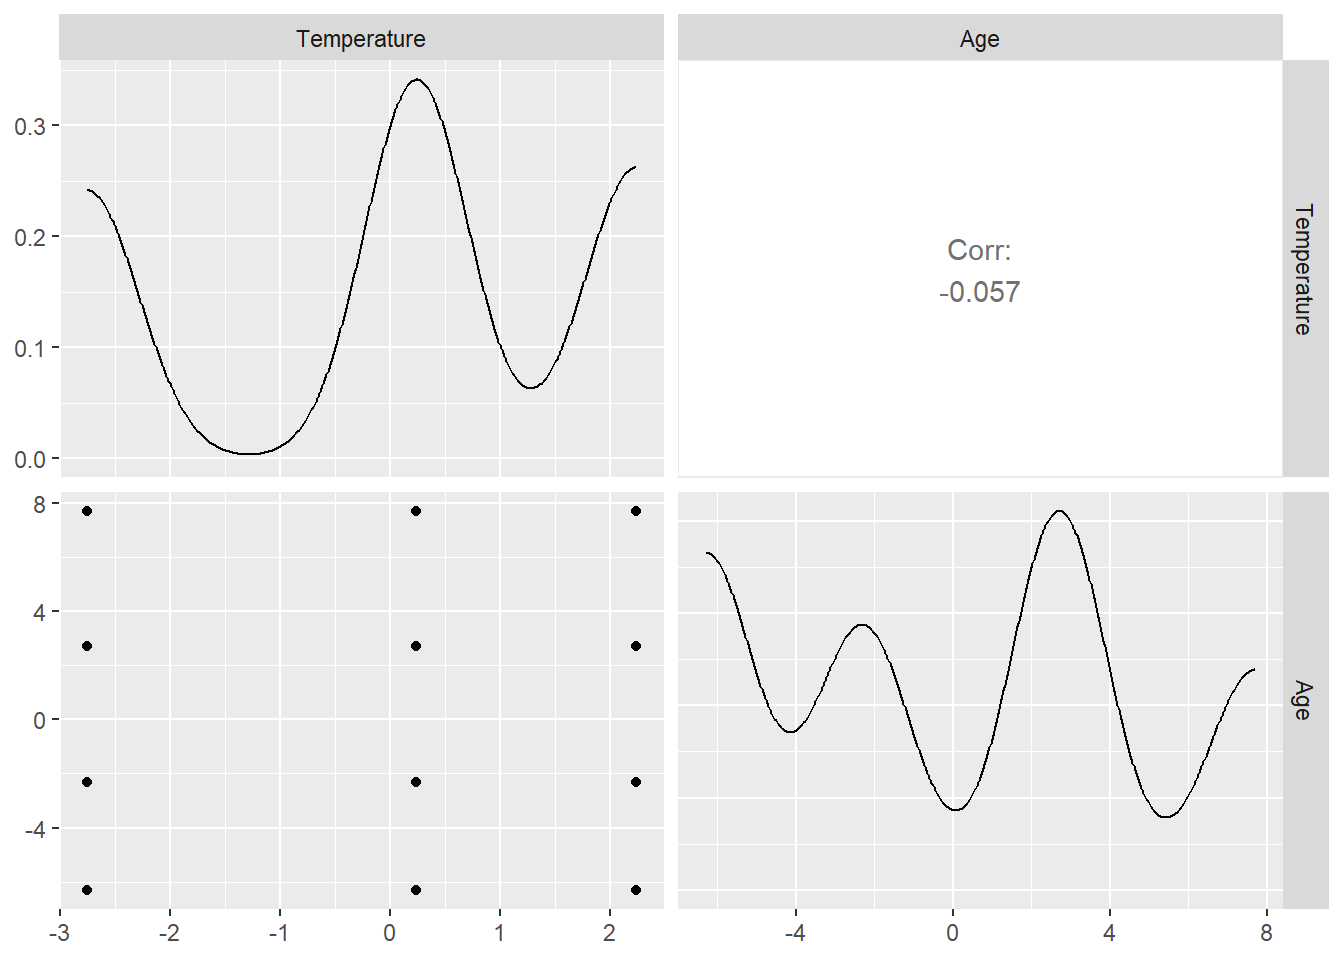
\includegraphics{Ecoli_infection_intensity_JSdata_Rmarkdownfile-081022_files/figure-latex/unnamed-chunk-4-2.pdf}

Plot histograms of the data and subsetted data.

\begin{verbatim}
## Warning in plot.window(...): "data" is not a graphical parameter
\end{verbatim}

\begin{verbatim}
## Warning in plot.xy(xy, type, ...): "data" is not a graphical parameter
\end{verbatim}

\begin{verbatim}
## Warning in axis(side = side, at = at, labels = labels, ...): "data" is not a
## graphical parameter

## Warning in axis(side = side, at = at, labels = labels, ...): "data" is not a
## graphical parameter
\end{verbatim}

\begin{verbatim}
## Warning in box(...): "data" is not a graphical parameter
\end{verbatim}

\begin{verbatim}
## Warning in title(...): "data" is not a graphical parameter
\end{verbatim}

\begin{verbatim}
## Warning in axis(...): "data" is not a graphical parameter
\end{verbatim}

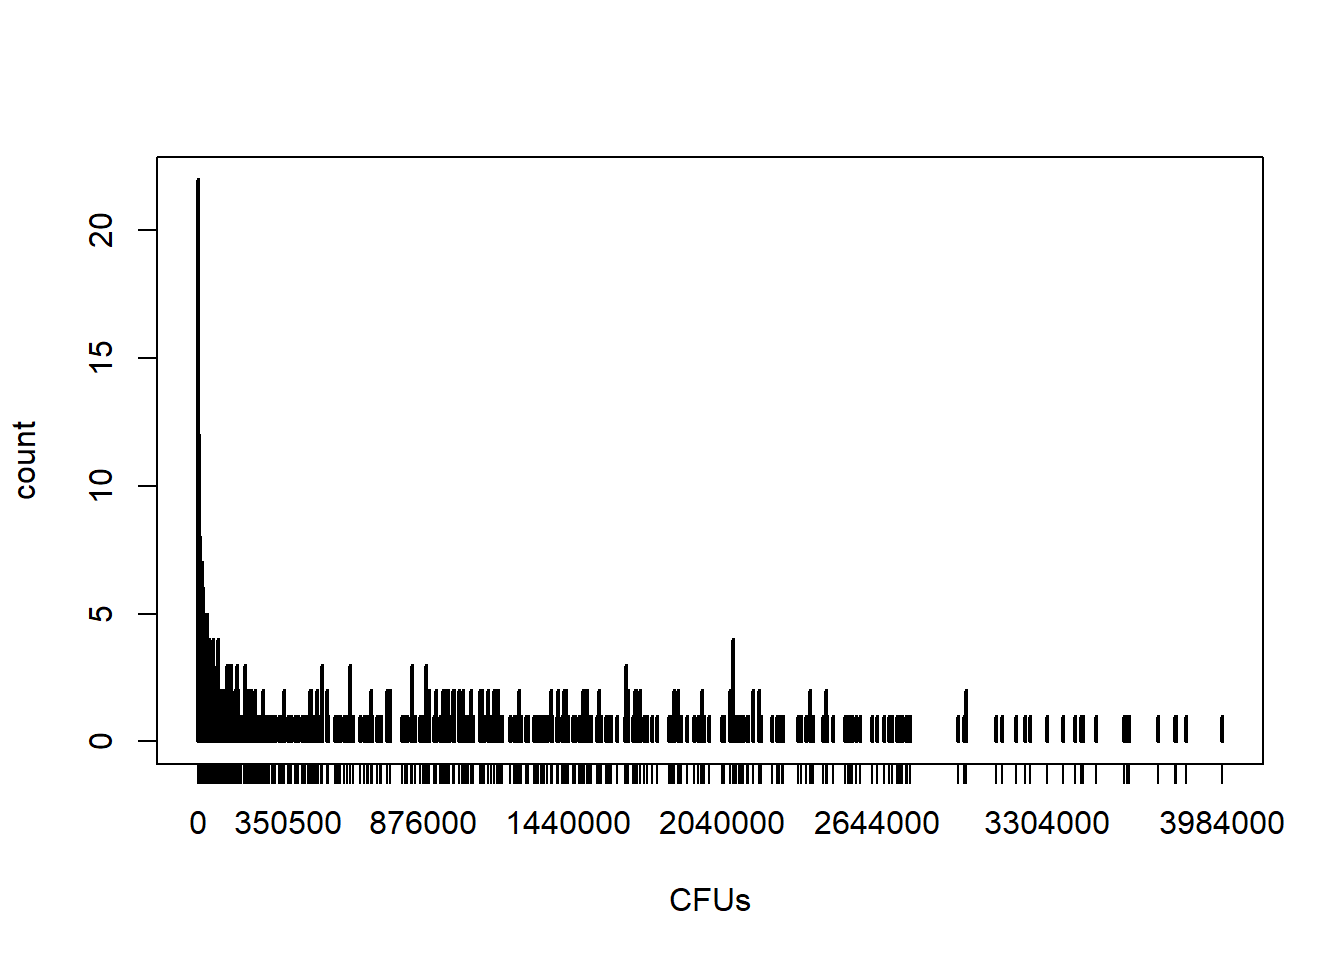
\includegraphics{Ecoli_infection_intensity_JSdata_Rmarkdownfile-081022_files/figure-latex/unnamed-chunk-5-1.pdf}
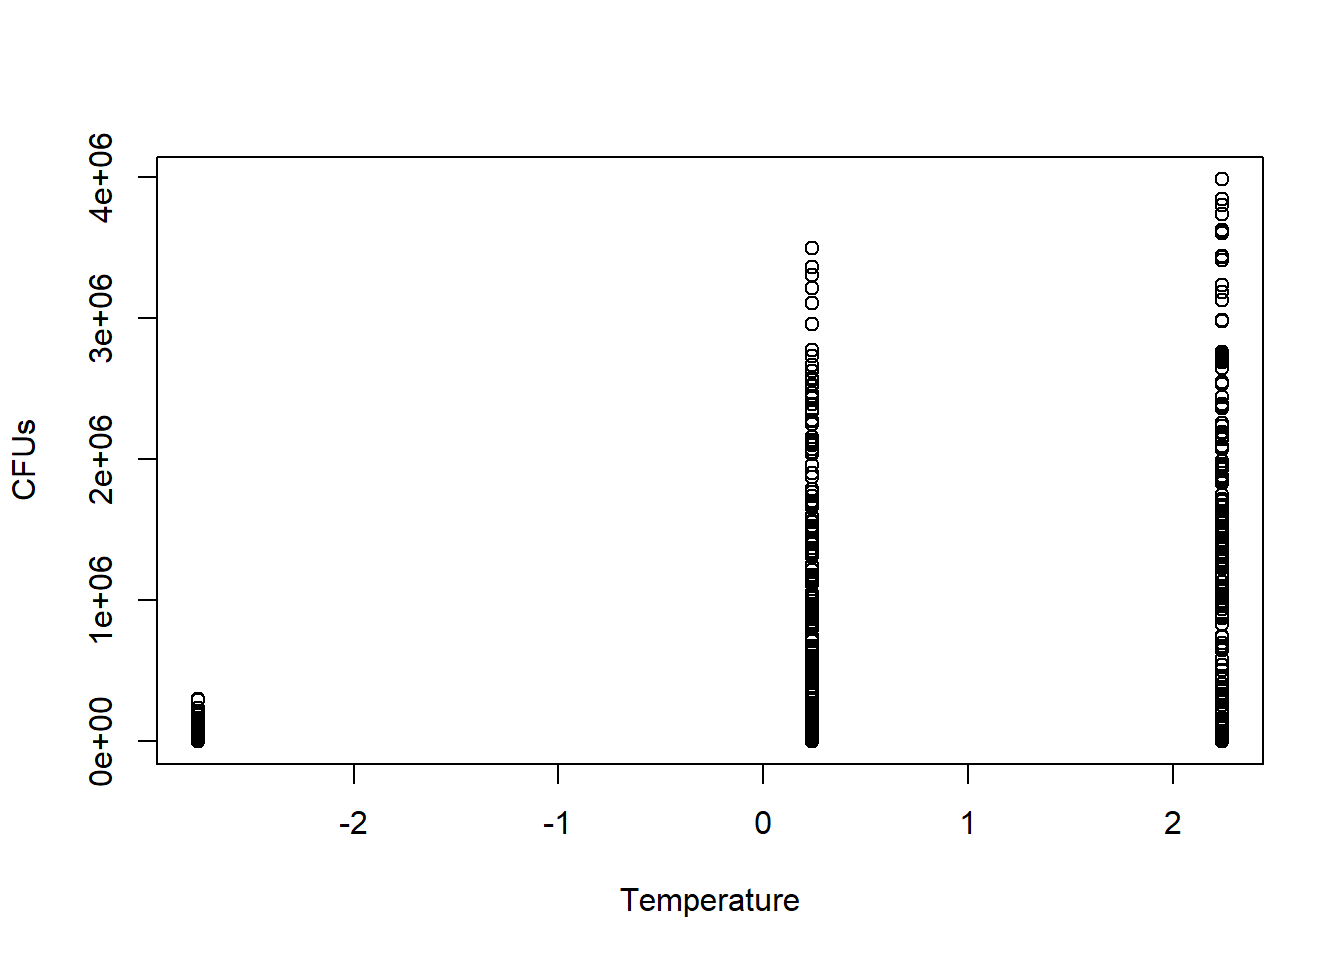
\includegraphics{Ecoli_infection_intensity_JSdata_Rmarkdownfile-081022_files/figure-latex/unnamed-chunk-5-2.pdf}
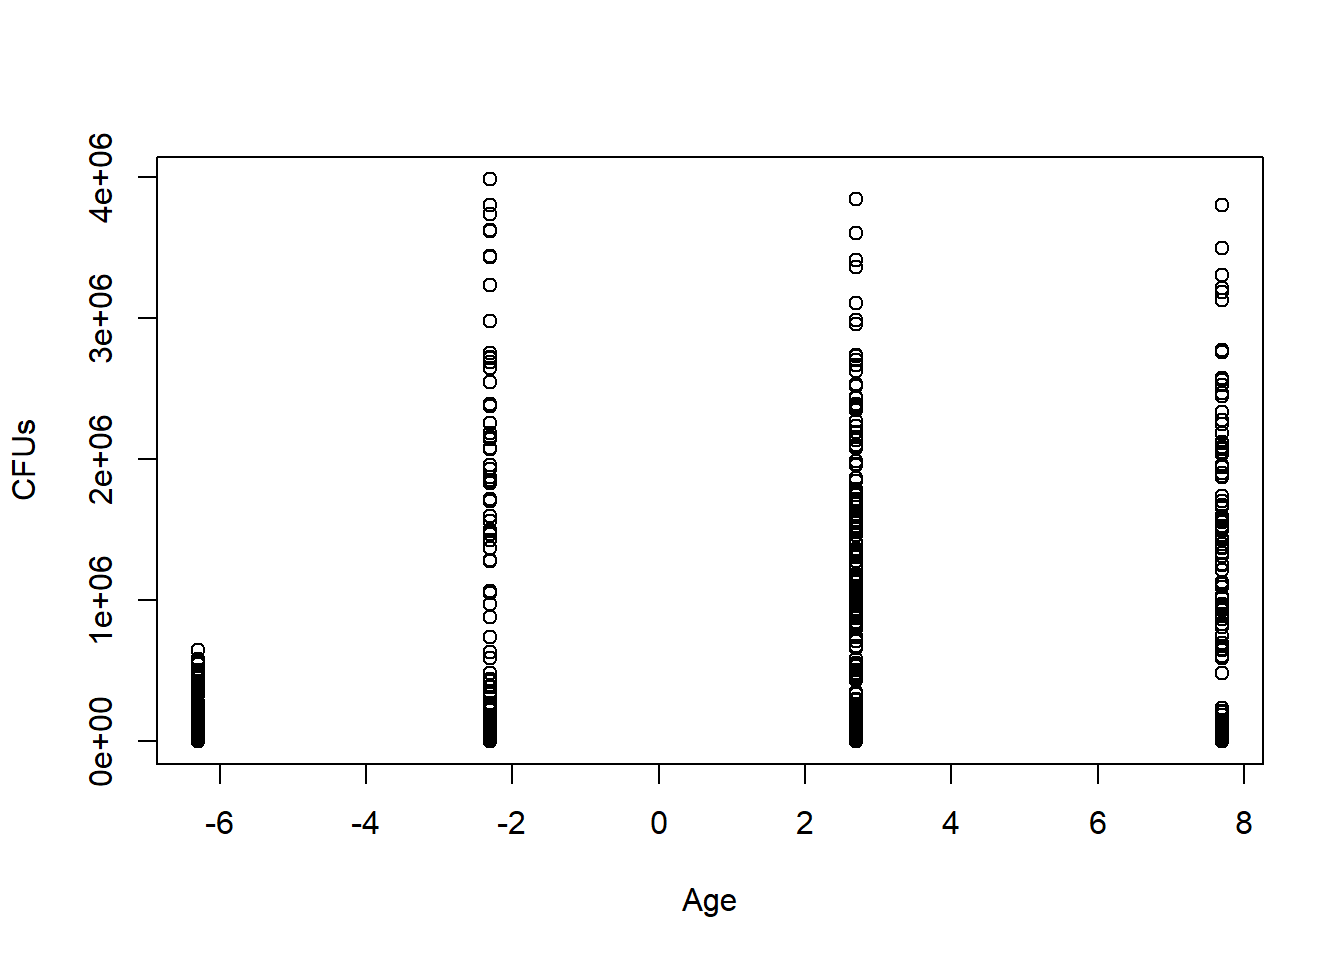
\includegraphics{Ecoli_infection_intensity_JSdata_Rmarkdownfile-081022_files/figure-latex/unnamed-chunk-5-3.pdf}
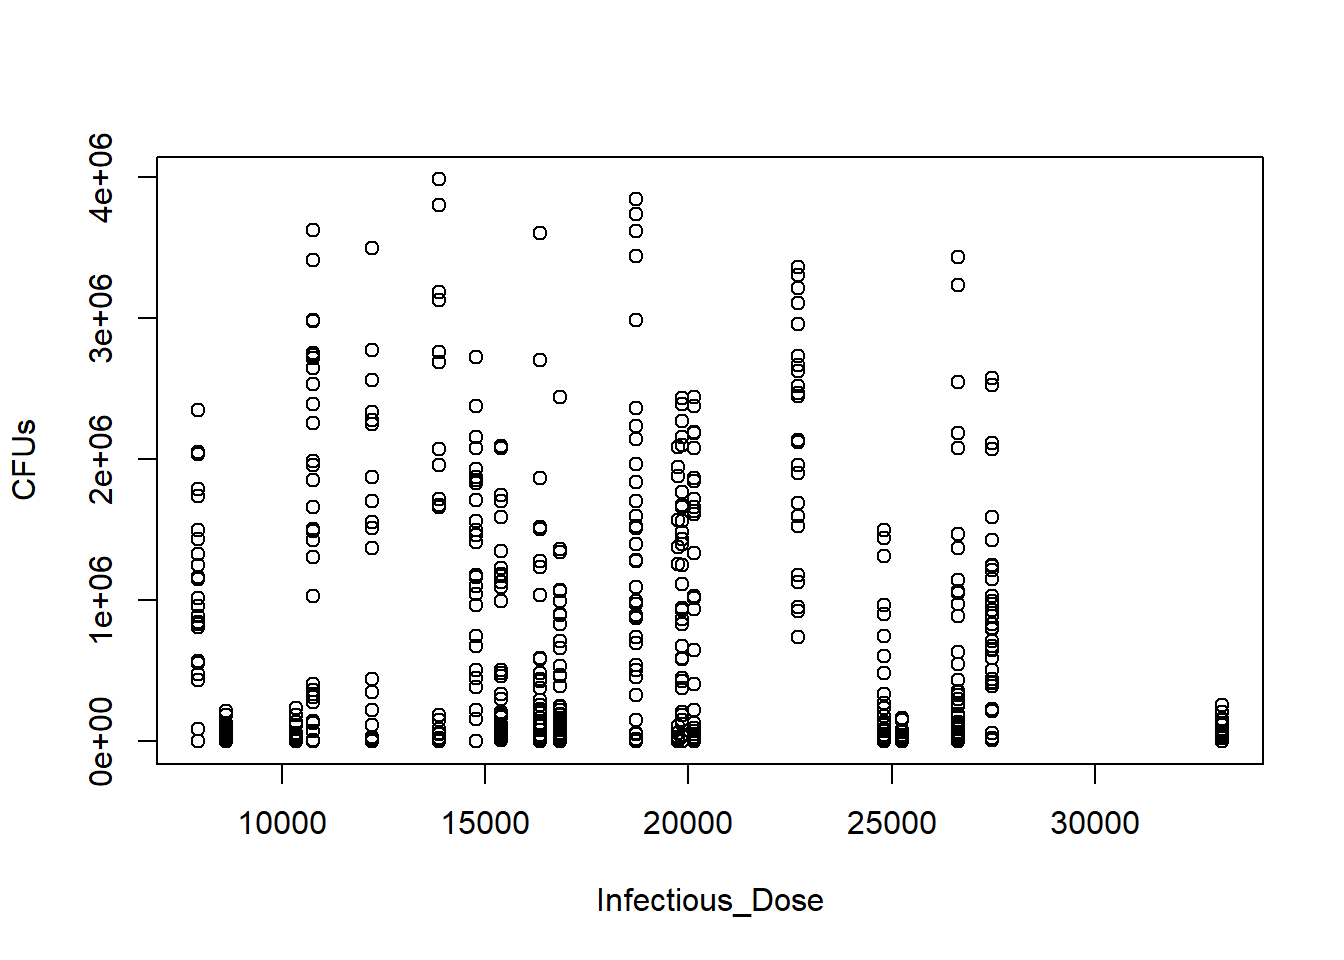
\includegraphics{Ecoli_infection_intensity_JSdata_Rmarkdownfile-081022_files/figure-latex/unnamed-chunk-5-4.pdf}
\includegraphics{Ecoli_infection_intensity_JSdata_Rmarkdownfile-081022_files/figure-latex/unnamed-chunk-5-5.pdf}
\includegraphics{Ecoli_infection_intensity_JSdata_Rmarkdownfile-081022_files/figure-latex/unnamed-chunk-5-6.pdf}
\includegraphics{Ecoli_infection_intensity_JSdata_Rmarkdownfile-081022_files/figure-latex/unnamed-chunk-5-7.pdf}

CFU data varies with Temp and Age, but not infectious dose. There also
seem to be a large number of zero count values.

\begin{Shaded}
\begin{Highlighting}[]
\CommentTok{\#what percent of the data is made up of zeros?}
\DecValTok{100}\SpecialCharTok{*}\FunctionTok{sum}\NormalTok{(II\_Data}\SpecialCharTok{$}\NormalTok{CFUs }\SpecialCharTok{==}\DecValTok{0}\NormalTok{)}\SpecialCharTok{/}\FunctionTok{nrow}\NormalTok{(II\_Data) }\CommentTok{\#3.16\%}
\end{Highlighting}
\end{Shaded}

\begin{verbatim}
## [1] 3.16092
\end{verbatim}

3.16\% of the data is made of zero-CFU counts.

What happens if we do a log(x+1) transformation to the CFU data?

\includegraphics{Ecoli_infection_intensity_JSdata_Rmarkdownfile-081022_files/figure-latex/unnamed-chunk-7-1.pdf}
\includegraphics{Ecoli_infection_intensity_JSdata_Rmarkdownfile-081022_files/figure-latex/unnamed-chunk-7-2.pdf}

Now, plot the empirical distribution and densities for the CFU and
log(x+1) transformed CFU data. Follow up with descriptive statistics of
the data -

\begin{Shaded}
\begin{Highlighting}[]
\CommentTok{\#plot the empirical distribution and density (CDF)}
\FunctionTok{plotdist}\NormalTok{(II\_Data}\SpecialCharTok{$}\NormalTok{CFUs, }\AttributeTok{histo=}\ConstantTok{TRUE}\NormalTok{,}\AttributeTok{demp=}\ConstantTok{TRUE}\NormalTok{)}
\end{Highlighting}
\end{Shaded}

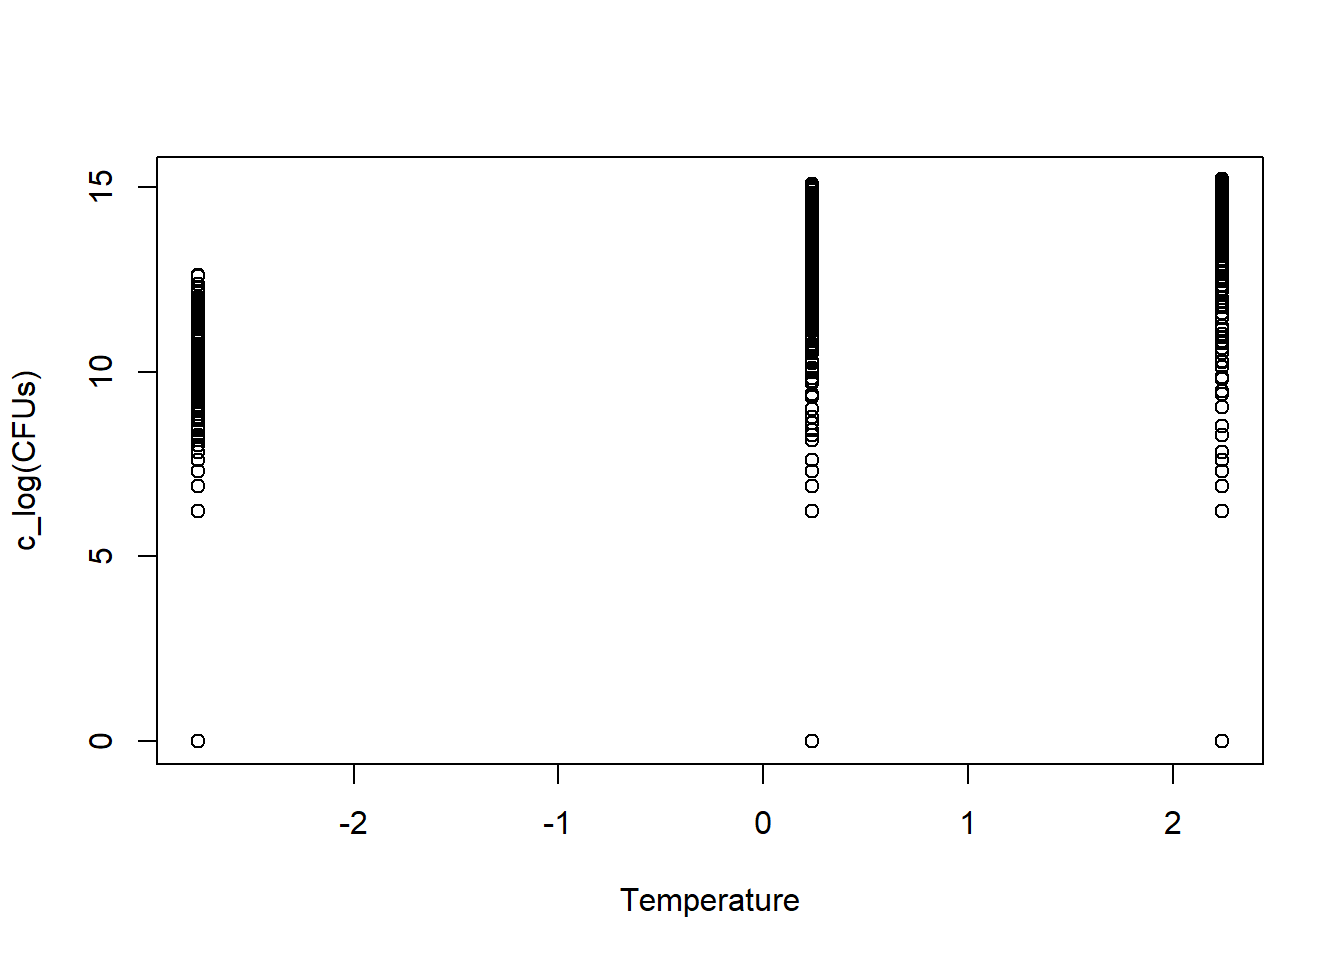
\includegraphics{Ecoli_infection_intensity_JSdata_Rmarkdownfile-081022_files/figure-latex/unnamed-chunk-8-1.pdf}

\begin{Shaded}
\begin{Highlighting}[]
\FunctionTok{plotdist}\NormalTok{(}\FunctionTok{c\_log}\NormalTok{(II\_Data}\SpecialCharTok{$}\NormalTok{CFUs),}\AttributeTok{histo=}\ConstantTok{TRUE}\NormalTok{,}\AttributeTok{demp=}\ConstantTok{TRUE}\NormalTok{)}
\end{Highlighting}
\end{Shaded}

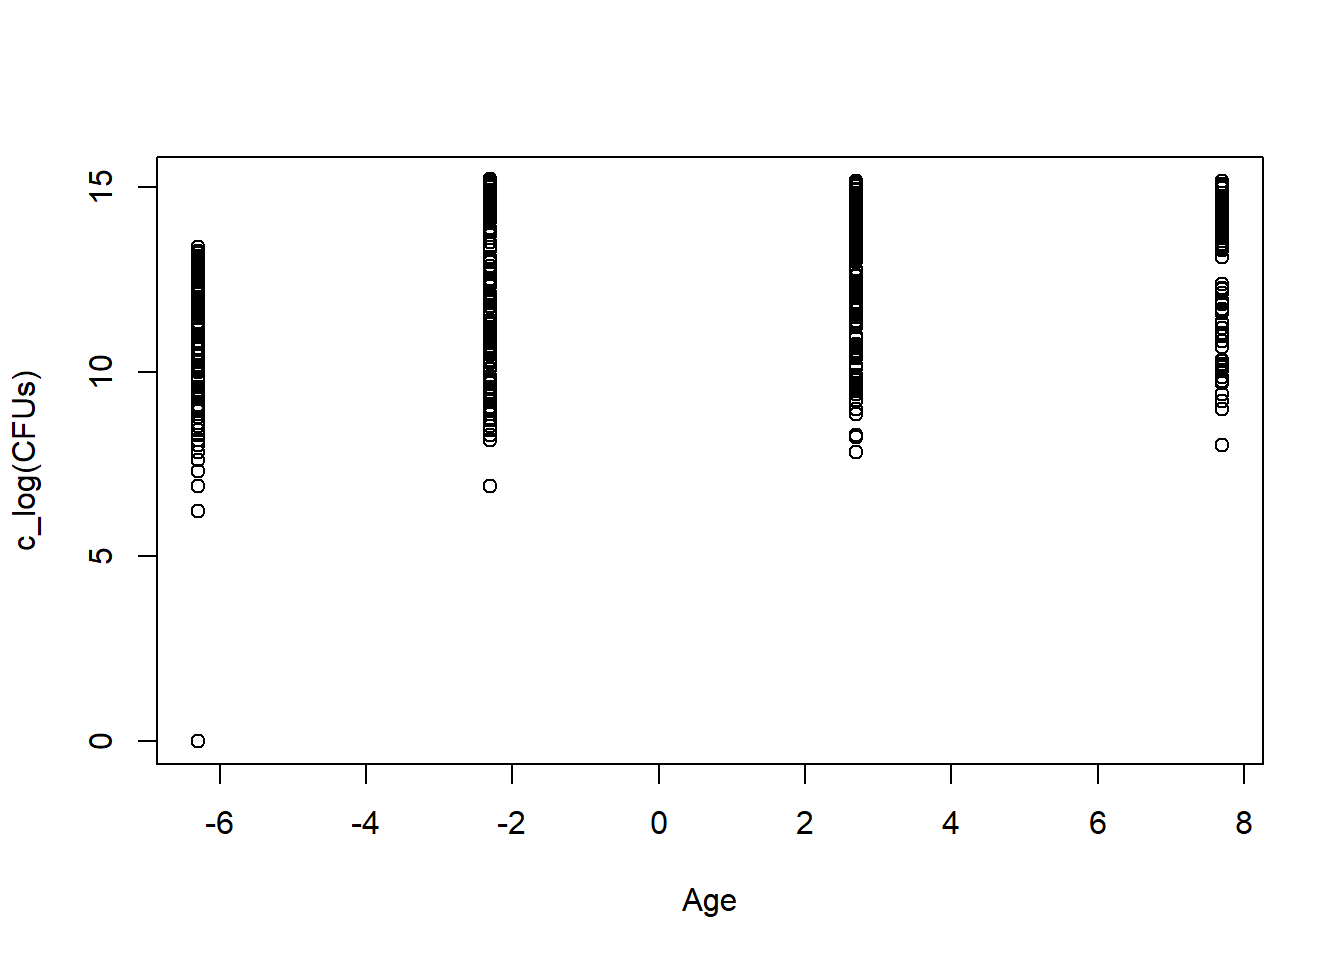
\includegraphics{Ecoli_infection_intensity_JSdata_Rmarkdownfile-081022_files/figure-latex/unnamed-chunk-8-2.pdf}

\begin{Shaded}
\begin{Highlighting}[]
\CommentTok{\#descriptive statistics of the data and graph}
\FunctionTok{descdist}\NormalTok{(II\_Data}\SpecialCharTok{$}\NormalTok{CFUs, }\AttributeTok{boot =} \DecValTok{1000}\NormalTok{)}
\end{Highlighting}
\end{Shaded}

\includegraphics{Ecoli_infection_intensity_JSdata_Rmarkdownfile-081022_files/figure-latex/unnamed-chunk-8-3.pdf}

\begin{verbatim}
## summary statistics
## ------
## min:  0   max:  3984000 
## median:  180500 
## mean:  681923.5 
## estimated sd:  906744.2 
## estimated skewness:  1.431304 
## estimated kurtosis:  4.26786
\end{verbatim}

We are estimating skewness and kurtosis, using bootstrap samples. This
is constructed by random sampling with replacement from original data
set. There is high variance regardless of bootstrapping.

How does the variance compare to the mean of the CFU data?

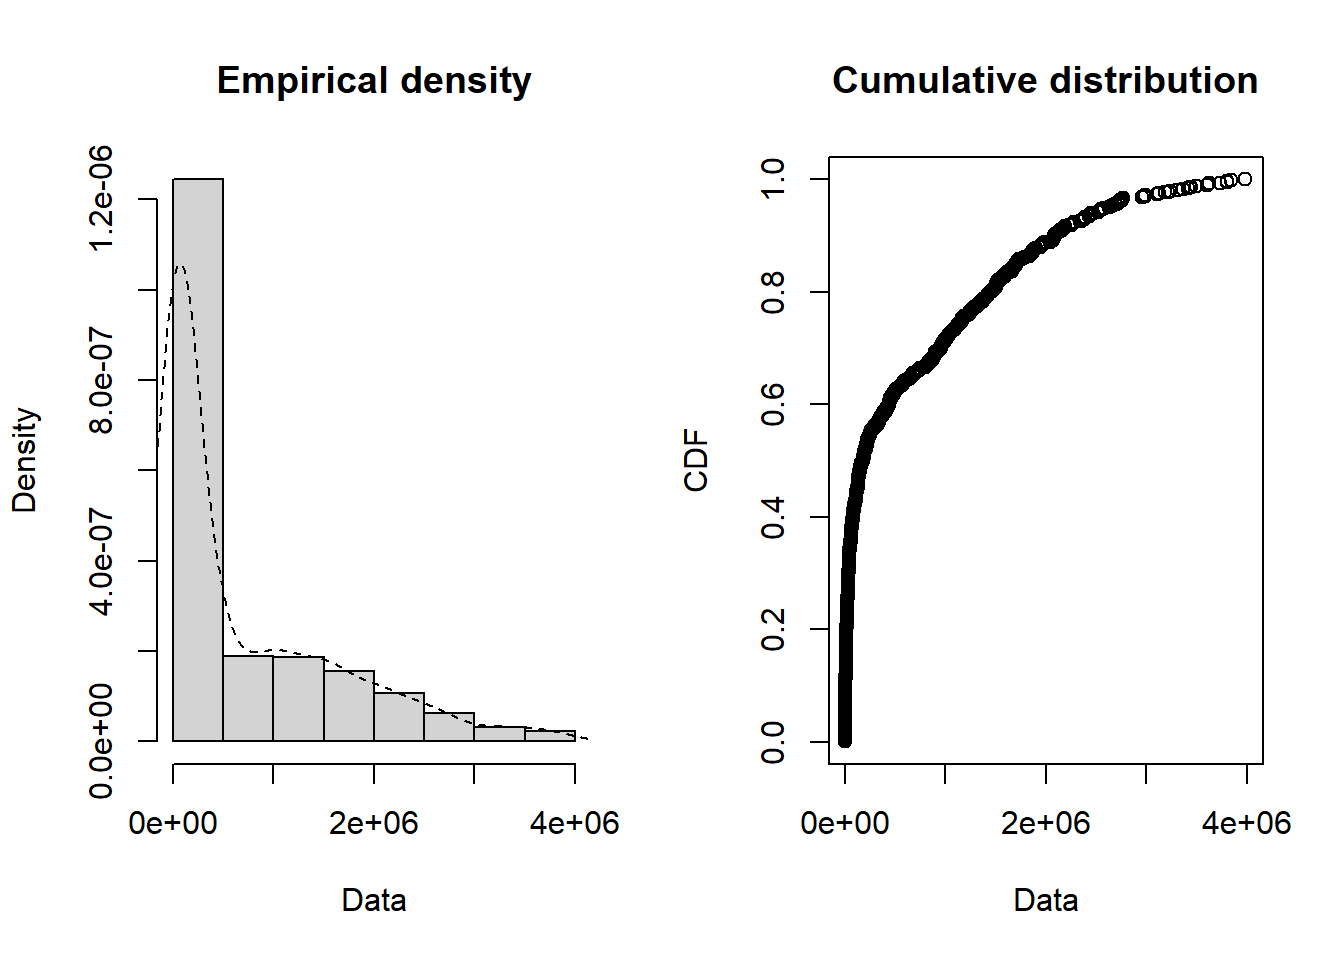
\includegraphics{Ecoli_infection_intensity_JSdata_Rmarkdownfile-081022_files/figure-latex/unnamed-chunk-9-1.pdf}

\begin{verbatim}
##         mean          var        ratio 
## 6.819235e+05 8.221851e+11 1.205685e+06
\end{verbatim}

Poisson assumption of equal mean and variance does not hold true. The
variance is greater than the mean (ratio = 1.2e6) and is considered
over-dispersed.

This suggests a Neg Binom model may be better (mean does not equal
variance, which is assumed by Poisson dist).

First, we'll look at the Poisson dist and Neg Bin dist.

\begin{Shaded}
\begin{Highlighting}[]
\CommentTok{\#assess fits:}
\CommentTok{\#check to see if the data follow a poisson distribution}
\NormalTok{fit\_poisson\_CFUs }\OtherTok{\textless{}{-}} \FunctionTok{fitdist}\NormalTok{((II\_Data}\SpecialCharTok{$}\NormalTok{CFUs),}\StringTok{"pois"}\NormalTok{)}
\FunctionTok{summary}\NormalTok{(fit\_poisson\_CFUs)}
\end{Highlighting}
\end{Shaded}

\begin{verbatim}
## Fitting of the distribution ' pois ' by maximum likelihood 
## Parameters : 
##        estimate Std. Error
## lambda 681923.5         NA
## Loglikelihood:  -381063613   AIC:  762127229   BIC:  762127233
\end{verbatim}

\begin{Shaded}
\begin{Highlighting}[]
\FunctionTok{plot}\NormalTok{(fit\_poisson\_CFUs)}
\end{Highlighting}
\end{Shaded}

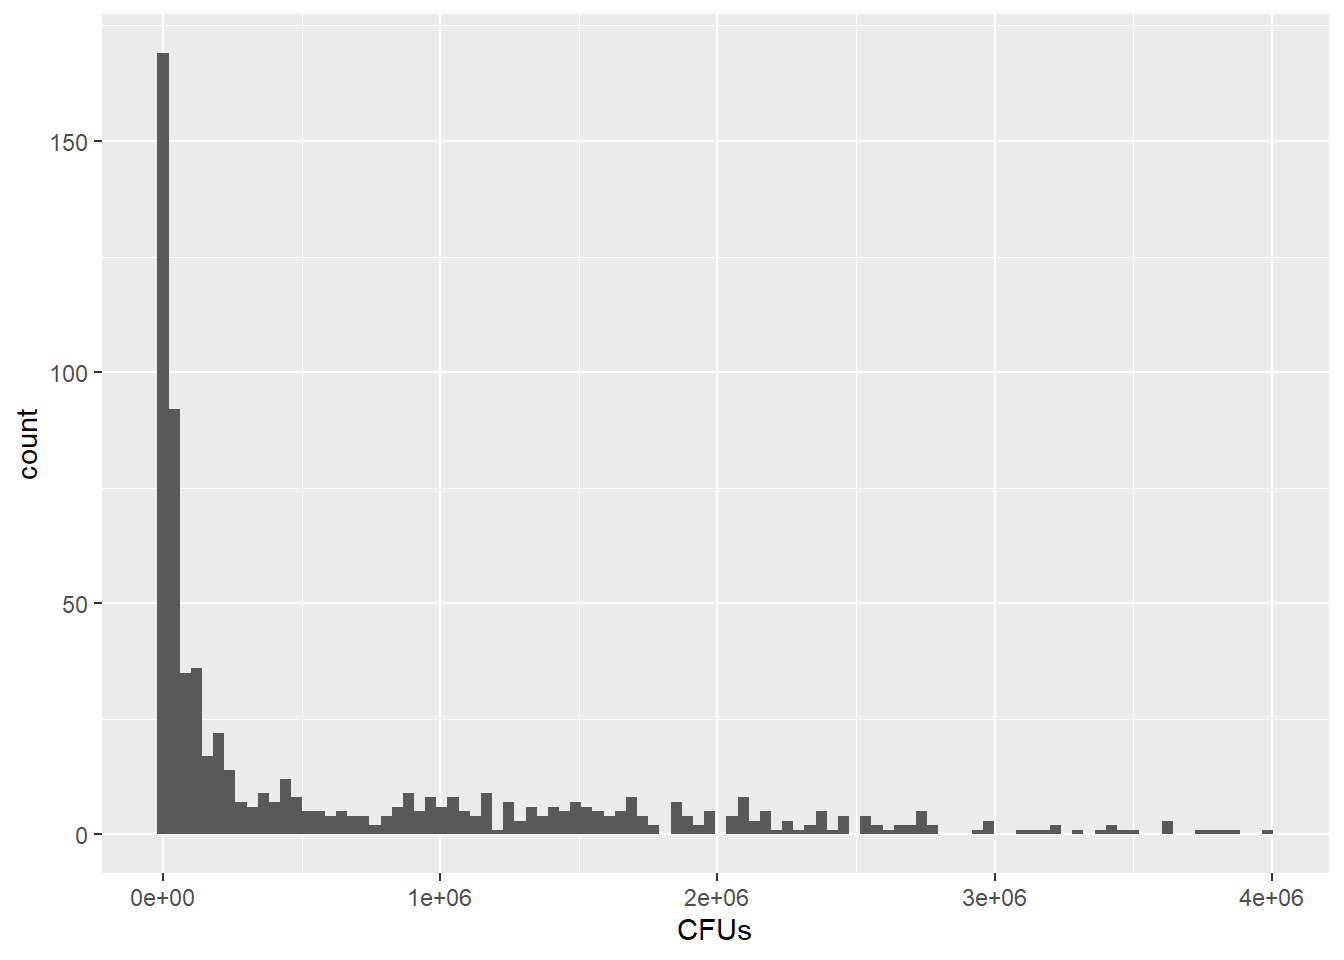
\includegraphics{Ecoli_infection_intensity_JSdata_Rmarkdownfile-081022_files/figure-latex/unnamed-chunk-10-1.pdf}

\begin{Shaded}
\begin{Highlighting}[]
\CommentTok{\#check to see if the data follow a negative binomial distribution}
\NormalTok{fit\_negbinom\_CFUs }\OtherTok{\textless{}{-}} \FunctionTok{fitdist}\NormalTok{((II\_Data}\SpecialCharTok{$}\NormalTok{CFUs), }\StringTok{"nbinom"}\NormalTok{)}
\FunctionTok{summary}\NormalTok{(fit\_negbinom\_CFUs)}
\end{Highlighting}
\end{Shaded}

\begin{verbatim}
## Fitting of the distribution ' nbinom ' by maximum likelihood 
## Parameters : 
##          estimate Std. Error
## size 3.420331e-01         NA
## mu   6.822661e+05         NA
## Loglikelihood:  -9629.12   AIC:  19262.24   BIC:  19271.33 
## Correlation matrix:
## [1] NA
\end{verbatim}

\begin{Shaded}
\begin{Highlighting}[]
\FunctionTok{plot}\NormalTok{(fit\_negbinom\_CFUs)}
\end{Highlighting}
\end{Shaded}

\includegraphics{Ecoli_infection_intensity_JSdata_Rmarkdownfile-081022_files/figure-latex/unnamed-chunk-10-2.pdf}

\begin{Shaded}
\begin{Highlighting}[]
\CommentTok{\#compare the two fits:}

\FunctionTok{par}\NormalTok{(}\AttributeTok{mfrow =} \FunctionTok{c}\NormalTok{(}\DecValTok{2}\NormalTok{, }\DecValTok{2}\NormalTok{))}
\CommentTok{\#graphics.off()}
\NormalTok{plot.legend }\OtherTok{\textless{}{-}} \FunctionTok{c}\NormalTok{(}\StringTok{"pois"}\NormalTok{, }\StringTok{"nbinom"}\NormalTok{)}
\FunctionTok{denscomp}\NormalTok{(}\FunctionTok{list}\NormalTok{(fit\_poisson\_CFUs,fit\_negbinom\_CFUs),}\AttributeTok{legendtext =}\NormalTok{ plot.legend)}
\FunctionTok{qqcomp}\NormalTok{(}\FunctionTok{list}\NormalTok{(fit\_poisson\_CFUs,fit\_negbinom\_CFUs),}\AttributeTok{legendtext =}\NormalTok{ plot.legend)}
\FunctionTok{cdfcomp}\NormalTok{(}\FunctionTok{list}\NormalTok{(fit\_poisson\_CFUs,fit\_negbinom\_CFUs),}\AttributeTok{legendtext =}\NormalTok{ plot.legend)}
\FunctionTok{ppcomp}\NormalTok{(}\FunctionTok{list}\NormalTok{(fit\_poisson\_CFUs,fit\_negbinom\_CFUs),}\AttributeTok{legendtext =}\NormalTok{ plot.legend)}
\end{Highlighting}
\end{Shaded}

\includegraphics{Ecoli_infection_intensity_JSdata_Rmarkdownfile-081022_files/figure-latex/unnamed-chunk-10-3.pdf}

\begin{Shaded}
\begin{Highlighting}[]
\CommentTok{\#check goodness of fit statistics {-} chi square for discrete data}
\FunctionTok{gofstat}\NormalTok{(}\FunctionTok{list}\NormalTok{(fit\_negbinom\_CFUs, fit\_poisson\_CFUs),}
        \AttributeTok{fitnames =} \FunctionTok{c}\NormalTok{(}\StringTok{"nbinom"}\NormalTok{, }\StringTok{"pois"}\NormalTok{))}
\end{Highlighting}
\end{Shaded}

\begin{verbatim}
## Chi-squared statistic:  109.6618 Inf 
## Degree of freedom of the Chi-squared distribution:  20 21 
## Chi-squared p-value:  2.263674e-14 0 
##    the p-value may be wrong with some theoretical counts < 5  
## Chi-squared table:
##            obscounts theo nbinom theo pois
## <= 500            30    45.79180         0
## <= 3000           30    38.66537         0
## <= 6500           29    25.51343         0
## <= 11000          29    21.60291         0
## <= 16000          33    17.89404         0
## <= 25000          32    24.44854         0
## <= 35000          30    20.96379         0
## <= 47000          29    20.34635         0
## <= 71000          29    31.86313         0
## <= 106000         29    35.05328         0
## <= 135000         29    23.21798         0
## <= 188000         29    34.37366         0
## <= 272000         29    41.78116         0
## <= 430000         29    56.26156         0
## <= 592000         31    41.36140         0
## <= 888000         31    53.08861       696
## <= 1052000        29    21.73324         0
## <= 1276000        29    23.91389         0
## <= 1504000        30    19.32710         0
## <= 1720000        30    14.84938         0
## <= 2080000        30    19.27904         0
## <= 2472000        29    15.43783         0
## > 2472000         41    49.23252         0
## 
## Goodness-of-fit criteria
##                                  nbinom      pois
## Akaike's Information Criterion 19262.24 762127229
## Bayesian Information Criterion 19271.33 762127233
\end{verbatim}

\begin{Shaded}
\begin{Highlighting}[]
\CommentTok{\#negative binomial model is a much better fit than poisson}

\CommentTok{\#for the log CFUs dist:}
\NormalTok{fit\_norm\_logCFUs }\OtherTok{\textless{}{-}} \FunctionTok{fitdist}\NormalTok{((II\_Data}\SpecialCharTok{$}\NormalTok{logCFUs),}\StringTok{"norm"}\NormalTok{)}
\FunctionTok{summary}\NormalTok{(fit\_norm\_logCFUs)}
\end{Highlighting}
\end{Shaded}

\begin{verbatim}
## Fitting of the distribution ' norm ' by maximum likelihood 
## Parameters : 
##       estimate Std. Error
## mean 11.555800 0.11575962
## sd    3.053948 0.08185437
## Loglikelihood:  -1764.62   AIC:  3533.24   BIC:  3542.331 
## Correlation matrix:
##               mean            sd
## mean  1.000000e+00 -2.693079e-10
## sd   -2.693079e-10  1.000000e+00
\end{verbatim}

\begin{Shaded}
\begin{Highlighting}[]
\FunctionTok{plot}\NormalTok{(fit\_norm\_logCFUs)}
\end{Highlighting}
\end{Shaded}

\includegraphics{Ecoli_infection_intensity_JSdata_Rmarkdownfile-081022_files/figure-latex/unnamed-chunk-10-4.pdf}

\begin{Shaded}
\begin{Highlighting}[]
\CommentTok{\#fit\_poisson\_logCFUs \textless{}{-} fitdist((II\_Data$logCFUs),"pois")}

\NormalTok{fit\_exp\_logCFUs }\OtherTok{\textless{}{-}} \FunctionTok{fitdist}\NormalTok{((II\_Data}\SpecialCharTok{$}\NormalTok{logCFUs),}\StringTok{"exp"}\NormalTok{)}
\FunctionTok{plot}\NormalTok{(fit\_exp\_logCFUs) }\CommentTok{\#not good}
\end{Highlighting}
\end{Shaded}

\includegraphics{Ecoli_infection_intensity_JSdata_Rmarkdownfile-081022_files/figure-latex/unnamed-chunk-10-5.pdf}

\begin{Shaded}
\begin{Highlighting}[]
\DocumentationTok{\#\#\#\#\#\#\#\#\#\#\#\#\#\#}
\DocumentationTok{\#\#model fitting: }
\CommentTok{\#fit Poisson, quasiPoisson, and negative binomial distributions with log link (modeling the mean not the actual data using log link)}
\NormalTok{glmPoisson }\OtherTok{\textless{}{-}} \FunctionTok{glm}\NormalTok{(CFUs }\SpecialCharTok{\textasciitilde{}}\NormalTok{ Temperature}\SpecialCharTok{*}\NormalTok{Age, }\AttributeTok{data=}\NormalTok{II\_Data, }\AttributeTok{family =} \FunctionTok{poisson}\NormalTok{(}\AttributeTok{link =} \StringTok{"log"}\NormalTok{))}
\NormalTok{glmQuasiPoisson }\OtherTok{\textless{}{-}} \FunctionTok{glm}\NormalTok{(CFUs }\SpecialCharTok{\textasciitilde{}}\NormalTok{ Temperature}\SpecialCharTok{*}\NormalTok{Age, }\AttributeTok{data=}\NormalTok{II\_Data, }\AttributeTok{family =} \FunctionTok{quasipoisson}\NormalTok{(}\AttributeTok{link =} \StringTok{"log"}\NormalTok{))}
\NormalTok{glmNegBinomial }\OtherTok{\textless{}{-}} \FunctionTok{glm.nb}\NormalTok{(CFUs }\SpecialCharTok{\textasciitilde{}}\NormalTok{ Temperature}\SpecialCharTok{*}\NormalTok{Age, }\AttributeTok{data=}\NormalTok{II\_Data,}\AttributeTok{link=}\StringTok{"log"}\NormalTok{)}
\NormalTok{glmNegBinomial\_additive }\OtherTok{\textless{}{-}} \FunctionTok{glm.nb}\NormalTok{(CFUs }\SpecialCharTok{\textasciitilde{}}\NormalTok{ Temperature}\SpecialCharTok{+}\NormalTok{Age, }\AttributeTok{data=}\NormalTok{II\_Data,}\AttributeTok{link=}\StringTok{"log"}\NormalTok{) }\CommentTok{\#leaves out interaction term}
\end{Highlighting}
\end{Shaded}

\begin{Shaded}
\begin{Highlighting}[]
\CommentTok{\#check models:}
\FunctionTok{summary}\NormalTok{(glmPoisson) }
\end{Highlighting}
\end{Shaded}

\begin{verbatim}
## 
## Call:
## glm(formula = CFUs ~ Temperature * Age, family = poisson(link = "log"), 
##     data = II_Data)
## 
## Deviance Residuals: 
##     Min       1Q   Median       3Q      Max  
## -1605.5   -571.9   -232.1    173.0   2449.6  
## 
## Coefficients:
##                   Estimate Std. Error z value Pr(>|z|)    
## (Intercept)     -8.669e+00  2.924e-03   -2965   <2e-16 ***
## Temperature      6.850e-01  9.335e-05    7338   <2e-16 ***
## Age              6.653e-01  2.449e-04    2716   <2e-16 ***
## Temperature:Age -1.739e-02  7.866e-06   -2211   <2e-16 ***
## ---
## Signif. codes:  0 '***' 0.001 '**' 0.01 '*' 0.05 '.' 0.1 ' ' 1
## 
## (Dispersion parameter for poisson family taken to be 1)
## 
##     Null deviance: 762117945  on 695  degrees of freedom
## Residual deviance: 342540627  on 692  degrees of freedom
## AIC: 342549916
## 
## Number of Fisher Scoring iterations: 6
\end{verbatim}

\begin{Shaded}
\begin{Highlighting}[]
\CommentTok{\#Residual deviance: 342540627  on 692  degrees of freedom}
\CommentTok{\#AIC: 342549916}

\FunctionTok{summary}\NormalTok{(glmQuasiPoisson)}
\end{Highlighting}
\end{Shaded}

\begin{verbatim}
## 
## Call:
## glm(formula = CFUs ~ Temperature * Age, family = quasipoisson(link = "log"), 
##     data = II_Data)
## 
## Deviance Residuals: 
##     Min       1Q   Median       3Q      Max  
## -1605.5   -571.9   -232.1    173.0   2449.6  
## 
## Coefficients:
##                  Estimate Std. Error t value Pr(>|t|)    
## (Intercept)     -8.669337   2.169038  -3.997 7.11e-05 ***
## Temperature      0.685033   0.069243   9.893  < 2e-16 ***
## Age              0.665303   0.181666   3.662 0.000269 ***
## Temperature:Age -0.017391   0.005835  -2.981 0.002978 ** 
## ---
## Signif. codes:  0 '***' 0.001 '**' 0.01 '*' 0.05 '.' 0.1 ' ' 1
## 
## (Dispersion parameter for quasipoisson family taken to be 550206.2)
## 
##     Null deviance: 762117945  on 695  degrees of freedom
## Residual deviance: 342540627  on 692  degrees of freedom
## AIC: NA
## 
## Number of Fisher Scoring iterations: 6
\end{verbatim}

\begin{Shaded}
\begin{Highlighting}[]
\CommentTok{\#Residual deviance: 342540627  on 692  degrees of freedom}
\CommentTok{\#AIC: NA}

\FunctionTok{summary}\NormalTok{(glmNegBinomial)}
\end{Highlighting}
\end{Shaded}

\begin{verbatim}
## 
## Call:
## glm.nb(formula = CFUs ~ Temperature * Age, data = II_Data, link = "log", 
##     init.theta = 0.5548731255)
## 
## Deviance Residuals: 
##     Min       1Q   Median       3Q      Max  
## -3.8496  -0.9400  -0.3797   0.2275   2.2592  
## 
## Coefficients:
##                  Estimate Std. Error z value Pr(>|z|)    
## (Intercept)     -3.559337   1.394446  -2.553   0.0107 *  
## Temperature      0.502902   0.046715  10.765  < 2e-16 ***
## Age             -0.653006   0.159179  -4.102 4.09e-05 ***
## Temperature:Age  0.027626   0.005358   5.156 2.52e-07 ***
## ---
## Signif. codes:  0 '***' 0.001 '**' 0.01 '*' 0.05 '.' 0.1 ' ' 1
## 
## (Dispersion parameter for Negative Binomial(0.5549) family taken to be 1)
## 
##     Null deviance: 1488.50  on 695  degrees of freedom
## Residual deviance:  867.08  on 692  degrees of freedom
## AIC: 18787
## 
## Number of Fisher Scoring iterations: 1
## 
## 
##               Theta:  0.5549 
##           Std. Err.:  0.0255 
## 
##  2 x log-likelihood:  -18776.9520
\end{verbatim}

\begin{Shaded}
\begin{Highlighting}[]
\FunctionTok{plot}\NormalTok{(glmNegBinomial)}
\end{Highlighting}
\end{Shaded}

\includegraphics{Ecoli_infection_intensity_JSdata_Rmarkdownfile-081022_files/figure-latex/unnamed-chunk-11-1.pdf}
\includegraphics{Ecoli_infection_intensity_JSdata_Rmarkdownfile-081022_files/figure-latex/unnamed-chunk-11-2.pdf}
\includegraphics{Ecoli_infection_intensity_JSdata_Rmarkdownfile-081022_files/figure-latex/unnamed-chunk-11-3.pdf}
\includegraphics{Ecoli_infection_intensity_JSdata_Rmarkdownfile-081022_files/figure-latex/unnamed-chunk-11-4.pdf}

\begin{Shaded}
\begin{Highlighting}[]
\CommentTok{\#Residual deviance:  867.08  on 692  degrees of freedom}
\CommentTok{\#AIC: 18787}
\CommentTok{\# 2 x log{-}likelihood:  {-}18776.9520  }
\CommentTok{\#Theta:  0.5549 }
\CommentTok{\#Std. Err.:  0.0255}


\FunctionTok{summary}\NormalTok{(glmNegBinomial\_additive)}
\end{Highlighting}
\end{Shaded}

\begin{verbatim}
## 
## Call:
## glm.nb(formula = CFUs ~ Temperature + Age, data = II_Data, link = "log", 
##     init.theta = 0.5454901466)
## 
## Deviance Residuals: 
##     Min       1Q   Median       3Q      Max  
## -3.8757  -0.9157  -0.3703   0.2401   2.8469  
## 
## Coefficients:
##             Estimate Std. Error z value Pr(>|z|)    
## (Intercept) -8.74784    0.79860  -10.95   <2e-16 ***
## Temperature  0.67969    0.02652   25.63   <2e-16 ***
## Age          0.15995    0.01018   15.71   <2e-16 ***
## ---
## Signif. codes:  0 '***' 0.001 '**' 0.01 '*' 0.05 '.' 0.1 ' ' 1
## 
## (Dispersion parameter for Negative Binomial(0.5455) family taken to be 1)
## 
##     Null deviance: 1463.74  on 695  degrees of freedom
## Residual deviance:  868.84  on 693  degrees of freedom
## AIC: 18801
## 
## Number of Fisher Scoring iterations: 1
## 
## 
##               Theta:  0.5455 
##           Std. Err.:  0.0250 
## 
##  2 x log-likelihood:  -18793.1080
\end{verbatim}

\begin{Shaded}
\begin{Highlighting}[]
\FunctionTok{plot}\NormalTok{(glmNegBinomial\_additive)}
\end{Highlighting}
\end{Shaded}

\includegraphics{Ecoli_infection_intensity_JSdata_Rmarkdownfile-081022_files/figure-latex/unnamed-chunk-11-5.pdf}
\includegraphics{Ecoli_infection_intensity_JSdata_Rmarkdownfile-081022_files/figure-latex/unnamed-chunk-11-6.pdf}
\includegraphics{Ecoli_infection_intensity_JSdata_Rmarkdownfile-081022_files/figure-latex/unnamed-chunk-11-7.pdf}
\includegraphics{Ecoli_infection_intensity_JSdata_Rmarkdownfile-081022_files/figure-latex/unnamed-chunk-11-8.pdf}

\begin{Shaded}
\begin{Highlighting}[]
\CommentTok{\#Residual deviance:  868.84  on 693  degrees of freedom}
\CommentTok{\#AIC: 18801}
\CommentTok{\#Theta:  0.5455 }
\CommentTok{\#Std. Err.:  0.0250}
\CommentTok{\# 2 x log{-}likelihood:  {-}18793.1080 }
\end{Highlighting}
\end{Shaded}

So far, it looks like the negative binomial distribution is the better
fit.

Does this match the assumption of overdispersion in the Poisson model?
How does the negative binomial model compare to the poisson model?

\begin{Shaded}
\begin{Highlighting}[]
\DocumentationTok{\#\#\#}
\CommentTok{\#checking for overdispersion in Poisson model:}
\NormalTok{E2 }\OtherTok{\textless{}{-}} \FunctionTok{resid}\NormalTok{(glmPoisson, }\AttributeTok{type =} \StringTok{"pearson"}\NormalTok{)}
\NormalTok{N  }\OtherTok{\textless{}{-}} \FunctionTok{nrow}\NormalTok{(II\_Data)}
\NormalTok{p  }\OtherTok{\textless{}{-}} \FunctionTok{length}\NormalTok{(}\FunctionTok{coef}\NormalTok{(glmPoisson))   }
\FunctionTok{sum}\NormalTok{(E2}\SpecialCharTok{\^{}}\DecValTok{2}\NormalTok{) }\SpecialCharTok{/}\NormalTok{ (N }\SpecialCharTok{{-}}\NormalTok{ p) }\CommentTok{\# =  550206.2 \#overdispersion present!}
\end{Highlighting}
\end{Shaded}

\begin{verbatim}
## [1] 550206.2
\end{verbatim}

\begin{Shaded}
\begin{Highlighting}[]
\CommentTok{\#show it another way:}
\CommentTok{\#how much larger/smaller is the variance relative to the mean for the poisson?}
\NormalTok{pr }\OtherTok{\textless{}{-}} \FunctionTok{residuals}\NormalTok{(glmPoisson,}\StringTok{"pearson"}\NormalTok{)}
\NormalTok{phi }\OtherTok{\textless{}{-}} \FunctionTok{sum}\NormalTok{(pr}\SpecialCharTok{\^{}}\DecValTok{2}\NormalTok{)}\SpecialCharTok{/}\FunctionTok{df.residual}\NormalTok{(glmPoisson)}
\FunctionTok{round}\NormalTok{(}\FunctionTok{c}\NormalTok{(phi,}\FunctionTok{sqrt}\NormalTok{(phi)),}\DecValTok{4}\NormalTok{) }\CommentTok{\#variance is 550206x the mean}
\end{Highlighting}
\end{Shaded}

\begin{verbatim}
## [1] 550206.1879    741.7588
\end{verbatim}

\begin{Shaded}
\begin{Highlighting}[]
\FunctionTok{qchisq}\NormalTok{(}\FloatTok{0.95}\NormalTok{, }\FunctionTok{df.residual}\NormalTok{(glmNegBinomial)) }\CommentTok{\#this gives the threshold value}
\end{Highlighting}
\end{Shaded}

\begin{verbatim}
## [1] 754.3079
\end{verbatim}

\begin{Shaded}
\begin{Highlighting}[]
\CommentTok{\#threshold value for this model is 754.3079}
\FunctionTok{deviance}\NormalTok{(glmNegBinomial) }\CommentTok{\#deviance = 867}
\end{Highlighting}
\end{Shaded}

\begin{verbatim}
## [1] 867.0777
\end{verbatim}

\begin{Shaded}
\begin{Highlighting}[]
\NormalTok{pr }\OtherTok{\textless{}{-}} \FunctionTok{residuals}\NormalTok{(glmNegBinomial,}\StringTok{"pearson"}\NormalTok{)}
\FunctionTok{sum}\NormalTok{(pr}\SpecialCharTok{\^{}}\DecValTok{2}\NormalTok{) }\CommentTok{\#pearson chi square value {-} compare to the threshold, if greater, not signif}
\end{Highlighting}
\end{Shaded}

\begin{verbatim}
## [1] 527.523
\end{verbatim}

\begin{Shaded}
\begin{Highlighting}[]
\CommentTok{\#chi square value is less than threshold at 527}
\CommentTok{\#suggests model is a good fit}

\CommentTok{\#for negative binomial model, need to use log likelihood to compare to poisson model}
\SpecialCharTok{{-}}\DecValTok{2}\SpecialCharTok{*}\NormalTok{(}\FunctionTok{logLik}\NormalTok{(glmPoisson)}\SpecialCharTok{{-}}\FunctionTok{logLik}\NormalTok{(glmNegBinomial))}
\end{Highlighting}
\end{Shaded}

\begin{verbatim}
## 'log Lik.' 342531131 (df=4)
\end{verbatim}

\begin{Shaded}
\begin{Highlighting}[]
\CommentTok{\#\textquotesingle{}log Lik.\textquotesingle{} 342531131 (df=4) when temp and age are continuous vars.}
\CommentTok{\#\textquotesingle{}log Lik.\textquotesingle{} 193430370 (df=12) for categorical predictor vars.}
\FunctionTok{lrtest}\NormalTok{(glmPoisson,glmNegBinomial)}
\end{Highlighting}
\end{Shaded}

\begin{verbatim}
## Likelihood ratio test
## 
## Model 1: CFUs ~ Temperature * Age
## Model 2: CFUs ~ Temperature * Age
##   #Df     LogLik Df     Chisq Pr(>Chisq)    
## 1   4 -171274954                            
## 2   5      -9388  1 342531131  < 2.2e-16 ***
## ---
## Signif. codes:  0 '***' 0.001 '**' 0.01 '*' 0.05 '.' 0.1 ' ' 1
\end{verbatim}

\begin{Shaded}
\begin{Highlighting}[]
\CommentTok{\#chisq=342531131;  pr(\textgreater{}chisq) = \textless{} 2.2e{-}16 ***}
\CommentTok{\#Neg binom is best fit compared to Poisson model}

\CommentTok{\#also should compare diff neg binomial model options (should the interaction term be included in the model?)}
\NormalTok{glmNegBinomial }\OtherTok{\textless{}{-}} \FunctionTok{glm.nb}\NormalTok{(CFUs }\SpecialCharTok{\textasciitilde{}}\NormalTok{ Temperature}\SpecialCharTok{*}\NormalTok{Age, }\AttributeTok{data=}\NormalTok{II\_Data,}\AttributeTok{link=}\StringTok{"log"}\NormalTok{)}
\NormalTok{glmNegBinomial\_additive }\OtherTok{\textless{}{-}} \FunctionTok{glm.nb}\NormalTok{(CFUs }\SpecialCharTok{\textasciitilde{}}\NormalTok{ Temperature}\SpecialCharTok{+}\NormalTok{Age, }\AttributeTok{data=}\NormalTok{II\_Data,}\AttributeTok{link=}\StringTok{"log"}\NormalTok{) }\CommentTok{\#leaves out interaction term}
\FunctionTok{anova}\NormalTok{(glmNegBinomial,glmNegBinomial\_additive)}
\end{Highlighting}
\end{Shaded}

\begin{verbatim}
## Likelihood ratio tests of Negative Binomial Models
## 
## Response: CFUs
##               Model     theta Resid. df    2 x log-lik.   Test    df LR stat.
## 1 Temperature + Age 0.5454901       693       -18793.11                      
## 2 Temperature * Age 0.5548731       692       -18776.95 1 vs 2     1  16.1559
##        Pr(Chi)
## 1             
## 2 5.833665e-05
\end{verbatim}

\begin{Shaded}
\begin{Highlighting}[]
\CommentTok{\#this indicates that the interaction term is a significant predictor of CFUs response }
\CommentTok{\#(LR stat = 16.1559, pr(chi)=5.833665e{-}05)}

\CommentTok{\#theta is the precision of the multiplicative random effect = 1/σ2 for the neg binom model}
\NormalTok{glmNegBinomial}\SpecialCharTok{$}\NormalTok{theta }\CommentTok{\#theta = 0.5548731}
\end{Highlighting}
\end{Shaded}

\begin{verbatim}
## [1] 0.5548731
\end{verbatim}

\begin{Shaded}
\begin{Highlighting}[]
\DecValTok{1}\SpecialCharTok{/}\NormalTok{glmNegBinomial}\SpecialCharTok{$}\NormalTok{theta }\CommentTok{\#estimated variance = 1.802214}
\end{Highlighting}
\end{Shaded}

\begin{verbatim}
## [1] 1.802214
\end{verbatim}

\begin{Shaded}
\begin{Highlighting}[]
\DocumentationTok{\#\#\#}
\CommentTok{\# Dispersion statistic for neg binomial model:}
\CommentTok{\#how much larger/smaller is the variance relative to the mean for the Neg Binomial model?}
\NormalTok{phi }\OtherTok{\textless{}{-}} \FunctionTok{sum}\NormalTok{(pr}\SpecialCharTok{\^{}}\DecValTok{2}\NormalTok{)}\SpecialCharTok{/}\FunctionTok{df.residual}\NormalTok{(glmNegBinomial)}
\FunctionTok{round}\NormalTok{(}\FunctionTok{c}\NormalTok{(phi,}\FunctionTok{sqrt}\NormalTok{(phi)),}\DecValTok{4}\NormalTok{) }\CommentTok{\#variance is 0.7623 times smaller than the mean}
\end{Highlighting}
\end{Shaded}

\begin{verbatim}
## [1] 0.7623 0.8731
\end{verbatim}

\begin{Shaded}
\begin{Highlighting}[]
\CommentTok{\#show another way too:}
\NormalTok{E2 }\OtherTok{\textless{}{-}} \FunctionTok{resid}\NormalTok{(glmNegBinomial, }\AttributeTok{type =} \StringTok{"pearson"}\NormalTok{)}
\NormalTok{N  }\OtherTok{\textless{}{-}} \FunctionTok{nrow}\NormalTok{(II\_Data)}
\NormalTok{p  }\OtherTok{\textless{}{-}} \FunctionTok{length}\NormalTok{(}\FunctionTok{coef}\NormalTok{(glmNegBinomial)) }\SpecialCharTok{+} \DecValTok{1}  \CommentTok{\# \textquotesingle{}+1\textquotesingle{} is for variance in NB model}
\FunctionTok{sum}\NormalTok{(E2}\SpecialCharTok{\^{}}\DecValTok{2}\NormalTok{) }\SpecialCharTok{/}\NormalTok{ (N }\SpecialCharTok{{-}}\NormalTok{ p) }\CommentTok{\#= 0.763 ==== under{-}dispersion due to neg binomial model}
\end{Highlighting}
\end{Shaded}

\begin{verbatim}
## [1] 0.7634196
\end{verbatim}

\begin{Shaded}
\begin{Highlighting}[]
\CommentTok{\#may have over{-}corrected for the zero inflation by using a negative binomial fit {-}{-}}
\CommentTok{\#check to see if other fits may be better}

\DocumentationTok{\#\#\#\#\#\#\#\#\#\#\#\#\#\#\#\#\#}
\CommentTok{\#also check models with logCFUs to see if these may be simpler to use}
\NormalTok{glmPoisson }\OtherTok{\textless{}{-}} \FunctionTok{glm}\NormalTok{(logCFUs }\SpecialCharTok{\textasciitilde{}}\NormalTok{ Temperature}\SpecialCharTok{*}\NormalTok{Age, }\AttributeTok{data=}\NormalTok{II\_Data, }\AttributeTok{family =} \FunctionTok{poisson}\NormalTok{(}\AttributeTok{link =} \StringTok{"log"}\NormalTok{))}
\end{Highlighting}
\end{Shaded}

\begin{verbatim}
## Warning in dpois(y, mu, log = TRUE): non-integer x = 10.165890
\end{verbatim}

\begin{verbatim}
## Warning in dpois(y, mu, log = TRUE): non-integer x = 8.922792
\end{verbatim}

\begin{verbatim}
## Warning in dpois(y, mu, log = TRUE): non-integer x = 9.581973
\end{verbatim}

\begin{verbatim}
## Warning in dpois(y, mu, log = TRUE): non-integer x = 10.257694
\end{verbatim}

\begin{verbatim}
## Warning in dpois(y, mu, log = TRUE): non-integer x = 11.967187
\end{verbatim}

\begin{verbatim}
## Warning in dpois(y, mu, log = TRUE): non-integer x = 8.294300
\end{verbatim}

\begin{verbatim}
## Warning in dpois(y, mu, log = TRUE): non-integer x = 9.510519
\end{verbatim}

\begin{verbatim}
## Warning in dpois(y, mu, log = TRUE): non-integer x = 9.105091
\end{verbatim}

\begin{verbatim}
## Warning in dpois(y, mu, log = TRUE): non-integer x = 11.911708
\end{verbatim}

\begin{verbatim}
## Warning in dpois(y, mu, log = TRUE): non-integer x = 8.294300
\end{verbatim}

\begin{verbatim}
## Warning in dpois(y, mu, log = TRUE): non-integer x = 8.006701
\end{verbatim}

\begin{verbatim}
## Warning in dpois(y, mu, log = TRUE): non-integer x = 8.294300
\end{verbatim}

\begin{verbatim}
## Warning in dpois(y, mu, log = TRUE): non-integer x = 6.908755
\end{verbatim}

\begin{verbatim}
## Warning in dpois(y, mu, log = TRUE): non-integer x = 8.160804
\end{verbatim}

\begin{verbatim}
## Warning in dpois(y, mu, log = TRUE): non-integer x = 8.779711
\end{verbatim}

\begin{verbatim}
## Warning in dpois(y, mu, log = TRUE): non-integer x = 7.601402
\end{verbatim}

\begin{verbatim}
## Warning in dpois(y, mu, log = TRUE): non-integer x = 7.313887
\end{verbatim}

\begin{verbatim}
## Warning in dpois(y, mu, log = TRUE): non-integer x = 6.216606
\end{verbatim}

\begin{verbatim}
## Warning in dpois(y, mu, log = TRUE): non-integer x = 9.047939
\end{verbatim}

\begin{verbatim}
## Warning in dpois(y, mu, log = TRUE): non-integer x = 8.922792
\end{verbatim}

\begin{verbatim}
## Warning in dpois(y, mu, log = TRUE): non-integer x = 8.294300
\end{verbatim}

\begin{verbatim}
## Warning in dpois(y, mu, log = TRUE): non-integer x = 10.165890
\end{verbatim}

\begin{verbatim}
## Warning in dpois(y, mu, log = TRUE): non-integer x = 9.259226
\end{verbatim}

\begin{verbatim}
## Warning in dpois(y, mu, log = TRUE): non-integer x = 10.146473
\end{verbatim}

\begin{verbatim}
## Warning in dpois(y, mu, log = TRUE): non-integer x = 8.294300
\end{verbatim}

\begin{verbatim}
## Warning in dpois(y, mu, log = TRUE): non-integer x = 11.461643
\end{verbatim}

\begin{verbatim}
## Warning in dpois(y, mu, log = TRUE): non-integer x = 10.985310
\end{verbatim}

\begin{verbatim}
## Warning in dpois(y, mu, log = TRUE): non-integer x = 8.987322
\end{verbatim}

\begin{verbatim}
## Warning in dpois(y, mu, log = TRUE): non-integer x = 7.313887
\end{verbatim}

\begin{verbatim}
## Warning in dpois(y, mu, log = TRUE): non-integer x = 9.472782
\end{verbatim}

\begin{verbatim}
## Warning in dpois(y, mu, log = TRUE): non-integer x = 10.184938
\end{verbatim}

\begin{verbatim}
## Warning in dpois(y, mu, log = TRUE): non-integer x = 10.165890
\end{verbatim}

\begin{verbatim}
## Warning in dpois(y, mu, log = TRUE): non-integer x = 9.998843
\end{verbatim}

\begin{verbatim}
## Warning in dpois(y, mu, log = TRUE): non-integer x = 9.581973
\end{verbatim}

\begin{verbatim}
## Warning in dpois(y, mu, log = TRUE): non-integer x = 10.463132
\end{verbatim}

\begin{verbatim}
## Warning in dpois(y, mu, log = TRUE): non-integer x = 7.601402
\end{verbatim}

\begin{verbatim}
## Warning in dpois(y, mu, log = TRUE): non-integer x = 12.144203
\end{verbatim}

\begin{verbatim}
## Warning in dpois(y, mu, log = TRUE): non-integer x = 8.412055
\end{verbatim}

\begin{verbatim}
## Warning in dpois(y, mu, log = TRUE): non-integer x = 8.987322
\end{verbatim}

\begin{verbatim}
## Warning in dpois(y, mu, log = TRUE): non-integer x = 10.308986
\end{verbatim}

\begin{verbatim}
## Warning in dpois(y, mu, log = TRUE): non-integer x = 6.216606
\end{verbatim}

\begin{verbatim}
## Warning in dpois(y, mu, log = TRUE): non-integer x = 9.350189
\end{verbatim}

\begin{verbatim}
## Warning in dpois(y, mu, log = TRUE): non-integer x = 10.419331
\end{verbatim}

\begin{verbatim}
## Warning in dpois(y, mu, log = TRUE): non-integer x = 9.392745
\end{verbatim}

\begin{verbatim}
## Warning in dpois(y, mu, log = TRUE): non-integer x = 8.006701
\end{verbatim}

\begin{verbatim}
## Warning in dpois(y, mu, log = TRUE): non-integer x = 10.924156
\end{verbatim}

\begin{verbatim}
## Warning in dpois(y, mu, log = TRUE): non-integer x = 9.581973
\end{verbatim}

\begin{verbatim}
## Warning in dpois(y, mu, log = TRUE): non-integer x = 9.047939
\end{verbatim}

\begin{verbatim}
## Warning in dpois(y, mu, log = TRUE): non-integer x = 9.798183
\end{verbatim}

\begin{verbatim}
## Warning in dpois(y, mu, log = TRUE): non-integer x = 11.184435
\end{verbatim}

\begin{verbatim}
## Warning in dpois(y, mu, log = TRUE): non-integer x = 11.082158
\end{verbatim}

\begin{verbatim}
## Warning in dpois(y, mu, log = TRUE): non-integer x = 12.010672
\end{verbatim}

\begin{verbatim}
## Warning in dpois(y, mu, log = TRUE): non-integer x = 10.703267
\end{verbatim}

\begin{verbatim}
## Warning in dpois(y, mu, log = TRUE): non-integer x = 11.198228
\end{verbatim}

\begin{verbatim}
## Warning in dpois(y, mu, log = TRUE): non-integer x = 11.302217
\end{verbatim}

\begin{verbatim}
## Warning in dpois(y, mu, log = TRUE): non-integer x = 9.770013
\end{verbatim}

\begin{verbatim}
## Warning in dpois(y, mu, log = TRUE): non-integer x = 9.210440
\end{verbatim}

\begin{verbatim}
## Warning in dpois(y, mu, log = TRUE): non-integer x = 10.657283
\end{verbatim}

\begin{verbatim}
## Warning in dpois(y, mu, log = TRUE): non-integer x = 8.517393
\end{verbatim}

\begin{verbatim}
## Warning in dpois(y, mu, log = TRUE): non-integer x = 11.603689
\end{verbatim}

\begin{verbatim}
## Warning in dpois(y, mu, log = TRUE): non-integer x = 8.987322
\end{verbatim}

\begin{verbatim}
## Warning in dpois(y, mu, log = TRUE): non-integer x = 10.325515
\end{verbatim}

\begin{verbatim}
## Warning in dpois(y, mu, log = TRUE): non-integer x = 9.581973
\end{verbatim}

\begin{verbatim}
## Warning in dpois(y, mu, log = TRUE): non-integer x = 10.434145
\end{verbatim}

\begin{verbatim}
## Warning in dpois(y, mu, log = TRUE): non-integer x = 9.798183
\end{verbatim}

\begin{verbatim}
## Warning in dpois(y, mu, log = TRUE): non-integer x = 10.596660
\end{verbatim}

\begin{verbatim}
## Warning in dpois(y, mu, log = TRUE): non-integer x = 9.680406
\end{verbatim}

\begin{verbatim}
## Warning in dpois(y, mu, log = TRUE): non-integer x = 10.085851
\end{verbatim}

\begin{verbatim}
## Warning in dpois(y, mu, log = TRUE): non-integer x = 10.064798
\end{verbatim}

\begin{verbatim}
## Warning in dpois(y, mu, log = TRUE): non-integer x = 9.350189
\end{verbatim}

\begin{verbatim}
## Warning in dpois(y, mu, log = TRUE): non-integer x = 9.433564
\end{verbatim}

\begin{verbatim}
## Warning in dpois(y, mu, log = TRUE): non-integer x = 10.491302
\end{verbatim}

\begin{verbatim}
## Warning in dpois(y, mu, log = TRUE): non-integer x = 9.852247
\end{verbatim}

\begin{verbatim}
## Warning in dpois(y, mu, log = TRUE): non-integer x = 9.350189
\end{verbatim}

\begin{verbatim}
## Warning in dpois(y, mu, log = TRUE): non-integer x = 10.292179

## Warning in dpois(y, mu, log = TRUE): non-integer x = 10.292179
\end{verbatim}

\begin{verbatim}
## Warning in dpois(y, mu, log = TRUE): non-integer x = 8.517393
\end{verbatim}

\begin{verbatim}
## Warning in dpois(y, mu, log = TRUE): non-integer x = 8.412055
\end{verbatim}

\begin{verbatim}
## Warning in dpois(y, mu, log = TRUE): non-integer x = 10.106469
\end{verbatim}

\begin{verbatim}
## Warning in dpois(y, mu, log = TRUE): non-integer x = 8.412055
\end{verbatim}

\begin{verbatim}
## Warning in dpois(y, mu, log = TRUE): non-integer x = 9.210440
\end{verbatim}

\begin{verbatim}
## Warning in dpois(y, mu, log = TRUE): non-integer x = 10.558439
\end{verbatim}

\begin{verbatim}
## Warning in dpois(y, mu, log = TRUE): non-integer x = 8.853808
\end{verbatim}

\begin{verbatim}
## Warning in dpois(y, mu, log = TRUE): non-integer x = 10.621352
\end{verbatim}

\begin{verbatim}
## Warning in dpois(y, mu, log = TRUE): non-integer x = 9.259226
\end{verbatim}

\begin{verbatim}
## Warning in dpois(y, mu, log = TRUE): non-integer x = 8.517393
\end{verbatim}

\begin{verbatim}
## Warning in dpois(y, mu, log = TRUE): non-integer x = 11.522886
\end{verbatim}

\begin{verbatim}
## Warning in dpois(y, mu, log = TRUE): non-integer x = 8.699681
\end{verbatim}

\begin{verbatim}
## Warning in dpois(y, mu, log = TRUE): non-integer x = 9.878221
\end{verbatim}

\begin{verbatim}
## Warning in dpois(y, mu, log = TRUE): non-integer x = 9.581973
\end{verbatim}

\begin{verbatim}
## Warning in dpois(y, mu, log = TRUE): non-integer x = 10.668979
\end{verbatim}

\begin{verbatim}
## Warning in dpois(y, mu, log = TRUE): non-integer x = 9.741027
\end{verbatim}

\begin{verbatim}
## Warning in dpois(y, mu, log = TRUE): non-integer x = 8.160804
\end{verbatim}

\begin{verbatim}
## Warning in dpois(y, mu, log = TRUE): non-integer x = 8.853808
\end{verbatim}

\begin{verbatim}
## Warning in dpois(y, mu, log = TRUE): non-integer x = 6.908755
\end{verbatim}

\begin{verbatim}
## Warning in dpois(y, mu, log = TRUE): non-integer x = 9.392745
\end{verbatim}

\begin{verbatim}
## Warning in dpois(y, mu, log = TRUE): non-integer x = 9.680406
\end{verbatim}

\begin{verbatim}
## Warning in dpois(y, mu, log = TRUE): non-integer x = 8.922792
\end{verbatim}

\begin{verbatim}
## Warning in dpois(y, mu, log = TRUE): non-integer x = 8.517393
\end{verbatim}

\begin{verbatim}
## Warning in dpois(y, mu, log = TRUE): non-integer x = 8.853808
\end{verbatim}

\begin{verbatim}
## Warning in dpois(y, mu, log = TRUE): non-integer x = 11.238502
\end{verbatim}

\begin{verbatim}
## Warning in dpois(y, mu, log = TRUE): non-integer x = 9.210440
\end{verbatim}

\begin{verbatim}
## Warning in dpois(y, mu, log = TRUE): non-integer x = 10.463132
\end{verbatim}

\begin{verbatim}
## Warning in dpois(y, mu, log = TRUE): non-integer x = 9.472782
\end{verbatim}

\begin{verbatim}
## Warning in dpois(y, mu, log = TRUE): non-integer x = 9.852247
\end{verbatim}

\begin{verbatim}
## Warning in dpois(y, mu, log = TRUE): non-integer x = 11.198228
\end{verbatim}

\begin{verbatim}
## Warning in dpois(y, mu, log = TRUE): non-integer x = 10.757924
\end{verbatim}

\begin{verbatim}
## Warning in dpois(y, mu, log = TRUE): non-integer x = 9.852247
\end{verbatim}

\begin{verbatim}
## Warning in dpois(y, mu, log = TRUE): non-integer x = 10.736418
\end{verbatim}

\begin{verbatim}
## Warning in dpois(y, mu, log = TRUE): non-integer x = 10.365679
\end{verbatim}

\begin{verbatim}
## Warning in dpois(y, mu, log = TRUE): non-integer x = 12.125410
\end{verbatim}

\begin{verbatim}
## Warning in dpois(y, mu, log = TRUE): non-integer x = 10.136621
\end{verbatim}

\begin{verbatim}
## Warning in dpois(y, mu, log = TRUE): non-integer x = 11.759793
\end{verbatim}

\begin{verbatim}
## Warning in dpois(y, mu, log = TRUE): non-integer x = 10.511921
\end{verbatim}

\begin{verbatim}
## Warning in dpois(y, mu, log = TRUE): non-integer x = 10.498222
\end{verbatim}

\begin{verbatim}
## Warning in dpois(y, mu, log = TRUE): non-integer x = 10.096213
\end{verbatim}

\begin{verbatim}
## Warning in dpois(y, mu, log = TRUE): non-integer x = 11.367911
\end{verbatim}

\begin{verbatim}
## Warning in dpois(y, mu, log = TRUE): non-integer x = 9.695910
\end{verbatim}

\begin{verbatim}
## Warning in dpois(y, mu, log = TRUE): non-integer x = 9.632400
\end{verbatim}

\begin{verbatim}
## Warning in dpois(y, mu, log = TRUE): non-integer x = 8.229778
\end{verbatim}

\begin{verbatim}
## Warning in dpois(y, mu, log = TRUE): non-integer x = 9.235131
\end{verbatim}

\begin{verbatim}
## Warning in dpois(y, mu, log = TRUE): non-integer x = 9.770013
\end{verbatim}

\begin{verbatim}
## Warning in dpois(y, mu, log = TRUE): non-integer x = 12.128117
\end{verbatim}

\begin{verbatim}
## Warning in dpois(y, mu, log = TRUE): non-integer x = 9.210440
\end{verbatim}

\begin{verbatim}
## Warning in dpois(y, mu, log = TRUE): non-integer x = 7.824446
\end{verbatim}

\begin{verbatim}
## Warning in dpois(y, mu, log = TRUE): non-integer x = 9.903538
\end{verbatim}

\begin{verbatim}
## Warning in dpois(y, mu, log = TRUE): non-integer x = 8.294300
\end{verbatim}

\begin{verbatim}
## Warning in dpois(y, mu, log = TRUE): non-integer x = 8.987322
\end{verbatim}

\begin{verbatim}
## Warning in dpois(y, mu, log = TRUE): non-integer x = 10.937579
\end{verbatim}

\begin{verbatim}
## Warning in dpois(y, mu, log = TRUE): non-integer x = 10.364892
\end{verbatim}

\begin{verbatim}
## Warning in dpois(y, mu, log = TRUE): non-integer x = 10.645449
\end{verbatim}

\begin{verbatim}
## Warning in dpois(y, mu, log = TRUE): non-integer x = 12.577640
\end{verbatim}

\begin{verbatim}
## Warning in dpois(y, mu, log = TRUE): non-integer x = 10.545368
\end{verbatim}

\begin{verbatim}
## Warning in dpois(y, mu, log = TRUE): non-integer x = 9.546884
\end{verbatim}

\begin{verbatim}
## Warning in dpois(y, mu, log = TRUE): non-integer x = 9.472782
\end{verbatim}

\begin{verbatim}
## Warning in dpois(y, mu, log = TRUE): non-integer x = 12.007628
\end{verbatim}

\begin{verbatim}
## Warning in dpois(y, mu, log = TRUE): non-integer x = 8.987322
\end{verbatim}

\begin{verbatim}
## Warning in dpois(y, mu, log = TRUE): non-integer x = 8.294300
\end{verbatim}

\begin{verbatim}
## Warning in dpois(y, mu, log = TRUE): non-integer x = 10.691968
\end{verbatim}

\begin{verbatim}
## Warning in dpois(y, mu, log = TRUE): non-integer x = 12.259618
\end{verbatim}

\begin{verbatim}
## Warning in dpois(y, mu, log = TRUE): non-integer x = 10.165890
\end{verbatim}

\begin{verbatim}
## Warning in dpois(y, mu, log = TRUE): non-integer x = 12.190964
\end{verbatim}

\begin{verbatim}
## Warning in dpois(y, mu, log = TRUE): non-integer x = 9.680406
\end{verbatim}

\begin{verbatim}
## Warning in dpois(y, mu, log = TRUE): non-integer x = 10.691968
\end{verbatim}

\begin{verbatim}
## Warning in dpois(y, mu, log = TRUE): non-integer x = 11.362114
\end{verbatim}

\begin{verbatim}
## Warning in dpois(y, mu, log = TRUE): non-integer x = 10.896758
\end{verbatim}

\begin{verbatim}
## Warning in dpois(y, mu, log = TRUE): non-integer x = 9.615872
\end{verbatim}

\begin{verbatim}
## Warning in dpois(y, mu, log = TRUE): non-integer x = 10.463132
\end{verbatim}

\begin{verbatim}
## Warning in dpois(y, mu, log = TRUE): non-integer x = 11.542494
\end{verbatim}

\begin{verbatim}
## Warning in dpois(y, mu, log = TRUE): non-integer x = 12.601491
\end{verbatim}

\begin{verbatim}
## Warning in dpois(y, mu, log = TRUE): non-integer x = 11.198228
\end{verbatim}

\begin{verbatim}
## Warning in dpois(y, mu, log = TRUE): non-integer x = 11.736077
\end{verbatim}

\begin{verbatim}
## Warning in dpois(y, mu, log = TRUE): non-integer x = 9.210440
\end{verbatim}

\begin{verbatim}
## Warning in dpois(y, mu, log = TRUE): non-integer x = 10.373522
\end{verbatim}

\begin{verbatim}
## Warning in dpois(y, mu, log = TRUE): non-integer x = 10.126671
\end{verbatim}

\begin{verbatim}
## Warning in dpois(y, mu, log = TRUE): non-integer x = 11.034906
\end{verbatim}

\begin{verbatim}
## Warning in dpois(y, mu, log = TRUE): non-integer x = 10.839601
\end{verbatim}

\begin{verbatim}
## Warning in dpois(y, mu, log = TRUE): non-integer x = 12.269052
\end{verbatim}

\begin{verbatim}
## Warning in dpois(y, mu, log = TRUE): non-integer x = 10.950824
\end{verbatim}

\begin{verbatim}
## Warning in dpois(y, mu, log = TRUE): non-integer x = 11.326608
\end{verbatim}

\begin{verbatim}
## Warning in dpois(y, mu, log = TRUE): non-integer x = 11.050906
\end{verbatim}

\begin{verbatim}
## Warning in dpois(y, mu, log = TRUE): non-integer x = 11.170449
\end{verbatim}

\begin{verbatim}
## Warning in dpois(y, mu, log = TRUE): non-integer x = 11.703554
\end{verbatim}

\begin{verbatim}
## Warning in dpois(y, mu, log = TRUE): non-integer x = 10.985310
\end{verbatim}

\begin{verbatim}
## Warning in dpois(y, mu, log = TRUE): non-integer x = 11.842236
\end{verbatim}

\begin{verbatim}
## Warning in dpois(y, mu, log = TRUE): non-integer x = 10.308986
\end{verbatim}

\begin{verbatim}
## Warning in dpois(y, mu, log = TRUE): non-integer x = 10.668979
\end{verbatim}

\begin{verbatim}
## Warning in dpois(y, mu, log = TRUE): non-integer x = 12.375820
\end{verbatim}

\begin{verbatim}
## Warning in dpois(y, mu, log = TRUE): non-integer x = 11.643962
\end{verbatim}

\begin{verbatim}
## Warning in dpois(y, mu, log = TRUE): non-integer x = 11.820418
\end{verbatim}

\begin{verbatim}
## Warning in dpois(y, mu, log = TRUE): non-integer x = 10.203629
\end{verbatim}

\begin{verbatim}
## Warning in dpois(y, mu, log = TRUE): non-integer x = 10.043293
\end{verbatim}

\begin{verbatim}
## Warning in dpois(y, mu, log = TRUE): non-integer x = 11.018646
\end{verbatim}

\begin{verbatim}
## Warning in dpois(y, mu, log = TRUE): non-integer x = 11.925042
\end{verbatim}

\begin{verbatim}
## Warning in dpois(y, mu, log = TRUE): non-integer x = 10.985310
\end{verbatim}

\begin{verbatim}
## Warning in dpois(y, mu, log = TRUE): non-integer x = 11.350418
\end{verbatim}

\begin{verbatim}
## Warning in dpois(y, mu, log = TRUE): non-integer x = 9.392745
\end{verbatim}

\begin{verbatim}
## Warning in dpois(y, mu, log = TRUE): non-integer x = 12.133507
\end{verbatim}

\begin{verbatim}
## Warning in dpois(y, mu, log = TRUE): non-integer x = 8.006701
\end{verbatim}

\begin{verbatim}
## Warning in dpois(y, mu, log = TRUE): non-integer x = 8.987322
\end{verbatim}

\begin{verbatim}
## Warning in dpois(y, mu, log = TRUE): non-integer x = 9.392745
\end{verbatim}

\begin{verbatim}
## Warning in dpois(y, mu, log = TRUE): non-integer x = 9.852247
\end{verbatim}

\begin{verbatim}
## Warning in dpois(y, mu, log = TRUE): non-integer x = 9.680406
\end{verbatim}

\begin{verbatim}
## Warning in dpois(y, mu, log = TRUE): non-integer x = 10.165890
\end{verbatim}

\begin{verbatim}
## Warning in dpois(y, mu, log = TRUE): non-integer x = 10.968216
\end{verbatim}

\begin{verbatim}
## Warning in dpois(y, mu, log = TRUE): non-integer x = 9.741027
\end{verbatim}

\begin{verbatim}
## Warning in dpois(y, mu, log = TRUE): non-integer x = 8.006701
\end{verbatim}

\begin{verbatim}
## Warning in dpois(y, mu, log = TRUE): non-integer x = 10.275086
\end{verbatim}

\begin{verbatim}
## Warning in dpois(y, mu, log = TRUE): non-integer x = 10.126671
\end{verbatim}

\begin{verbatim}
## Warning in dpois(y, mu, log = TRUE): non-integer x = 9.852247
\end{verbatim}

\begin{verbatim}
## Warning in dpois(y, mu, log = TRUE): non-integer x = 10.203629
\end{verbatim}

\begin{verbatim}
## Warning in dpois(y, mu, log = TRUE): non-integer x = 10.126671
\end{verbatim}

\begin{verbatim}
## Warning in dpois(y, mu, log = TRUE): non-integer x = 9.210440
\end{verbatim}

\begin{verbatim}
## Warning in dpois(y, mu, log = TRUE): non-integer x = 11.580593
\end{verbatim}

\begin{verbatim}
## Warning in dpois(y, mu, log = TRUE): non-integer x = 9.210440
\end{verbatim}

\begin{verbatim}
## Warning in dpois(y, mu, log = TRUE): non-integer x = 9.680406
\end{verbatim}

\begin{verbatim}
## Warning in dpois(y, mu, log = TRUE): non-integer x = 10.985310
\end{verbatim}

\begin{verbatim}
## Warning in dpois(y, mu, log = TRUE): non-integer x = 11.156265
\end{verbatim}

\begin{verbatim}
## Warning in dpois(y, mu, log = TRUE): non-integer x = 11.740069
\end{verbatim}

\begin{verbatim}
## Warning in dpois(y, mu, log = TRUE): non-integer x = 10.645449
\end{verbatim}

\begin{verbatim}
## Warning in dpois(y, mu, log = TRUE): non-integer x = 10.596660
\end{verbatim}

\begin{verbatim}
## Warning in dpois(y, mu, log = TRUE): non-integer x = 11.621789
\end{verbatim}

\begin{verbatim}
## Warning in dpois(y, mu, log = TRUE): non-integer x = 11.925042
\end{verbatim}

\begin{verbatim}
## Warning in dpois(y, mu, log = TRUE): non-integer x = 12.462655
\end{verbatim}

\begin{verbatim}
## Warning in dpois(y, mu, log = TRUE): non-integer x = 11.967187
\end{verbatim}

\begin{verbatim}
## Warning in dpois(y, mu, log = TRUE): non-integer x = 6.216606
\end{verbatim}

\begin{verbatim}
## Warning in dpois(y, mu, log = TRUE): non-integer x = 10.292179
\end{verbatim}

\begin{verbatim}
## Warning in dpois(y, mu, log = TRUE): non-integer x = 8.294300
\end{verbatim}

\begin{verbatim}
## Warning in dpois(y, mu, log = TRUE): non-integer x = 9.350189
\end{verbatim}

\begin{verbatim}
## Warning in dpois(y, mu, log = TRUE): non-integer x = 6.908755
\end{verbatim}

\begin{verbatim}
## Warning in dpois(y, mu, log = TRUE): non-integer x = 8.987322
\end{verbatim}

\begin{verbatim}
## Warning in dpois(y, mu, log = TRUE): non-integer x = 6.908755
\end{verbatim}

\begin{verbatim}
## Warning in dpois(y, mu, log = TRUE): non-integer x = 10.043293
\end{verbatim}

\begin{verbatim}
## Warning in dpois(y, mu, log = TRUE): non-integer x = 11.813037
\end{verbatim}

\begin{verbatim}
## Warning in dpois(y, mu, log = TRUE): non-integer x = 11.170449
\end{verbatim}

\begin{verbatim}
## Warning in dpois(y, mu, log = TRUE): non-integer x = 8.779711
\end{verbatim}

\begin{verbatim}
## Warning in dpois(y, mu, log = TRUE): non-integer x = 10.736418
\end{verbatim}

\begin{verbatim}
## Warning in dpois(y, mu, log = TRUE): non-integer x = 9.350189
\end{verbatim}

\begin{verbatim}
## Warning in dpois(y, mu, log = TRUE): non-integer x = 7.313887
\end{verbatim}

\begin{verbatim}
## Warning in dpois(y, mu, log = TRUE): non-integer x = 9.825580
\end{verbatim}

\begin{verbatim}
## Warning in dpois(y, mu, log = TRUE): non-integer x = 7.313887
\end{verbatim}

\begin{verbatim}
## Warning in dpois(y, mu, log = TRUE): non-integer x = 11.648339
\end{verbatim}

\begin{verbatim}
## Warning in dpois(y, mu, log = TRUE): non-integer x = 8.160804
\end{verbatim}

\begin{verbatim}
## Warning in dpois(y, mu, log = TRUE): non-integer x = 10.292179
\end{verbatim}

\begin{verbatim}
## Warning in dpois(y, mu, log = TRUE): non-integer x = 6.908755
\end{verbatim}

\begin{verbatim}
## Warning in dpois(y, mu, log = TRUE): non-integer x = 8.294300
\end{verbatim}

\begin{verbatim}
## Warning in dpois(y, mu, log = TRUE): non-integer x = 8.612685
\end{verbatim}

\begin{verbatim}
## Warning in dpois(y, mu, log = TRUE): non-integer x = 11.002117
\end{verbatim}

\begin{verbatim}
## Warning in dpois(y, mu, log = TRUE): non-integer x = 9.305741
\end{verbatim}

\begin{verbatim}
## Warning in dpois(y, mu, log = TRUE): non-integer x = 12.932415
\end{verbatim}

\begin{verbatim}
## Warning in dpois(y, mu, log = TRUE): non-integer x = 12.872622
\end{verbatim}

\begin{verbatim}
## Warning in dpois(y, mu, log = TRUE): non-integer x = 13.127353
\end{verbatim}

\begin{verbatim}
## Warning in dpois(y, mu, log = TRUE): non-integer x = 9.975855
\end{verbatim}

\begin{verbatim}
## Warning in dpois(y, mu, log = TRUE): non-integer x = 12.278398
\end{verbatim}

\begin{verbatim}
## Warning in dpois(y, mu, log = TRUE): non-integer x = 12.328295
\end{verbatim}

\begin{verbatim}
## Warning in dpois(y, mu, log = TRUE): non-integer x = 13.377782
\end{verbatim}

\begin{verbatim}
## Warning in dpois(y, mu, log = TRUE): non-integer x = 12.944435
\end{verbatim}

\begin{verbatim}
## Warning in dpois(y, mu, log = TRUE): non-integer x = 12.938443
\end{verbatim}

\begin{verbatim}
## Warning in dpois(y, mu, log = TRUE): non-integer x = 7.313887
\end{verbatim}

\begin{verbatim}
## Warning in dpois(y, mu, log = TRUE): non-integer x = 13.078414
\end{verbatim}

\begin{verbatim}
## Warning in dpois(y, mu, log = TRUE): non-integer x = 13.248116
\end{verbatim}

\begin{verbatim}
## Warning in dpois(y, mu, log = TRUE): non-integer x = 11.338584
\end{verbatim}

\begin{verbatim}
## Warning in dpois(y, mu, log = TRUE): non-integer x = 8.412055
\end{verbatim}

\begin{verbatim}
## Warning in dpois(y, mu, log = TRUE): non-integer x = 6.908755
\end{verbatim}

\begin{verbatim}
## Warning in dpois(y, mu, log = TRUE): non-integer x = 7.601402
\end{verbatim}

\begin{verbatim}
## Warning in dpois(y, mu, log = TRUE): non-integer x = 10.747229
\end{verbatim}

\begin{verbatim}
## Warning in dpois(y, mu, log = TRUE): non-integer x = 6.216606
\end{verbatim}

\begin{verbatim}
## Warning in dpois(y, mu, log = TRUE): non-integer x = 12.133507
\end{verbatim}

\begin{verbatim}
## Warning in dpois(y, mu, log = TRUE): non-integer x = 11.925042
\end{verbatim}

\begin{verbatim}
## Warning in dpois(y, mu, log = TRUE): non-integer x = 12.971543
\end{verbatim}

\begin{verbatim}
## Warning in dpois(y, mu, log = TRUE): non-integer x = 6.908755
\end{verbatim}

\begin{verbatim}
## Warning in dpois(y, mu, log = TRUE): non-integer x = 12.843974
\end{verbatim}

\begin{verbatim}
## Warning in dpois(y, mu, log = TRUE): non-integer x = 12.838676
\end{verbatim}

\begin{verbatim}
## Warning in dpois(y, mu, log = TRUE): non-integer x = 6.216606
\end{verbatim}

\begin{verbatim}
## Warning in dpois(y, mu, log = TRUE): non-integer x = 11.724005
\end{verbatim}

\begin{verbatim}
## Warning in dpois(y, mu, log = TRUE): non-integer x = 6.216606
\end{verbatim}

\begin{verbatim}
## Warning in dpois(y, mu, log = TRUE): non-integer x = 13.273368
\end{verbatim}

\begin{verbatim}
## Warning in dpois(y, mu, log = TRUE): non-integer x = 13.207625
\end{verbatim}

\begin{verbatim}
## Warning in dpois(y, mu, log = TRUE): non-integer x = 12.481812
\end{verbatim}

\begin{verbatim}
## Warning in dpois(y, mu, log = TRUE): non-integer x = 12.778466
\end{verbatim}

\begin{verbatim}
## Warning in dpois(y, mu, log = TRUE): non-integer x = 9.741027
\end{verbatim}

\begin{verbatim}
## Warning in dpois(y, mu, log = TRUE): non-integer x = 11.782960
\end{verbatim}

\begin{verbatim}
## Warning in dpois(y, mu, log = TRUE): non-integer x = 12.767119
\end{verbatim}

\begin{verbatim}
## Warning in dpois(y, mu, log = TRUE): non-integer x = 12.417148
\end{verbatim}

\begin{verbatim}
## Warning in dpois(y, mu, log = TRUE): non-integer x = 11.472114
\end{verbatim}

\begin{verbatim}
## Warning in dpois(y, mu, log = TRUE): non-integer x = 11.835016
\end{verbatim}

\begin{verbatim}
## Warning in dpois(y, mu, log = TRUE): non-integer x = 12.697719
\end{verbatim}

\begin{verbatim}
## Warning in dpois(y, mu, log = TRUE): non-integer x = 11.566476
\end{verbatim}

\begin{verbatim}
## Warning in dpois(y, mu, log = TRUE): non-integer x = 12.167857
\end{verbatim}

\begin{verbatim}
## Warning in dpois(y, mu, log = TRUE): non-integer x = 10.491302
\end{verbatim}

\begin{verbatim}
## Warning in dpois(y, mu, log = TRUE): non-integer x = 10.571343
\end{verbatim}

\begin{verbatim}
## Warning in dpois(y, mu, log = TRUE): non-integer x = 11.643962
\end{verbatim}

\begin{verbatim}
## Warning in dpois(y, mu, log = TRUE): non-integer x = 11.289794
\end{verbatim}

\begin{verbatim}
## Warning in dpois(y, mu, log = TRUE): non-integer x = 12.106258
\end{verbatim}

\begin{verbatim}
## Warning in dpois(y, mu, log = TRUE): non-integer x = 12.380030
\end{verbatim}

\begin{verbatim}
## Warning in dpois(y, mu, log = TRUE): non-integer x = 11.744045
\end{verbatim}

\begin{verbatim}
## Warning in dpois(y, mu, log = TRUE): non-integer x = 12.513561
\end{verbatim}

\begin{verbatim}
## Warning in dpois(y, mu, log = TRUE): non-integer x = 12.724869
\end{verbatim}

\begin{verbatim}
## Warning in dpois(y, mu, log = TRUE): non-integer x = 11.736077
\end{verbatim}

\begin{verbatim}
## Warning in dpois(y, mu, log = TRUE): non-integer x = 11.362114
\end{verbatim}

\begin{verbatim}
## Warning in dpois(y, mu, log = TRUE): non-integer x = 12.305923
\end{verbatim}

\begin{verbatim}
## Warning in dpois(y, mu, log = TRUE): non-integer x = 12.314932
\end{verbatim}

\begin{verbatim}
## Warning in dpois(y, mu, log = TRUE): non-integer x = 12.768544
\end{verbatim}

\begin{verbatim}
## Warning in dpois(y, mu, log = TRUE): non-integer x = 11.635152
\end{verbatim}

\begin{verbatim}
## Warning in dpois(y, mu, log = TRUE): non-integer x = 12.314932
\end{verbatim}

\begin{verbatim}
## Warning in dpois(y, mu, log = TRUE): non-integer x = 12.992257
\end{verbatim}

\begin{verbatim}
## Warning in dpois(y, mu, log = TRUE): non-integer x = 8.294300
\end{verbatim}

\begin{verbatim}
## Warning in dpois(y, mu, log = TRUE): non-integer x = 12.100718
\end{verbatim}

\begin{verbatim}
## Warning in dpois(y, mu, log = TRUE): non-integer x = 13.356646
\end{verbatim}

\begin{verbatim}
## Warning in dpois(y, mu, log = TRUE): non-integer x = 10.085851
\end{verbatim}

\begin{verbatim}
## Warning in dpois(y, mu, log = TRUE): non-integer x = 10.691968
\end{verbatim}

\begin{verbatim}
## Warning in dpois(y, mu, log = TRUE): non-integer x = 10.596660
\end{verbatim}

\begin{verbatim}
## Warning in dpois(y, mu, log = TRUE): non-integer x = 11.002117
\end{verbatim}

\begin{verbatim}
## Warning in dpois(y, mu, log = TRUE): non-integer x = 12.437188
\end{verbatim}

\begin{verbatim}
## Warning in dpois(y, mu, log = TRUE): non-integer x = 10.491302
\end{verbatim}

\begin{verbatim}
## Warning in dpois(y, mu, log = TRUE): non-integer x = 11.127278
\end{verbatim}

\begin{verbatim}
## Warning in dpois(y, mu, log = TRUE): non-integer x = 11.385103
\end{verbatim}

\begin{verbatim}
## Warning in dpois(y, mu, log = TRUE): non-integer x = 13.866205
\end{verbatim}

\begin{verbatim}
## Warning in dpois(y, mu, log = TRUE): non-integer x = 10.239996
\end{verbatim}

\begin{verbatim}
## Warning in dpois(y, mu, log = TRUE): non-integer x = 10.859018
\end{verbatim}

\begin{verbatim}
## Warning in dpois(y, mu, log = TRUE): non-integer x = 10.933125
\end{verbatim}

\begin{verbatim}
## Warning in dpois(y, mu, log = TRUE): non-integer x = 11.385103
\end{verbatim}

\begin{verbatim}
## Warning in dpois(y, mu, log = TRUE): non-integer x = 11.877576
\end{verbatim}

\begin{verbatim}
## Warning in dpois(y, mu, log = TRUE): non-integer x = 12.122696
\end{verbatim}

\begin{verbatim}
## Warning in dpois(y, mu, log = TRUE): non-integer x = 9.392745
\end{verbatim}

\begin{verbatim}
## Warning in dpois(y, mu, log = TRUE): non-integer x = 11.931642
\end{verbatim}

\begin{verbatim}
## Warning in dpois(y, mu, log = TRUE): non-integer x = 12.868763
\end{verbatim}

\begin{verbatim}
## Warning in dpois(y, mu, log = TRUE): non-integer x = 11.626263

## Warning in dpois(y, mu, log = TRUE): non-integer x = 11.626263
\end{verbatim}

\begin{verbatim}
## Warning in dpois(y, mu, log = TRUE): non-integer x = 11.289794
\end{verbatim}

\begin{verbatim}
## Warning in dpois(y, mu, log = TRUE): non-integer x = 13.291264
\end{verbatim}

\begin{verbatim}
## Warning in dpois(y, mu, log = TRUE): non-integer x = 12.966881
\end{verbatim}

\begin{verbatim}
## Warning in dpois(y, mu, log = TRUE): non-integer x = 9.680406
\end{verbatim}

\begin{verbatim}
## Warning in dpois(y, mu, log = TRUE): non-integer x = 11.759793
\end{verbatim}

\begin{verbatim}
## Warning in dpois(y, mu, log = TRUE): non-integer x = 10.691968
\end{verbatim}

\begin{verbatim}
## Warning in dpois(y, mu, log = TRUE): non-integer x = 8.987322
\end{verbatim}

\begin{verbatim}
## Warning in dpois(y, mu, log = TRUE): non-integer x = 12.452937
\end{verbatim}

\begin{verbatim}
## Warning in dpois(y, mu, log = TRUE): non-integer x = 9.680406
\end{verbatim}

\begin{verbatim}
## Warning in dpois(y, mu, log = TRUE): non-integer x = 13.089842
\end{verbatim}

\begin{verbatim}
## Warning in dpois(y, mu, log = TRUE): non-integer x = 11.289794
\end{verbatim}

\begin{verbatim}
## Warning in dpois(y, mu, log = TRUE): non-integer x = 11.626263
\end{verbatim}

\begin{verbatim}
## Warning in dpois(y, mu, log = TRUE): non-integer x = 13.957011
\end{verbatim}

\begin{verbatim}
## Warning in dpois(y, mu, log = TRUE): non-integer x = 13.587356
\end{verbatim}

\begin{verbatim}
## Warning in dpois(y, mu, log = TRUE): non-integer x = 13.807479
\end{verbatim}

\begin{verbatim}
## Warning in dpois(y, mu, log = TRUE): non-integer x = 14.040254
\end{verbatim}

\begin{verbatim}
## Warning in dpois(y, mu, log = TRUE): non-integer x = 13.787112
\end{verbatim}

\begin{verbatim}
## Warning in dpois(y, mu, log = TRUE): non-integer x = 13.597356
\end{verbatim}

\begin{verbatim}
## Warning in dpois(y, mu, log = TRUE): non-integer x = 12.994532
\end{verbatim}

\begin{verbatim}
## Warning in dpois(y, mu, log = TRUE): non-integer x = 14.030623
\end{verbatim}

\begin{verbatim}
## Warning in dpois(y, mu, log = TRUE): non-integer x = 13.470201
\end{verbatim}

\begin{verbatim}
## Warning in dpois(y, mu, log = TRUE): non-integer x = 13.631589
\end{verbatim}

\begin{verbatim}
## Warning in dpois(y, mu, log = TRUE): non-integer x = 13.696728
\end{verbatim}

\begin{verbatim}
## Warning in dpois(y, mu, log = TRUE): non-integer x = 13.003582
\end{verbatim}

\begin{verbatim}
## Warning in dpois(y, mu, log = TRUE): non-integer x = 13.831385
\end{verbatim}

\begin{verbatim}
## Warning in dpois(y, mu, log = TRUE): non-integer x = 13.967374
\end{verbatim}

\begin{verbatim}
## Warning in dpois(y, mu, log = TRUE): non-integer x = 13.957011
\end{verbatim}

\begin{verbatim}
## Warning in dpois(y, mu, log = TRUE): non-integer x = 14.037054
\end{verbatim}

\begin{verbatim}
## Warning in dpois(y, mu, log = TRUE): non-integer x = 14.669075
\end{verbatim}

\begin{verbatim}
## Warning in dpois(y, mu, log = TRUE): non-integer x = 12.985400
\end{verbatim}

\begin{verbatim}
## Warning in dpois(y, mu, log = TRUE): non-integer x = 14.396609
\end{verbatim}

\begin{verbatim}
## Warning in dpois(y, mu, log = TRUE): non-integer x = 13.645909
\end{verbatim}

\begin{verbatim}
## Warning in dpois(y, mu, log = TRUE): non-integer x = 13.774690
\end{verbatim}

\begin{verbatim}
## Warning in dpois(y, mu, log = TRUE): non-integer x = 13.221305
\end{verbatim}

\begin{verbatim}
## Warning in dpois(y, mu, log = TRUE): non-integer x = 14.096169
\end{verbatim}

\begin{verbatim}
## Warning in dpois(y, mu, log = TRUE): non-integer x = 13.607257
\end{verbatim}

\begin{verbatim}
## Warning in dpois(y, mu, log = TRUE): non-integer x = 14.585619
\end{verbatim}

\begin{verbatim}
## Warning in dpois(y, mu, log = TRUE): non-integer x = 14.151984
\end{verbatim}

\begin{verbatim}
## Warning in dpois(y, mu, log = TRUE): non-integer x = 14.385360
\end{verbatim}

\begin{verbatim}
## Warning in dpois(y, mu, log = TRUE): non-integer x = 10.491302
\end{verbatim}

\begin{verbatim}
## Warning in dpois(y, mu, log = TRUE): non-integer x = 14.210252
\end{verbatim}

\begin{verbatim}
## Warning in dpois(y, mu, log = TRUE): non-integer x = 14.260197
\end{verbatim}

\begin{verbatim}
## Warning in dpois(y, mu, log = TRUE): non-integer x = 14.636171
\end{verbatim}

\begin{verbatim}
## Warning in dpois(y, mu, log = TRUE): non-integer x = 14.559351
\end{verbatim}

\begin{verbatim}
## Warning in dpois(y, mu, log = TRUE): non-integer x = 14.704225
\end{verbatim}

\begin{verbatim}
## Warning in dpois(y, mu, log = TRUE): non-integer x = 14.687641
\end{verbatim}

\begin{verbatim}
## Warning in dpois(y, mu, log = TRUE): non-integer x = 13.012551
\end{verbatim}

\begin{verbatim}
## Warning in dpois(y, mu, log = TRUE): non-integer x = 14.322329
\end{verbatim}

\begin{verbatim}
## Warning in dpois(y, mu, log = TRUE): non-integer x = 14.796840
\end{verbatim}

\begin{verbatim}
## Warning in dpois(y, mu, log = TRUE): non-integer x = 14.899348
\end{verbatim}

\begin{verbatim}
## Warning in dpois(y, mu, log = TRUE): non-integer x = 14.341422
\end{verbatim}

\begin{verbatim}
## Warning in dpois(y, mu, log = TRUE): non-integer x = 14.948202
\end{verbatim}

\begin{verbatim}
## Warning in dpois(y, mu, log = TRUE): non-integer x = 13.977630
\end{verbatim}

\begin{verbatim}
## Warning in dpois(y, mu, log = TRUE): non-integer x = 14.738181
\end{verbatim}

\begin{verbatim}
## Warning in dpois(y, mu, log = TRUE): non-integer x = 15.028642
\end{verbatim}

\begin{verbatim}
## Warning in dpois(y, mu, log = TRUE): non-integer x = 14.780211
\end{verbatim}

\begin{verbatim}
## Warning in dpois(y, mu, log = TRUE): non-integer x = 14.820545
\end{verbatim}

\begin{verbatim}
## Warning in dpois(y, mu, log = TRUE): non-integer x = 13.732130
\end{verbatim}

\begin{verbatim}
## Warning in dpois(y, mu, log = TRUE): non-integer x = 13.508987
\end{verbatim}

\begin{verbatim}
## Warning in dpois(y, mu, log = TRUE): non-integer x = 14.574446
\end{verbatim}

\begin{verbatim}
## Warning in dpois(y, mu, log = TRUE): non-integer x = 13.696728
\end{verbatim}

\begin{verbatim}
## Warning in dpois(y, mu, log = TRUE): non-integer x = 11.661354
\end{verbatim}

\begin{verbatim}
## Warning in dpois(y, mu, log = TRUE): non-integer x = 12.985400
\end{verbatim}

\begin{verbatim}
## Warning in dpois(y, mu, log = TRUE): non-integer x = 9.392745
\end{verbatim}

\begin{verbatim}
## Warning in dpois(y, mu, log = TRUE): non-integer x = 11.695255
\end{verbatim}

\begin{verbatim}
## Warning in dpois(y, mu, log = TRUE): non-integer x = 12.771389
\end{verbatim}

\begin{verbatim}
## Warning in dpois(y, mu, log = TRUE): non-integer x = 12.122696
\end{verbatim}

\begin{verbatim}
## Warning in dpois(y, mu, log = TRUE): non-integer x = 12.598118
\end{verbatim}

\begin{verbatim}
## Warning in dpois(y, mu, log = TRUE): non-integer x = 13.946540
\end{verbatim}

\begin{verbatim}
## Warning in dpois(y, mu, log = TRUE): non-integer x = 12.144203
\end{verbatim}

\begin{verbatim}
## Warning in dpois(y, mu, log = TRUE): non-integer x = 12.611541
\end{verbatim}

\begin{verbatim}
## Warning in dpois(y, mu, log = TRUE): non-integer x = 13.056226
\end{verbatim}

\begin{verbatim}
## Warning in dpois(y, mu, log = TRUE): non-integer x = 13.184401
\end{verbatim}

\begin{verbatim}
## Warning in dpois(y, mu, log = TRUE): non-integer x = 12.301387
\end{verbatim}

\begin{verbatim}
## Warning in dpois(y, mu, log = TRUE): non-integer x = 11.338584
\end{verbatim}

\begin{verbatim}
## Warning in dpois(y, mu, log = TRUE): non-integer x = 12.437188
\end{verbatim}

\begin{verbatim}
## Warning in dpois(y, mu, log = TRUE): non-integer x = 13.047642
\end{verbatim}

\begin{verbatim}
## Warning in dpois(y, mu, log = TRUE): non-integer x = 13.475835
\end{verbatim}

\begin{verbatim}
## Warning in dpois(y, mu, log = TRUE): non-integer x = 11.289794
\end{verbatim}

\begin{verbatim}
## Warning in dpois(y, mu, log = TRUE): non-integer x = 14.709147
\end{verbatim}

\begin{verbatim}
## Warning in dpois(y, mu, log = TRUE): non-integer x = 11.982935
\end{verbatim}

\begin{verbatim}
## Warning in dpois(y, mu, log = TRUE): non-integer x = 12.388398
\end{verbatim}

\begin{verbatim}
## Warning in dpois(y, mu, log = TRUE): non-integer x = 14.111162
\end{verbatim}

\begin{verbatim}
## Warning in dpois(y, mu, log = TRUE): non-integer x = 13.130334
\end{verbatim}

\begin{verbatim}
## Warning in dpois(y, mu, log = TRUE): non-integer x = 12.122696
\end{verbatim}

\begin{verbatim}
## Warning in dpois(y, mu, log = TRUE): non-integer x = 12.031725
\end{verbatim}

\begin{verbatim}
## Warning in dpois(y, mu, log = TRUE): non-integer x = 12.245298
\end{verbatim}

\begin{verbatim}
## Warning in dpois(y, mu, log = TRUE): non-integer x = 14.114133
\end{verbatim}

\begin{verbatim}
## Warning in dpois(y, mu, log = TRUE): non-integer x = 11.238502
\end{verbatim}

\begin{verbatim}
## Warning in dpois(y, mu, log = TRUE): non-integer x = 13.089842
\end{verbatim}

\begin{verbatim}
## Warning in dpois(y, mu, log = TRUE): non-integer x = 11.002117
\end{verbatim}

\begin{verbatim}
## Warning in dpois(y, mu, log = TRUE): non-integer x = 12.185875
\end{verbatim}

\begin{verbatim}
## Warning in dpois(y, mu, log = TRUE): non-integer x = 11.472114
\end{verbatim}

\begin{verbatim}
## Warning in dpois(y, mu, log = TRUE): non-integer x = 12.724869
\end{verbatim}

\begin{verbatim}
## Warning in dpois(y, mu, log = TRUE): non-integer x = 13.038984
\end{verbatim}

\begin{verbatim}
## Warning in dpois(y, mu, log = TRUE): non-integer x = 14.180154
\end{verbatim}

\begin{verbatim}
## Warning in dpois(y, mu, log = TRUE): non-integer x = 14.220976
\end{verbatim}

\begin{verbatim}
## Warning in dpois(y, mu, log = TRUE): non-integer x = 13.778848
\end{verbatim}

\begin{verbatim}
## Warning in dpois(y, mu, log = TRUE): non-integer x = 13.525160
\end{verbatim}

\begin{verbatim}
## Warning in dpois(y, mu, log = TRUE): non-integer x = 14.090108
\end{verbatim}

\begin{verbatim}
## Warning in dpois(y, mu, log = TRUE): non-integer x = 13.089842
\end{verbatim}

\begin{verbatim}
## Warning in dpois(y, mu, log = TRUE): non-integer x = 13.311331
\end{verbatim}

\begin{verbatim}
## Warning in dpois(y, mu, log = TRUE): non-integer x = 13.710151
\end{verbatim}

\begin{verbatim}
## Warning in dpois(y, mu, log = TRUE): non-integer x = 14.755518
\end{verbatim}

\begin{verbatim}
## Warning in dpois(y, mu, log = TRUE): non-integer x = 14.663951
\end{verbatim}

\begin{verbatim}
## Warning in dpois(y, mu, log = TRUE): non-integer x = 14.255056
\end{verbatim}

\begin{verbatim}
## Warning in dpois(y, mu, log = TRUE): non-integer x = 14.228944
\end{verbatim}

\begin{verbatim}
## Warning in dpois(y, mu, log = TRUE): non-integer x = 14.637931
\end{verbatim}

\begin{verbatim}
## Warning in dpois(y, mu, log = TRUE): non-integer x = 14.627330
\end{verbatim}

\begin{verbatim}
## Warning in dpois(y, mu, log = TRUE): non-integer x = 14.348490
\end{verbatim}

\begin{verbatim}
## Warning in dpois(y, mu, log = TRUE): non-integer x = 15.067130
\end{verbatim}

\begin{verbatim}
## Warning in dpois(y, mu, log = TRUE): non-integer x = 14.444653
\end{verbatim}

\begin{verbatim}
## Warning in dpois(y, mu, log = TRUE): non-integer x = 14.131781
\end{verbatim}

\begin{verbatim}
## Warning in dpois(y, mu, log = TRUE): non-integer x = 14.835080
\end{verbatim}

\begin{verbatim}
## Warning in dpois(y, mu, log = TRUE): non-integer x = 13.393918
\end{verbatim}

\begin{verbatim}
## Warning in dpois(y, mu, log = TRUE): non-integer x = 13.740788
\end{verbatim}

\begin{verbatim}
## Warning in dpois(y, mu, log = TRUE): non-integer x = 14.563146
\end{verbatim}

\begin{verbatim}
## Warning in dpois(y, mu, log = TRUE): non-integer x = 14.742939
\end{verbatim}

\begin{verbatim}
## Warning in dpois(y, mu, log = TRUE): non-integer x = 13.847010
\end{verbatim}

\begin{verbatim}
## Warning in dpois(y, mu, log = TRUE): non-integer x = 14.761749
\end{verbatim}

\begin{verbatim}
## Warning in dpois(y, mu, log = TRUE): non-integer x = 14.168981
\end{verbatim}

\begin{verbatim}
## Warning in dpois(y, mu, log = TRUE): non-integer x = 14.280502
\end{verbatim}

\begin{verbatim}
## Warning in dpois(y, mu, log = TRUE): non-integer x = 14.544025
\end{verbatim}

\begin{verbatim}
## Warning in dpois(y, mu, log = TRUE): non-integer x = 13.418015
\end{verbatim}

\begin{verbatim}
## Warning in dpois(y, mu, log = TRUE): non-integer x = 13.291264
\end{verbatim}

\begin{verbatim}
## Warning in dpois(y, mu, log = TRUE): non-integer x = 14.011078
\end{verbatim}

\begin{verbatim}
## Warning in dpois(y, mu, log = TRUE): non-integer x = 13.631589
\end{verbatim}

\begin{verbatim}
## Warning in dpois(y, mu, log = TRUE): non-integer x = 14.218306
\end{verbatim}

\begin{verbatim}
## Warning in dpois(y, mu, log = TRUE): non-integer x = 14.174583
\end{verbatim}

\begin{verbatim}
## Warning in dpois(y, mu, log = TRUE): non-integer x = 13.602319
\end{verbatim}

\begin{verbatim}
## Warning in dpois(y, mu, log = TRUE): non-integer x = 13.696728
\end{verbatim}

\begin{verbatim}
## Warning in dpois(y, mu, log = TRUE): non-integer x = 14.532375
\end{verbatim}

\begin{verbatim}
## Warning in dpois(y, mu, log = TRUE): non-integer x = 14.367095
\end{verbatim}

\begin{verbatim}
## Warning in dpois(y, mu, log = TRUE): non-integer x = 14.528461
\end{verbatim}

\begin{verbatim}
## Warning in dpois(y, mu, log = TRUE): non-integer x = 14.151984
\end{verbatim}

\begin{verbatim}
## Warning in dpois(y, mu, log = TRUE): non-integer x = 13.291264
\end{verbatim}

\begin{verbatim}
## Warning in dpois(y, mu, log = TRUE): non-integer x = 13.631589
\end{verbatim}

\begin{verbatim}
## Warning in dpois(y, mu, log = TRUE): non-integer x = 13.757883
\end{verbatim}

\begin{verbatim}
## Warning in dpois(y, mu, log = TRUE): non-integer x = 12.245298
\end{verbatim}

\begin{verbatim}
## Warning in dpois(y, mu, log = TRUE): non-integer x = 13.921672
\end{verbatim}

\begin{verbatim}
## Warning in dpois(y, mu, log = TRUE): non-integer x = 13.740788
\end{verbatim}

\begin{verbatim}
## Warning in dpois(y, mu, log = TRUE): non-integer x = 13.418015
\end{verbatim}

\begin{verbatim}
## Warning in dpois(y, mu, log = TRUE): non-integer x = 14.037054
\end{verbatim}

\begin{verbatim}
## Warning in dpois(y, mu, log = TRUE): non-integer x = 13.669329
\end{verbatim}

\begin{verbatim}
## Warning in dpois(y, mu, log = TRUE): non-integer x = 14.329532
\end{verbatim}

\begin{verbatim}
## Warning in dpois(y, mu, log = TRUE): non-integer x = 14.174583
\end{verbatim}

\begin{verbatim}
## Warning in dpois(y, mu, log = TRUE): non-integer x = 14.239471
\end{verbatim}

\begin{verbatim}
## Warning in dpois(y, mu, log = TRUE): non-integer x = 14.710782
\end{verbatim}

\begin{verbatim}
## Warning in dpois(y, mu, log = TRUE): non-integer x = 13.766321
\end{verbatim}

\begin{verbatim}
## Warning in dpois(y, mu, log = TRUE): non-integer x = 14.459468
\end{verbatim}

\begin{verbatim}
## Warning in dpois(y, mu, log = TRUE): non-integer x = 13.766321
\end{verbatim}

\begin{verbatim}
## Warning in dpois(y, mu, log = TRUE): non-integer x = 15.010645
\end{verbatim}

\begin{verbatim}
## Warning in dpois(y, mu, log = TRUE): non-integer x = 14.720539
\end{verbatim}

\begin{verbatim}
## Warning in dpois(y, mu, log = TRUE): non-integer x = 14.566927
\end{verbatim}

\begin{verbatim}
## Warning in dpois(y, mu, log = TRUE): non-integer x = 14.983649
\end{verbatim}

\begin{verbatim}
## Warning in dpois(y, mu, log = TRUE): non-integer x = 13.935958
\end{verbatim}

\begin{verbatim}
## Warning in dpois(y, mu, log = TRUE): non-integer x = 14.285515
\end{verbatim}

\begin{verbatim}
## Warning in dpois(y, mu, log = TRUE): non-integer x = 14.488456
\end{verbatim}

\begin{verbatim}
## Warning in dpois(y, mu, log = TRUE): non-integer x = 11.026809
\end{verbatim}

\begin{verbatim}
## Warning in dpois(y, mu, log = TRUE): non-integer x = 11.740069
\end{verbatim}

\begin{verbatim}
## Warning in dpois(y, mu, log = TRUE): non-integer x = 10.645449
\end{verbatim}

\begin{verbatim}
## Warning in dpois(y, mu, log = TRUE): non-integer x = 12.230770
\end{verbatim}

\begin{verbatim}
## Warning in dpois(y, mu, log = TRUE): non-integer x = 6.216606
\end{verbatim}

\begin{verbatim}
## Warning in dpois(y, mu, log = TRUE): non-integer x = 10.126671
\end{verbatim}

\begin{verbatim}
## Warning in dpois(y, mu, log = TRUE): non-integer x = 10.491302
\end{verbatim}

\begin{verbatim}
## Warning in dpois(y, mu, log = TRUE): non-integer x = 12.305923
\end{verbatim}

\begin{verbatim}
## Warning in dpois(y, mu, log = TRUE): non-integer x = 6.908755
\end{verbatim}

\begin{verbatim}
## Warning in dpois(y, mu, log = TRUE): non-integer x = 11.976666
\end{verbatim}

\begin{verbatim}
## Warning in dpois(y, mu, log = TRUE): non-integer x = 13.015893
\end{verbatim}

\begin{verbatim}
## Warning in dpois(y, mu, log = TRUE): non-integer x = 7.824446
\end{verbatim}

\begin{verbatim}
## Warning in dpois(y, mu, log = TRUE): non-integer x = 11.767575
\end{verbatim}

\begin{verbatim}
## Warning in dpois(y, mu, log = TRUE): non-integer x = 6.908755
\end{verbatim}

\begin{verbatim}
## Warning in dpois(y, mu, log = TRUE): non-integer x = 12.796636
\end{verbatim}

\begin{verbatim}
## Warning in dpois(y, mu, log = TRUE): non-integer x = 6.908755
\end{verbatim}

\begin{verbatim}
## Warning in dpois(y, mu, log = TRUE): non-integer x = 9.047939
\end{verbatim}

\begin{verbatim}
## Warning in dpois(y, mu, log = TRUE): non-integer x = 11.163382
\end{verbatim}

\begin{verbatim}
## Warning in dpois(y, mu, log = TRUE): non-integer x = 12.909173
\end{verbatim}

\begin{verbatim}
## Warning in dpois(y, mu, log = TRUE): non-integer x = 12.720395
\end{verbatim}

\begin{verbatim}
## Warning in dpois(y, mu, log = TRUE): non-integer x = 12.526347
\end{verbatim}

\begin{verbatim}
## Warning in dpois(y, mu, log = TRUE): non-integer x = 13.021440
\end{verbatim}

\begin{verbatim}
## Warning in dpois(y, mu, log = TRUE): non-integer x = 7.313887
\end{verbatim}

\begin{verbatim}
## Warning in dpois(y, mu, log = TRUE): non-integer x = 10.942014
\end{verbatim}

\begin{verbatim}
## Warning in dpois(y, mu, log = TRUE): non-integer x = 7.824446
\end{verbatim}

\begin{verbatim}
## Warning in dpois(y, mu, log = TRUE): non-integer x = 11.908347
\end{verbatim}

\begin{verbatim}
## Warning in dpois(y, mu, log = TRUE): non-integer x = 12.691584
\end{verbatim}

\begin{verbatim}
## Warning in dpois(y, mu, log = TRUE): non-integer x = 9.392745
\end{verbatim}

\begin{verbatim}
## Warning in dpois(y, mu, log = TRUE): non-integer x = 13.131325
\end{verbatim}

\begin{verbatim}
## Warning in dpois(y, mu, log = TRUE): non-integer x = 6.216606
\end{verbatim}

\begin{verbatim}
## Warning in dpois(y, mu, log = TRUE): non-integer x = 10.839601
\end{verbatim}

\begin{verbatim}
## Warning in dpois(y, mu, log = TRUE): non-integer x = 6.908755
\end{verbatim}

\begin{verbatim}
## Warning in dpois(y, mu, log = TRUE): non-integer x = 9.852247
\end{verbatim}

\begin{verbatim}
## Warning in dpois(y, mu, log = TRUE): non-integer x = 11.744045
\end{verbatim}

\begin{verbatim}
## Warning in dpois(y, mu, log = TRUE): non-integer x = 10.789340
\end{verbatim}

\begin{verbatim}
## Warning in dpois(y, mu, log = TRUE): non-integer x = 9.472782
\end{verbatim}

\begin{verbatim}
## Warning in dpois(y, mu, log = TRUE): non-integer x = 11.451061
\end{verbatim}

\begin{verbatim}
## Warning in dpois(y, mu, log = TRUE): non-integer x = 10.292179
\end{verbatim}

\begin{verbatim}
## Warning in dpois(y, mu, log = TRUE): non-integer x = 11.786770
\end{verbatim}

\begin{verbatim}
## Warning in dpois(y, mu, log = TRUE): non-integer x = 11.225257
\end{verbatim}

\begin{verbatim}
## Warning in dpois(y, mu, log = TRUE): non-integer x = 8.294300
\end{verbatim}

\begin{verbatim}
## Warning in dpois(y, mu, log = TRUE): non-integer x = 12.914111
\end{verbatim}

\begin{verbatim}
## Warning in dpois(y, mu, log = TRUE): non-integer x = 9.798183
\end{verbatim}

\begin{verbatim}
## Warning in dpois(y, mu, log = TRUE): non-integer x = 12.450982
\end{verbatim}

\begin{verbatim}
## Warning in dpois(y, mu, log = TRUE): non-integer x = 8.294300
\end{verbatim}

\begin{verbatim}
## Warning in dpois(y, mu, log = TRUE): non-integer x = 7.601402
\end{verbatim}

\begin{verbatim}
## Warning in dpois(y, mu, log = TRUE): non-integer x = 12.837347
\end{verbatim}

\begin{verbatim}
## Warning in dpois(y, mu, log = TRUE): non-integer x = 10.257694
\end{verbatim}

\begin{verbatim}
## Warning in dpois(y, mu, log = TRUE): non-integer x = 11.740069
\end{verbatim}

\begin{verbatim}
## Warning in dpois(y, mu, log = TRUE): non-integer x = 10.126671
\end{verbatim}

\begin{verbatim}
## Warning in dpois(y, mu, log = TRUE): non-integer x = 6.908755
\end{verbatim}

\begin{verbatim}
## Warning in dpois(y, mu, log = TRUE): non-integer x = 7.313887
\end{verbatim}

\begin{verbatim}
## Warning in dpois(y, mu, log = TRUE): non-integer x = 11.571204
\end{verbatim}

\begin{verbatim}
## Warning in dpois(y, mu, log = TRUE): non-integer x = 8.517393
\end{verbatim}

\begin{verbatim}
## Warning in dpois(y, mu, log = TRUE): non-integer x = 14.442518
\end{verbatim}

\begin{verbatim}
## Warning in dpois(y, mu, log = TRUE): non-integer x = 14.474067
\end{verbatim}

\begin{verbatim}
## Warning in dpois(y, mu, log = TRUE): non-integer x = 12.853179
\end{verbatim}

\begin{verbatim}
## Warning in dpois(y, mu, log = TRUE): non-integer x = 14.352005
\end{verbatim}

\begin{verbatim}
## Warning in dpois(y, mu, log = TRUE): non-integer x = 14.422010
\end{verbatim}

\begin{verbatim}
## Warning in dpois(y, mu, log = TRUE): non-integer x = 14.431777
\end{verbatim}

\begin{verbatim}
## Warning in dpois(y, mu, log = TRUE): non-integer x = 14.260197
\end{verbatim}

\begin{verbatim}
## Warning in dpois(y, mu, log = TRUE): non-integer x = 14.682611
\end{verbatim}

\begin{verbatim}
## Warning in dpois(y, mu, log = TRUE): non-integer x = 14.585619
\end{verbatim}

\begin{verbatim}
## Warning in dpois(y, mu, log = TRUE): non-integer x = 14.817612
\end{verbatim}

\begin{verbatim}
## Warning in dpois(y, mu, log = TRUE): non-integer x = 14.220976
\end{verbatim}

\begin{verbatim}
## Warning in dpois(y, mu, log = TRUE): non-integer x = 14.907434
\end{verbatim}

\begin{verbatim}
## Warning in dpois(y, mu, log = TRUE): non-integer x = 14.829291
\end{verbatim}

\begin{verbatim}
## Warning in dpois(y, mu, log = TRUE): non-integer x = 14.168981
\end{verbatim}

\begin{verbatim}
## Warning in dpois(y, mu, log = TRUE): non-integer x = 15.103089
\end{verbatim}

\begin{verbatim}
## Warning in dpois(y, mu, log = TRUE): non-integer x = 14.212944
\end{verbatim}

\begin{verbatim}
## Warning in dpois(y, mu, log = TRUE): non-integer x = 14.816143
\end{verbatim}

\begin{verbatim}
## Warning in dpois(y, mu, log = TRUE): non-integer x = 14.787804
\end{verbatim}

\begin{verbatim}
## Warning in dpois(y, mu, log = TRUE): non-integer x = 12.663501
\end{verbatim}

\begin{verbatim}
## Warning in dpois(y, mu, log = TRUE): non-integer x = 14.685967
\end{verbatim}

\begin{verbatim}
## Warning in dpois(y, mu, log = TRUE): non-integer x = 14.431777
\end{verbatim}

\begin{verbatim}
## Warning in dpois(y, mu, log = TRUE): non-integer x = 14.630876
\end{verbatim}

\begin{verbatim}
## Warning in dpois(y, mu, log = TRUE): non-integer x = 15.052144
\end{verbatim}

\begin{verbatim}
## Warning in dpois(y, mu, log = TRUE): non-integer x = 14.065492
\end{verbatim}

\begin{verbatim}
## Warning in dpois(y, mu, log = TRUE): non-integer x = 14.576317
\end{verbatim}

\begin{verbatim}
## Warning in dpois(y, mu, log = TRUE): non-integer x = 14.423100
\end{verbatim}

\begin{verbatim}
## Warning in dpois(y, mu, log = TRUE): non-integer x = 14.062371
\end{verbatim}

\begin{verbatim}
## Warning in dpois(y, mu, log = TRUE): non-integer x = 15.133526
\end{verbatim}

\begin{verbatim}
## Warning in dpois(y, mu, log = TRUE): non-integer x = 14.283012
\end{verbatim}

\begin{verbatim}
## Warning in dpois(y, mu, log = TRUE): non-integer x = 13.687678
\end{verbatim}

\begin{verbatim}
## Warning in dpois(y, mu, log = TRUE): non-integer x = 13.508987
\end{verbatim}

\begin{verbatim}
## Warning in dpois(y, mu, log = TRUE): non-integer x = 14.346139
\end{verbatim}

\begin{verbatim}
## Warning in dpois(y, mu, log = TRUE): non-integer x = 15.100879
\end{verbatim}

\begin{verbatim}
## Warning in dpois(y, mu, log = TRUE): non-integer x = 14.131781
\end{verbatim}

\begin{verbatim}
## Warning in dpois(y, mu, log = TRUE): non-integer x = 14.749249
\end{verbatim}

\begin{verbatim}
## Warning in dpois(y, mu, log = TRUE): non-integer x = 14.596669
\end{verbatim}

\begin{verbatim}
## Warning in dpois(y, mu, log = TRUE): non-integer x = 13.877547
\end{verbatim}

\begin{verbatim}
## Warning in dpois(y, mu, log = TRUE): non-integer x = 14.989849
\end{verbatim}

\begin{verbatim}
## Warning in dpois(y, mu, log = TRUE): non-integer x = 15.049819
\end{verbatim}

\begin{verbatim}
## Warning in dpois(y, mu, log = TRUE): non-integer x = 13.787112
\end{verbatim}

\begin{verbatim}
## Warning in dpois(y, mu, log = TRUE): non-integer x = 14.199412
\end{verbatim}

\begin{verbatim}
## Warning in dpois(y, mu, log = TRUE): non-integer x = 14.547879
\end{verbatim}

\begin{verbatim}
## Warning in dpois(y, mu, log = TRUE): non-integer x = 14.488456
\end{verbatim}

\begin{verbatim}
## Warning in dpois(y, mu, log = TRUE): non-integer x = 14.804308
\end{verbatim}

\begin{verbatim}
## Warning in dpois(y, mu, log = TRUE): non-integer x = 10.778977
\end{verbatim}

\begin{verbatim}
## Warning in dpois(y, mu, log = TRUE): non-integer x = 15.151564
\end{verbatim}

\begin{verbatim}
## Warning in dpois(y, mu, log = TRUE): non-integer x = 15.197797
\end{verbatim}

\begin{verbatim}
## Warning in dpois(y, mu, log = TRUE): non-integer x = 14.544025
\end{verbatim}

\begin{verbatim}
## Warning in dpois(y, mu, log = TRUE): non-integer x = 14.357835
\end{verbatim}

\begin{verbatim}
## Warning in dpois(y, mu, log = TRUE): non-integer x = 14.547879
\end{verbatim}

\begin{verbatim}
## Warning in dpois(y, mu, log = TRUE): non-integer x = 13.914451
\end{verbatim}

\begin{verbatim}
## Warning in dpois(y, mu, log = TRUE): non-integer x = 13.778848
\end{verbatim}

\begin{verbatim}
## Warning in dpois(y, mu, log = TRUE): non-integer x = 13.525160
\end{verbatim}

\begin{verbatim}
## Warning in dpois(y, mu, log = TRUE): non-integer x = 13.130334
\end{verbatim}

\begin{verbatim}
## Warning in dpois(y, mu, log = TRUE): non-integer x = 13.914451
\end{verbatim}

\begin{verbatim}
## Warning in dpois(y, mu, log = TRUE): non-integer x = 14.193948
\end{verbatim}

\begin{verbatim}
## Warning in dpois(y, mu, log = TRUE): non-integer x = 13.423950
\end{verbatim}

\begin{verbatim}
## Warning in dpois(y, mu, log = TRUE): non-integer x = 14.163347
\end{verbatim}

\begin{verbatim}
## Warning in dpois(y, mu, log = TRUE): non-integer x = 13.858571
\end{verbatim}

\begin{verbatim}
## Warning in dpois(y, mu, log = TRUE): non-integer x = 13.981026
\end{verbatim}

\begin{verbatim}
## Warning in dpois(y, mu, log = TRUE): non-integer x = 13.967374
\end{verbatim}

\begin{verbatim}
## Warning in dpois(y, mu, log = TRUE): non-integer x = 14.746099
\end{verbatim}

\begin{verbatim}
## Warning in dpois(y, mu, log = TRUE): non-integer x = 14.486413
\end{verbatim}

\begin{verbatim}
## Warning in dpois(y, mu, log = TRUE): non-integer x = 15.042809
\end{verbatim}

\begin{verbatim}
## Warning in dpois(y, mu, log = TRUE): non-integer x = 14.910115
\end{verbatim}

\begin{verbatim}
## Warning in dpois(y, mu, log = TRUE): non-integer x = 14.084011
\end{verbatim}

\begin{verbatim}
## Warning in dpois(y, mu, log = TRUE): non-integer x = 13.847010
\end{verbatim}

\begin{verbatim}
## Warning in dpois(y, mu, log = TRUE): non-integer x = 11.877576
\end{verbatim}

\begin{verbatim}
## Warning in dpois(y, mu, log = TRUE): non-integer x = 14.223639
\end{verbatim}

\begin{verbatim}
## Warning in dpois(y, mu, log = TRUE): non-integer x = 14.324736
\end{verbatim}

\begin{verbatim}
## Warning in dpois(y, mu, log = TRUE): non-integer x = 14.502640
\end{verbatim}

\begin{verbatim}
## Warning in dpois(y, mu, log = TRUE): non-integer x = 14.823469
\end{verbatim}

\begin{verbatim}
## Warning in dpois(y, mu, log = TRUE): non-integer x = 13.683123
\end{verbatim}

\begin{verbatim}
## Warning in dpois(y, mu, log = TRUE): non-integer x = 14.492529
\end{verbatim}

\begin{verbatim}
## Warning in dpois(y, mu, log = TRUE): non-integer x = 15.162024
\end{verbatim}

\begin{verbatim}
## Warning in dpois(y, mu, log = TRUE): non-integer x = 13.811504
\end{verbatim}

\begin{verbatim}
## Warning in dpois(y, mu, log = TRUE): non-integer x = 14.236850
\end{verbatim}

\begin{verbatim}
## Warning in dpois(y, mu, log = TRUE): non-integer x = 14.348490
\end{verbatim}

\begin{verbatim}
## Warning in dpois(y, mu, log = TRUE): non-integer x = 14.149122
\end{verbatim}

\begin{verbatim}
## Warning in dpois(y, mu, log = TRUE): non-integer x = 14.618409
\end{verbatim}

\begin{verbatim}
## Warning in dpois(y, mu, log = TRUE): non-integer x = 13.701223
\end{verbatim}

\begin{verbatim}
## Warning in dpois(y, mu, log = TRUE): non-integer x = 14.910115
\end{verbatim}

\begin{verbatim}
## Warning in dpois(y, mu, log = TRUE): non-integer x = 14.675866
\end{verbatim}

\begin{verbatim}
## Warning in dpois(y, mu, log = TRUE): non-integer x = 13.199326
\end{verbatim}

\begin{verbatim}
## Warning in dpois(y, mu, log = TRUE): non-integer x = 14.440379
\end{verbatim}

\begin{verbatim}
## Warning in dpois(y, mu, log = TRUE): non-integer x = 14.427448
\end{verbatim}

\begin{verbatim}
## Warning in dpois(y, mu, log = TRUE): non-integer x = 13.843127
\end{verbatim}

\begin{verbatim}
## Warning in dpois(y, mu, log = TRUE): non-integer x = 14.305317
\end{verbatim}

\begin{verbatim}
## Warning in dpois(y, mu, log = TRUE): non-integer x = 14.290502
\end{verbatim}

\begin{verbatim}
## Warning in dpois(y, mu, log = TRUE): non-integer x = 14.600325
\end{verbatim}

\begin{verbatim}
## Warning in dpois(y, mu, log = TRUE): non-integer x = 14.357835
\end{verbatim}

\begin{verbatim}
## Warning in dpois(y, mu, log = TRUE): non-integer x = 13.753636
\end{verbatim}

\begin{verbatim}
## Warning in dpois(y, mu, log = TRUE): non-integer x = 12.319406
\end{verbatim}

\begin{verbatim}
## Warning in dpois(y, mu, log = TRUE): non-integer x = 14.682611
\end{verbatim}

\begin{verbatim}
## Warning in dpois(y, mu, log = TRUE): non-integer x = 14.709147
\end{verbatim}

\begin{verbatim}
## Warning in dpois(y, mu, log = TRUE): non-integer x = 13.626770
\end{verbatim}

\begin{verbatim}
## Warning in dpois(y, mu, log = TRUE): non-integer x = 13.701223
\end{verbatim}

\begin{verbatim}
## Warning in dpois(y, mu, log = TRUE): non-integer x = 12.185875
\end{verbatim}

\begin{verbatim}
## Warning in dpois(y, mu, log = TRUE): non-integer x = 11.790565
\end{verbatim}

\begin{verbatim}
## Warning in dpois(y, mu, log = TRUE): non-integer x = 13.047642
\end{verbatim}

\begin{verbatim}
## Warning in dpois(y, mu, log = TRUE): non-integer x = 13.807479
\end{verbatim}

\begin{verbatim}
## Warning in dpois(y, mu, log = TRUE): non-integer x = 13.885038
\end{verbatim}

\begin{verbatim}
## Warning in dpois(y, mu, log = TRUE): non-integer x = 13.399997
\end{verbatim}

\begin{verbatim}
## Warning in dpois(y, mu, log = TRUE): non-integer x = 14.122996
\end{verbatim}

\begin{verbatim}
## Warning in dpois(y, mu, log = TRUE): non-integer x = 11.759793
\end{verbatim}

\begin{verbatim}
## Warning in dpois(y, mu, log = TRUE): non-integer x = 13.877547
\end{verbatim}

\begin{verbatim}
## Warning in dpois(y, mu, log = TRUE): non-integer x = 13.710151
\end{verbatim}

\begin{verbatim}
## Warning in dpois(y, mu, log = TRUE): non-integer x = 14.059242
\end{verbatim}

\begin{verbatim}
## Warning in dpois(y, mu, log = TRUE): non-integer x = 13.850879
\end{verbatim}

\begin{verbatim}
## Warning in dpois(y, mu, log = TRUE): non-integer x = 14.231587
\end{verbatim}

\begin{verbatim}
## Warning in dpois(y, mu, log = TRUE): non-integer x = 14.223639
\end{verbatim}

\begin{verbatim}
## Warning in dpois(y, mu, log = TRUE): non-integer x = 14.234222
\end{verbatim}

\begin{verbatim}
## Warning in dpois(y, mu, log = TRUE): non-integer x = 15.097555
\end{verbatim}

\begin{verbatim}
## Warning in dpois(y, mu, log = TRUE): non-integer x = 12.994532
\end{verbatim}

\begin{verbatim}
## Warning in dpois(y, mu, log = TRUE): non-integer x = 13.270785
\end{verbatim}

\begin{verbatim}
## Warning in dpois(y, mu, log = TRUE): non-integer x = 14.024150
\end{verbatim}

\begin{verbatim}
## Warning in dpois(y, mu, log = TRUE): non-integer x = 12.337105
\end{verbatim}

\begin{verbatim}
## Warning in dpois(y, mu, log = TRUE): non-integer x = 14.808763
\end{verbatim}

\begin{verbatim}
## Warning in dpois(y, mu, log = TRUE): non-integer x = 14.440379
\end{verbatim}

\begin{verbatim}
## Warning in dpois(y, mu, log = TRUE): non-integer x = 14.277987
\end{verbatim}

\begin{verbatim}
## Warning in dpois(y, mu, log = TRUE): non-integer x = 14.547879
\end{verbatim}

\begin{verbatim}
## Warning in dpois(y, mu, log = TRUE): non-integer x = 14.373983
\end{verbatim}

\begin{verbatim}
## Warning in dpois(y, mu, log = TRUE): non-integer x = 14.346139
\end{verbatim}

\begin{verbatim}
## Warning in dpois(y, mu, log = TRUE): non-integer x = 13.935958
\end{verbatim}

\begin{verbatim}
## Warning in dpois(y, mu, log = TRUE): non-integer x = 14.553632
\end{verbatim}

\begin{verbatim}
## Warning in dpois(y, mu, log = TRUE): non-integer x = 13.970804
\end{verbatim}

\begin{verbatim}
## Warning in dpois(y, mu, log = TRUE): non-integer x = 13.811504
\end{verbatim}

\begin{verbatim}
## Warning in dpois(y, mu, log = TRUE): non-integer x = 13.970804
\end{verbatim}

\begin{verbatim}
## Warning in dpois(y, mu, log = TRUE): non-integer x = 14.020898
\end{verbatim}

\begin{verbatim}
## Warning in dpois(y, mu, log = TRUE): non-integer x = 13.984410
\end{verbatim}

\begin{verbatim}
## Warning in dpois(y, mu, log = TRUE): non-integer x = 13.907179
\end{verbatim}

\begin{verbatim}
## Warning in dpois(y, mu, log = TRUE): non-integer x = 13.453106
\end{verbatim}

\begin{verbatim}
## Warning in dpois(y, mu, log = TRUE): non-integer x = 13.907179
\end{verbatim}

\begin{verbatim}
## Warning in dpois(y, mu, log = TRUE): non-integer x = 14.228944
\end{verbatim}

\begin{verbatim}
## Warning in dpois(y, mu, log = TRUE): non-integer x = 13.791219
\end{verbatim}

\begin{verbatim}
## Warning in dpois(y, mu, log = TRUE): non-integer x = 13.831385
\end{verbatim}

\begin{verbatim}
## Warning in dpois(y, mu, log = TRUE): non-integer x = 14.105191
\end{verbatim}

\begin{verbatim}
## Warning in dpois(y, mu, log = TRUE): non-integer x = 13.381648
\end{verbatim}

\begin{verbatim}
## Warning in dpois(y, mu, log = TRUE): non-integer x = 14.547879
\end{verbatim}

\begin{verbatim}
## Warning in dpois(y, mu, log = TRUE): non-integer x = 14.596669
\end{verbatim}

\begin{verbatim}
## Warning in dpois(y, mu, log = TRUE): non-integer x = 14.324736
\end{verbatim}

\begin{verbatim}
## Warning in dpois(y, mu, log = TRUE): non-integer x = 15.150512
\end{verbatim}

\begin{verbatim}
## Warning in dpois(y, mu, log = TRUE): non-integer x = 14.324736
\end{verbatim}

\begin{verbatim}
## Warning in dpois(y, mu, log = TRUE): non-integer x = 14.830742
\end{verbatim}

\begin{verbatim}
## Warning in dpois(y, mu, log = TRUE): non-integer x = 14.955905
\end{verbatim}

\begin{verbatim}
## Warning in dpois(y, mu, log = TRUE): non-integer x = 14.329532
\end{verbatim}

\begin{verbatim}
## Warning in dpois(y, mu, log = TRUE): non-integer x = 14.973649
\end{verbatim}

\begin{verbatim}
## Warning in dpois(y, mu, log = TRUE): non-integer x = 14.446783
\end{verbatim}

\begin{verbatim}
## Warning in dpois(y, mu, log = TRUE): non-integer x = 14.480259
\end{verbatim}

\begin{verbatim}
## Warning in dpois(y, mu, log = TRUE): non-integer x = 14.265312
\end{verbatim}

\begin{verbatim}
## Warning in dpois(y, mu, log = TRUE): non-integer x = 14.043443
\end{verbatim}

\begin{verbatim}
## Warning in dpois(y, mu, log = TRUE): non-integer x = 14.551718
\end{verbatim}

\begin{verbatim}
## Warning in dpois(y, mu, log = TRUE): non-integer x = 14.134692
\end{verbatim}

\begin{Shaded}
\begin{Highlighting}[]
\FunctionTok{plot}\NormalTok{(glmPoisson)}
\end{Highlighting}
\end{Shaded}

\includegraphics{Ecoli_infection_intensity_JSdata_Rmarkdownfile-081022_files/figure-latex/unnamed-chunk-12-1.pdf}
\includegraphics{Ecoli_infection_intensity_JSdata_Rmarkdownfile-081022_files/figure-latex/unnamed-chunk-12-2.pdf}
\includegraphics{Ecoli_infection_intensity_JSdata_Rmarkdownfile-081022_files/figure-latex/unnamed-chunk-12-3.pdf}
\includegraphics{Ecoli_infection_intensity_JSdata_Rmarkdownfile-081022_files/figure-latex/unnamed-chunk-12-4.pdf}

\begin{Shaded}
\begin{Highlighting}[]
\NormalTok{glmQuasiPoisson }\OtherTok{\textless{}{-}} \FunctionTok{glm}\NormalTok{(logCFUs }\SpecialCharTok{\textasciitilde{}}\NormalTok{ Temperature}\SpecialCharTok{*}\NormalTok{Age, }\AttributeTok{data=}\NormalTok{II\_Data, }\AttributeTok{family =} \FunctionTok{quasipoisson}\NormalTok{(}\AttributeTok{link =} \StringTok{"log"}\NormalTok{))}
\FunctionTok{summary}\NormalTok{(glmQuasiPoisson)}
\end{Highlighting}
\end{Shaded}

\begin{verbatim}
## 
## Call:
## glm(formula = logCFUs ~ Temperature * Age, family = quasipoisson(link = "log"), 
##     data = II_Data)
## 
## Deviance Residuals: 
##     Min       1Q   Median       3Q      Max  
## -4.5231  -0.2298   0.0618   0.4192   1.1048  
## 
## Coefficients:
##                   Estimate Std. Error t value Pr(>|t|)    
## (Intercept)      1.6295535  0.2434363   6.694 4.49e-11 ***
## Temperature      0.0206209  0.0081239   2.538 0.011358 *  
## Age             -0.0998171  0.0264269  -3.777 0.000172 ***
## Temperature:Age  0.0042395  0.0008845   4.793 2.01e-06 ***
## ---
## Signif. codes:  0 '***' 0.001 '**' 0.01 '*' 0.05 '.' 0.1 ' ' 1
## 
## (Dispersion parameter for quasipoisson family taken to be 0.5445632)
## 
##     Null deviance: 820.37  on 695  degrees of freedom
## Residual deviance: 591.98  on 692  degrees of freedom
## AIC: NA
## 
## Number of Fisher Scoring iterations: 4
\end{verbatim}

\begin{Shaded}
\begin{Highlighting}[]
\FunctionTok{plot}\NormalTok{(glmQuasiPoisson)}
\end{Highlighting}
\end{Shaded}

\includegraphics{Ecoli_infection_intensity_JSdata_Rmarkdownfile-081022_files/figure-latex/unnamed-chunk-12-5.pdf}
\includegraphics{Ecoli_infection_intensity_JSdata_Rmarkdownfile-081022_files/figure-latex/unnamed-chunk-12-6.pdf}
\includegraphics{Ecoli_infection_intensity_JSdata_Rmarkdownfile-081022_files/figure-latex/unnamed-chunk-12-7.pdf}
\includegraphics{Ecoli_infection_intensity_JSdata_Rmarkdownfile-081022_files/figure-latex/unnamed-chunk-12-8.pdf}

\begin{Shaded}
\begin{Highlighting}[]
\NormalTok{glmNegBinomial }\OtherTok{\textless{}{-}} \FunctionTok{glm.nb}\NormalTok{(logCFUs }\SpecialCharTok{\textasciitilde{}}\NormalTok{ Temperature}\SpecialCharTok{*}\NormalTok{Age, }\AttributeTok{data=}\NormalTok{II\_Data,}\AttributeTok{link=}\StringTok{"log"}\NormalTok{)}
\end{Highlighting}
\end{Shaded}

\begin{verbatim}
## Warning in dpois(y, mu, log = TRUE): non-integer x = 10.165890
\end{verbatim}

\begin{verbatim}
## Warning in dpois(y, mu, log = TRUE): non-integer x = 8.922792
\end{verbatim}

\begin{verbatim}
## Warning in dpois(y, mu, log = TRUE): non-integer x = 9.581973
\end{verbatim}

\begin{verbatim}
## Warning in dpois(y, mu, log = TRUE): non-integer x = 10.257694
\end{verbatim}

\begin{verbatim}
## Warning in dpois(y, mu, log = TRUE): non-integer x = 11.967187
\end{verbatim}

\begin{verbatim}
## Warning in dpois(y, mu, log = TRUE): non-integer x = 8.294300
\end{verbatim}

\begin{verbatim}
## Warning in dpois(y, mu, log = TRUE): non-integer x = 9.510519
\end{verbatim}

\begin{verbatim}
## Warning in dpois(y, mu, log = TRUE): non-integer x = 9.105091
\end{verbatim}

\begin{verbatim}
## Warning in dpois(y, mu, log = TRUE): non-integer x = 11.911708
\end{verbatim}

\begin{verbatim}
## Warning in dpois(y, mu, log = TRUE): non-integer x = 8.294300
\end{verbatim}

\begin{verbatim}
## Warning in dpois(y, mu, log = TRUE): non-integer x = 8.006701
\end{verbatim}

\begin{verbatim}
## Warning in dpois(y, mu, log = TRUE): non-integer x = 8.294300
\end{verbatim}

\begin{verbatim}
## Warning in dpois(y, mu, log = TRUE): non-integer x = 6.908755
\end{verbatim}

\begin{verbatim}
## Warning in dpois(y, mu, log = TRUE): non-integer x = 8.160804
\end{verbatim}

\begin{verbatim}
## Warning in dpois(y, mu, log = TRUE): non-integer x = 8.779711
\end{verbatim}

\begin{verbatim}
## Warning in dpois(y, mu, log = TRUE): non-integer x = 7.601402
\end{verbatim}

\begin{verbatim}
## Warning in dpois(y, mu, log = TRUE): non-integer x = 7.313887
\end{verbatim}

\begin{verbatim}
## Warning in dpois(y, mu, log = TRUE): non-integer x = 6.216606
\end{verbatim}

\begin{verbatim}
## Warning in dpois(y, mu, log = TRUE): non-integer x = 9.047939
\end{verbatim}

\begin{verbatim}
## Warning in dpois(y, mu, log = TRUE): non-integer x = 8.922792
\end{verbatim}

\begin{verbatim}
## Warning in dpois(y, mu, log = TRUE): non-integer x = 8.294300
\end{verbatim}

\begin{verbatim}
## Warning in dpois(y, mu, log = TRUE): non-integer x = 10.165890
\end{verbatim}

\begin{verbatim}
## Warning in dpois(y, mu, log = TRUE): non-integer x = 9.259226
\end{verbatim}

\begin{verbatim}
## Warning in dpois(y, mu, log = TRUE): non-integer x = 10.146473
\end{verbatim}

\begin{verbatim}
## Warning in dpois(y, mu, log = TRUE): non-integer x = 8.294300
\end{verbatim}

\begin{verbatim}
## Warning in dpois(y, mu, log = TRUE): non-integer x = 11.461643
\end{verbatim}

\begin{verbatim}
## Warning in dpois(y, mu, log = TRUE): non-integer x = 10.985310
\end{verbatim}

\begin{verbatim}
## Warning in dpois(y, mu, log = TRUE): non-integer x = 8.987322
\end{verbatim}

\begin{verbatim}
## Warning in dpois(y, mu, log = TRUE): non-integer x = 7.313887
\end{verbatim}

\begin{verbatim}
## Warning in dpois(y, mu, log = TRUE): non-integer x = 9.472782
\end{verbatim}

\begin{verbatim}
## Warning in dpois(y, mu, log = TRUE): non-integer x = 10.184938
\end{verbatim}

\begin{verbatim}
## Warning in dpois(y, mu, log = TRUE): non-integer x = 10.165890
\end{verbatim}

\begin{verbatim}
## Warning in dpois(y, mu, log = TRUE): non-integer x = 9.998843
\end{verbatim}

\begin{verbatim}
## Warning in dpois(y, mu, log = TRUE): non-integer x = 9.581973
\end{verbatim}

\begin{verbatim}
## Warning in dpois(y, mu, log = TRUE): non-integer x = 10.463132
\end{verbatim}

\begin{verbatim}
## Warning in dpois(y, mu, log = TRUE): non-integer x = 7.601402
\end{verbatim}

\begin{verbatim}
## Warning in dpois(y, mu, log = TRUE): non-integer x = 12.144203
\end{verbatim}

\begin{verbatim}
## Warning in dpois(y, mu, log = TRUE): non-integer x = 8.412055
\end{verbatim}

\begin{verbatim}
## Warning in dpois(y, mu, log = TRUE): non-integer x = 8.987322
\end{verbatim}

\begin{verbatim}
## Warning in dpois(y, mu, log = TRUE): non-integer x = 10.308986
\end{verbatim}

\begin{verbatim}
## Warning in dpois(y, mu, log = TRUE): non-integer x = 6.216606
\end{verbatim}

\begin{verbatim}
## Warning in dpois(y, mu, log = TRUE): non-integer x = 9.350189
\end{verbatim}

\begin{verbatim}
## Warning in dpois(y, mu, log = TRUE): non-integer x = 10.419331
\end{verbatim}

\begin{verbatim}
## Warning in dpois(y, mu, log = TRUE): non-integer x = 9.392745
\end{verbatim}

\begin{verbatim}
## Warning in dpois(y, mu, log = TRUE): non-integer x = 8.006701
\end{verbatim}

\begin{verbatim}
## Warning in dpois(y, mu, log = TRUE): non-integer x = 10.924156
\end{verbatim}

\begin{verbatim}
## Warning in dpois(y, mu, log = TRUE): non-integer x = 9.581973
\end{verbatim}

\begin{verbatim}
## Warning in dpois(y, mu, log = TRUE): non-integer x = 9.047939
\end{verbatim}

\begin{verbatim}
## Warning in dpois(y, mu, log = TRUE): non-integer x = 9.798183
\end{verbatim}

\begin{verbatim}
## Warning in dpois(y, mu, log = TRUE): non-integer x = 11.184435
\end{verbatim}

\begin{verbatim}
## Warning in dpois(y, mu, log = TRUE): non-integer x = 11.082158
\end{verbatim}

\begin{verbatim}
## Warning in dpois(y, mu, log = TRUE): non-integer x = 12.010672
\end{verbatim}

\begin{verbatim}
## Warning in dpois(y, mu, log = TRUE): non-integer x = 10.703267
\end{verbatim}

\begin{verbatim}
## Warning in dpois(y, mu, log = TRUE): non-integer x = 11.198228
\end{verbatim}

\begin{verbatim}
## Warning in dpois(y, mu, log = TRUE): non-integer x = 11.302217
\end{verbatim}

\begin{verbatim}
## Warning in dpois(y, mu, log = TRUE): non-integer x = 9.770013
\end{verbatim}

\begin{verbatim}
## Warning in dpois(y, mu, log = TRUE): non-integer x = 9.210440
\end{verbatim}

\begin{verbatim}
## Warning in dpois(y, mu, log = TRUE): non-integer x = 10.657283
\end{verbatim}

\begin{verbatim}
## Warning in dpois(y, mu, log = TRUE): non-integer x = 8.517393
\end{verbatim}

\begin{verbatim}
## Warning in dpois(y, mu, log = TRUE): non-integer x = 11.603689
\end{verbatim}

\begin{verbatim}
## Warning in dpois(y, mu, log = TRUE): non-integer x = 8.987322
\end{verbatim}

\begin{verbatim}
## Warning in dpois(y, mu, log = TRUE): non-integer x = 10.325515
\end{verbatim}

\begin{verbatim}
## Warning in dpois(y, mu, log = TRUE): non-integer x = 9.581973
\end{verbatim}

\begin{verbatim}
## Warning in dpois(y, mu, log = TRUE): non-integer x = 10.434145
\end{verbatim}

\begin{verbatim}
## Warning in dpois(y, mu, log = TRUE): non-integer x = 9.798183
\end{verbatim}

\begin{verbatim}
## Warning in dpois(y, mu, log = TRUE): non-integer x = 10.596660
\end{verbatim}

\begin{verbatim}
## Warning in dpois(y, mu, log = TRUE): non-integer x = 9.680406
\end{verbatim}

\begin{verbatim}
## Warning in dpois(y, mu, log = TRUE): non-integer x = 10.085851
\end{verbatim}

\begin{verbatim}
## Warning in dpois(y, mu, log = TRUE): non-integer x = 10.064798
\end{verbatim}

\begin{verbatim}
## Warning in dpois(y, mu, log = TRUE): non-integer x = 9.350189
\end{verbatim}

\begin{verbatim}
## Warning in dpois(y, mu, log = TRUE): non-integer x = 9.433564
\end{verbatim}

\begin{verbatim}
## Warning in dpois(y, mu, log = TRUE): non-integer x = 10.491302
\end{verbatim}

\begin{verbatim}
## Warning in dpois(y, mu, log = TRUE): non-integer x = 9.852247
\end{verbatim}

\begin{verbatim}
## Warning in dpois(y, mu, log = TRUE): non-integer x = 9.350189
\end{verbatim}

\begin{verbatim}
## Warning in dpois(y, mu, log = TRUE): non-integer x = 10.292179

## Warning in dpois(y, mu, log = TRUE): non-integer x = 10.292179
\end{verbatim}

\begin{verbatim}
## Warning in dpois(y, mu, log = TRUE): non-integer x = 8.517393
\end{verbatim}

\begin{verbatim}
## Warning in dpois(y, mu, log = TRUE): non-integer x = 8.412055
\end{verbatim}

\begin{verbatim}
## Warning in dpois(y, mu, log = TRUE): non-integer x = 10.106469
\end{verbatim}

\begin{verbatim}
## Warning in dpois(y, mu, log = TRUE): non-integer x = 8.412055
\end{verbatim}

\begin{verbatim}
## Warning in dpois(y, mu, log = TRUE): non-integer x = 9.210440
\end{verbatim}

\begin{verbatim}
## Warning in dpois(y, mu, log = TRUE): non-integer x = 10.558439
\end{verbatim}

\begin{verbatim}
## Warning in dpois(y, mu, log = TRUE): non-integer x = 8.853808
\end{verbatim}

\begin{verbatim}
## Warning in dpois(y, mu, log = TRUE): non-integer x = 10.621352
\end{verbatim}

\begin{verbatim}
## Warning in dpois(y, mu, log = TRUE): non-integer x = 9.259226
\end{verbatim}

\begin{verbatim}
## Warning in dpois(y, mu, log = TRUE): non-integer x = 8.517393
\end{verbatim}

\begin{verbatim}
## Warning in dpois(y, mu, log = TRUE): non-integer x = 11.522886
\end{verbatim}

\begin{verbatim}
## Warning in dpois(y, mu, log = TRUE): non-integer x = 8.699681
\end{verbatim}

\begin{verbatim}
## Warning in dpois(y, mu, log = TRUE): non-integer x = 9.878221
\end{verbatim}

\begin{verbatim}
## Warning in dpois(y, mu, log = TRUE): non-integer x = 9.581973
\end{verbatim}

\begin{verbatim}
## Warning in dpois(y, mu, log = TRUE): non-integer x = 10.668979
\end{verbatim}

\begin{verbatim}
## Warning in dpois(y, mu, log = TRUE): non-integer x = 9.741027
\end{verbatim}

\begin{verbatim}
## Warning in dpois(y, mu, log = TRUE): non-integer x = 8.160804
\end{verbatim}

\begin{verbatim}
## Warning in dpois(y, mu, log = TRUE): non-integer x = 8.853808
\end{verbatim}

\begin{verbatim}
## Warning in dpois(y, mu, log = TRUE): non-integer x = 6.908755
\end{verbatim}

\begin{verbatim}
## Warning in dpois(y, mu, log = TRUE): non-integer x = 9.392745
\end{verbatim}

\begin{verbatim}
## Warning in dpois(y, mu, log = TRUE): non-integer x = 9.680406
\end{verbatim}

\begin{verbatim}
## Warning in dpois(y, mu, log = TRUE): non-integer x = 8.922792
\end{verbatim}

\begin{verbatim}
## Warning in dpois(y, mu, log = TRUE): non-integer x = 8.517393
\end{verbatim}

\begin{verbatim}
## Warning in dpois(y, mu, log = TRUE): non-integer x = 8.853808
\end{verbatim}

\begin{verbatim}
## Warning in dpois(y, mu, log = TRUE): non-integer x = 11.238502
\end{verbatim}

\begin{verbatim}
## Warning in dpois(y, mu, log = TRUE): non-integer x = 9.210440
\end{verbatim}

\begin{verbatim}
## Warning in dpois(y, mu, log = TRUE): non-integer x = 10.463132
\end{verbatim}

\begin{verbatim}
## Warning in dpois(y, mu, log = TRUE): non-integer x = 9.472782
\end{verbatim}

\begin{verbatim}
## Warning in dpois(y, mu, log = TRUE): non-integer x = 9.852247
\end{verbatim}

\begin{verbatim}
## Warning in dpois(y, mu, log = TRUE): non-integer x = 11.198228
\end{verbatim}

\begin{verbatim}
## Warning in dpois(y, mu, log = TRUE): non-integer x = 10.757924
\end{verbatim}

\begin{verbatim}
## Warning in dpois(y, mu, log = TRUE): non-integer x = 9.852247
\end{verbatim}

\begin{verbatim}
## Warning in dpois(y, mu, log = TRUE): non-integer x = 10.736418
\end{verbatim}

\begin{verbatim}
## Warning in dpois(y, mu, log = TRUE): non-integer x = 10.365679
\end{verbatim}

\begin{verbatim}
## Warning in dpois(y, mu, log = TRUE): non-integer x = 12.125410
\end{verbatim}

\begin{verbatim}
## Warning in dpois(y, mu, log = TRUE): non-integer x = 10.136621
\end{verbatim}

\begin{verbatim}
## Warning in dpois(y, mu, log = TRUE): non-integer x = 11.759793
\end{verbatim}

\begin{verbatim}
## Warning in dpois(y, mu, log = TRUE): non-integer x = 10.511921
\end{verbatim}

\begin{verbatim}
## Warning in dpois(y, mu, log = TRUE): non-integer x = 10.498222
\end{verbatim}

\begin{verbatim}
## Warning in dpois(y, mu, log = TRUE): non-integer x = 10.096213
\end{verbatim}

\begin{verbatim}
## Warning in dpois(y, mu, log = TRUE): non-integer x = 11.367911
\end{verbatim}

\begin{verbatim}
## Warning in dpois(y, mu, log = TRUE): non-integer x = 9.695910
\end{verbatim}

\begin{verbatim}
## Warning in dpois(y, mu, log = TRUE): non-integer x = 9.632400
\end{verbatim}

\begin{verbatim}
## Warning in dpois(y, mu, log = TRUE): non-integer x = 8.229778
\end{verbatim}

\begin{verbatim}
## Warning in dpois(y, mu, log = TRUE): non-integer x = 9.235131
\end{verbatim}

\begin{verbatim}
## Warning in dpois(y, mu, log = TRUE): non-integer x = 9.770013
\end{verbatim}

\begin{verbatim}
## Warning in dpois(y, mu, log = TRUE): non-integer x = 12.128117
\end{verbatim}

\begin{verbatim}
## Warning in dpois(y, mu, log = TRUE): non-integer x = 9.210440
\end{verbatim}

\begin{verbatim}
## Warning in dpois(y, mu, log = TRUE): non-integer x = 7.824446
\end{verbatim}

\begin{verbatim}
## Warning in dpois(y, mu, log = TRUE): non-integer x = 9.903538
\end{verbatim}

\begin{verbatim}
## Warning in dpois(y, mu, log = TRUE): non-integer x = 8.294300
\end{verbatim}

\begin{verbatim}
## Warning in dpois(y, mu, log = TRUE): non-integer x = 8.987322
\end{verbatim}

\begin{verbatim}
## Warning in dpois(y, mu, log = TRUE): non-integer x = 10.937579
\end{verbatim}

\begin{verbatim}
## Warning in dpois(y, mu, log = TRUE): non-integer x = 10.364892
\end{verbatim}

\begin{verbatim}
## Warning in dpois(y, mu, log = TRUE): non-integer x = 10.645449
\end{verbatim}

\begin{verbatim}
## Warning in dpois(y, mu, log = TRUE): non-integer x = 12.577640
\end{verbatim}

\begin{verbatim}
## Warning in dpois(y, mu, log = TRUE): non-integer x = 10.545368
\end{verbatim}

\begin{verbatim}
## Warning in dpois(y, mu, log = TRUE): non-integer x = 9.546884
\end{verbatim}

\begin{verbatim}
## Warning in dpois(y, mu, log = TRUE): non-integer x = 9.472782
\end{verbatim}

\begin{verbatim}
## Warning in dpois(y, mu, log = TRUE): non-integer x = 12.007628
\end{verbatim}

\begin{verbatim}
## Warning in dpois(y, mu, log = TRUE): non-integer x = 8.987322
\end{verbatim}

\begin{verbatim}
## Warning in dpois(y, mu, log = TRUE): non-integer x = 8.294300
\end{verbatim}

\begin{verbatim}
## Warning in dpois(y, mu, log = TRUE): non-integer x = 10.691968
\end{verbatim}

\begin{verbatim}
## Warning in dpois(y, mu, log = TRUE): non-integer x = 12.259618
\end{verbatim}

\begin{verbatim}
## Warning in dpois(y, mu, log = TRUE): non-integer x = 10.165890
\end{verbatim}

\begin{verbatim}
## Warning in dpois(y, mu, log = TRUE): non-integer x = 12.190964
\end{verbatim}

\begin{verbatim}
## Warning in dpois(y, mu, log = TRUE): non-integer x = 9.680406
\end{verbatim}

\begin{verbatim}
## Warning in dpois(y, mu, log = TRUE): non-integer x = 10.691968
\end{verbatim}

\begin{verbatim}
## Warning in dpois(y, mu, log = TRUE): non-integer x = 11.362114
\end{verbatim}

\begin{verbatim}
## Warning in dpois(y, mu, log = TRUE): non-integer x = 10.896758
\end{verbatim}

\begin{verbatim}
## Warning in dpois(y, mu, log = TRUE): non-integer x = 9.615872
\end{verbatim}

\begin{verbatim}
## Warning in dpois(y, mu, log = TRUE): non-integer x = 10.463132
\end{verbatim}

\begin{verbatim}
## Warning in dpois(y, mu, log = TRUE): non-integer x = 11.542494
\end{verbatim}

\begin{verbatim}
## Warning in dpois(y, mu, log = TRUE): non-integer x = 12.601491
\end{verbatim}

\begin{verbatim}
## Warning in dpois(y, mu, log = TRUE): non-integer x = 11.198228
\end{verbatim}

\begin{verbatim}
## Warning in dpois(y, mu, log = TRUE): non-integer x = 11.736077
\end{verbatim}

\begin{verbatim}
## Warning in dpois(y, mu, log = TRUE): non-integer x = 9.210440
\end{verbatim}

\begin{verbatim}
## Warning in dpois(y, mu, log = TRUE): non-integer x = 10.373522
\end{verbatim}

\begin{verbatim}
## Warning in dpois(y, mu, log = TRUE): non-integer x = 10.126671
\end{verbatim}

\begin{verbatim}
## Warning in dpois(y, mu, log = TRUE): non-integer x = 11.034906
\end{verbatim}

\begin{verbatim}
## Warning in dpois(y, mu, log = TRUE): non-integer x = 10.839601
\end{verbatim}

\begin{verbatim}
## Warning in dpois(y, mu, log = TRUE): non-integer x = 12.269052
\end{verbatim}

\begin{verbatim}
## Warning in dpois(y, mu, log = TRUE): non-integer x = 10.950824
\end{verbatim}

\begin{verbatim}
## Warning in dpois(y, mu, log = TRUE): non-integer x = 11.326608
\end{verbatim}

\begin{verbatim}
## Warning in dpois(y, mu, log = TRUE): non-integer x = 11.050906
\end{verbatim}

\begin{verbatim}
## Warning in dpois(y, mu, log = TRUE): non-integer x = 11.170449
\end{verbatim}

\begin{verbatim}
## Warning in dpois(y, mu, log = TRUE): non-integer x = 11.703554
\end{verbatim}

\begin{verbatim}
## Warning in dpois(y, mu, log = TRUE): non-integer x = 10.985310
\end{verbatim}

\begin{verbatim}
## Warning in dpois(y, mu, log = TRUE): non-integer x = 11.842236
\end{verbatim}

\begin{verbatim}
## Warning in dpois(y, mu, log = TRUE): non-integer x = 10.308986
\end{verbatim}

\begin{verbatim}
## Warning in dpois(y, mu, log = TRUE): non-integer x = 10.668979
\end{verbatim}

\begin{verbatim}
## Warning in dpois(y, mu, log = TRUE): non-integer x = 12.375820
\end{verbatim}

\begin{verbatim}
## Warning in dpois(y, mu, log = TRUE): non-integer x = 11.643962
\end{verbatim}

\begin{verbatim}
## Warning in dpois(y, mu, log = TRUE): non-integer x = 11.820418
\end{verbatim}

\begin{verbatim}
## Warning in dpois(y, mu, log = TRUE): non-integer x = 10.203629
\end{verbatim}

\begin{verbatim}
## Warning in dpois(y, mu, log = TRUE): non-integer x = 10.043293
\end{verbatim}

\begin{verbatim}
## Warning in dpois(y, mu, log = TRUE): non-integer x = 11.018646
\end{verbatim}

\begin{verbatim}
## Warning in dpois(y, mu, log = TRUE): non-integer x = 11.925042
\end{verbatim}

\begin{verbatim}
## Warning in dpois(y, mu, log = TRUE): non-integer x = 10.985310
\end{verbatim}

\begin{verbatim}
## Warning in dpois(y, mu, log = TRUE): non-integer x = 11.350418
\end{verbatim}

\begin{verbatim}
## Warning in dpois(y, mu, log = TRUE): non-integer x = 9.392745
\end{verbatim}

\begin{verbatim}
## Warning in dpois(y, mu, log = TRUE): non-integer x = 12.133507
\end{verbatim}

\begin{verbatim}
## Warning in dpois(y, mu, log = TRUE): non-integer x = 8.006701
\end{verbatim}

\begin{verbatim}
## Warning in dpois(y, mu, log = TRUE): non-integer x = 8.987322
\end{verbatim}

\begin{verbatim}
## Warning in dpois(y, mu, log = TRUE): non-integer x = 9.392745
\end{verbatim}

\begin{verbatim}
## Warning in dpois(y, mu, log = TRUE): non-integer x = 9.852247
\end{verbatim}

\begin{verbatim}
## Warning in dpois(y, mu, log = TRUE): non-integer x = 9.680406
\end{verbatim}

\begin{verbatim}
## Warning in dpois(y, mu, log = TRUE): non-integer x = 10.165890
\end{verbatim}

\begin{verbatim}
## Warning in dpois(y, mu, log = TRUE): non-integer x = 10.968216
\end{verbatim}

\begin{verbatim}
## Warning in dpois(y, mu, log = TRUE): non-integer x = 9.741027
\end{verbatim}

\begin{verbatim}
## Warning in dpois(y, mu, log = TRUE): non-integer x = 8.006701
\end{verbatim}

\begin{verbatim}
## Warning in dpois(y, mu, log = TRUE): non-integer x = 10.275086
\end{verbatim}

\begin{verbatim}
## Warning in dpois(y, mu, log = TRUE): non-integer x = 10.126671
\end{verbatim}

\begin{verbatim}
## Warning in dpois(y, mu, log = TRUE): non-integer x = 9.852247
\end{verbatim}

\begin{verbatim}
## Warning in dpois(y, mu, log = TRUE): non-integer x = 10.203629
\end{verbatim}

\begin{verbatim}
## Warning in dpois(y, mu, log = TRUE): non-integer x = 10.126671
\end{verbatim}

\begin{verbatim}
## Warning in dpois(y, mu, log = TRUE): non-integer x = 9.210440
\end{verbatim}

\begin{verbatim}
## Warning in dpois(y, mu, log = TRUE): non-integer x = 11.580593
\end{verbatim}

\begin{verbatim}
## Warning in dpois(y, mu, log = TRUE): non-integer x = 9.210440
\end{verbatim}

\begin{verbatim}
## Warning in dpois(y, mu, log = TRUE): non-integer x = 9.680406
\end{verbatim}

\begin{verbatim}
## Warning in dpois(y, mu, log = TRUE): non-integer x = 10.985310
\end{verbatim}

\begin{verbatim}
## Warning in dpois(y, mu, log = TRUE): non-integer x = 11.156265
\end{verbatim}

\begin{verbatim}
## Warning in dpois(y, mu, log = TRUE): non-integer x = 11.740069
\end{verbatim}

\begin{verbatim}
## Warning in dpois(y, mu, log = TRUE): non-integer x = 10.645449
\end{verbatim}

\begin{verbatim}
## Warning in dpois(y, mu, log = TRUE): non-integer x = 10.596660
\end{verbatim}

\begin{verbatim}
## Warning in dpois(y, mu, log = TRUE): non-integer x = 11.621789
\end{verbatim}

\begin{verbatim}
## Warning in dpois(y, mu, log = TRUE): non-integer x = 11.925042
\end{verbatim}

\begin{verbatim}
## Warning in dpois(y, mu, log = TRUE): non-integer x = 12.462655
\end{verbatim}

\begin{verbatim}
## Warning in dpois(y, mu, log = TRUE): non-integer x = 11.967187
\end{verbatim}

\begin{verbatim}
## Warning in dpois(y, mu, log = TRUE): non-integer x = 6.216606
\end{verbatim}

\begin{verbatim}
## Warning in dpois(y, mu, log = TRUE): non-integer x = 10.292179
\end{verbatim}

\begin{verbatim}
## Warning in dpois(y, mu, log = TRUE): non-integer x = 8.294300
\end{verbatim}

\begin{verbatim}
## Warning in dpois(y, mu, log = TRUE): non-integer x = 9.350189
\end{verbatim}

\begin{verbatim}
## Warning in dpois(y, mu, log = TRUE): non-integer x = 6.908755
\end{verbatim}

\begin{verbatim}
## Warning in dpois(y, mu, log = TRUE): non-integer x = 8.987322
\end{verbatim}

\begin{verbatim}
## Warning in dpois(y, mu, log = TRUE): non-integer x = 6.908755
\end{verbatim}

\begin{verbatim}
## Warning in dpois(y, mu, log = TRUE): non-integer x = 10.043293
\end{verbatim}

\begin{verbatim}
## Warning in dpois(y, mu, log = TRUE): non-integer x = 11.813037
\end{verbatim}

\begin{verbatim}
## Warning in dpois(y, mu, log = TRUE): non-integer x = 11.170449
\end{verbatim}

\begin{verbatim}
## Warning in dpois(y, mu, log = TRUE): non-integer x = 8.779711
\end{verbatim}

\begin{verbatim}
## Warning in dpois(y, mu, log = TRUE): non-integer x = 10.736418
\end{verbatim}

\begin{verbatim}
## Warning in dpois(y, mu, log = TRUE): non-integer x = 9.350189
\end{verbatim}

\begin{verbatim}
## Warning in dpois(y, mu, log = TRUE): non-integer x = 7.313887
\end{verbatim}

\begin{verbatim}
## Warning in dpois(y, mu, log = TRUE): non-integer x = 9.825580
\end{verbatim}

\begin{verbatim}
## Warning in dpois(y, mu, log = TRUE): non-integer x = 7.313887
\end{verbatim}

\begin{verbatim}
## Warning in dpois(y, mu, log = TRUE): non-integer x = 11.648339
\end{verbatim}

\begin{verbatim}
## Warning in dpois(y, mu, log = TRUE): non-integer x = 8.160804
\end{verbatim}

\begin{verbatim}
## Warning in dpois(y, mu, log = TRUE): non-integer x = 10.292179
\end{verbatim}

\begin{verbatim}
## Warning in dpois(y, mu, log = TRUE): non-integer x = 6.908755
\end{verbatim}

\begin{verbatim}
## Warning in dpois(y, mu, log = TRUE): non-integer x = 8.294300
\end{verbatim}

\begin{verbatim}
## Warning in dpois(y, mu, log = TRUE): non-integer x = 8.612685
\end{verbatim}

\begin{verbatim}
## Warning in dpois(y, mu, log = TRUE): non-integer x = 11.002117
\end{verbatim}

\begin{verbatim}
## Warning in dpois(y, mu, log = TRUE): non-integer x = 9.305741
\end{verbatim}

\begin{verbatim}
## Warning in dpois(y, mu, log = TRUE): non-integer x = 12.932415
\end{verbatim}

\begin{verbatim}
## Warning in dpois(y, mu, log = TRUE): non-integer x = 12.872622
\end{verbatim}

\begin{verbatim}
## Warning in dpois(y, mu, log = TRUE): non-integer x = 13.127353
\end{verbatim}

\begin{verbatim}
## Warning in dpois(y, mu, log = TRUE): non-integer x = 9.975855
\end{verbatim}

\begin{verbatim}
## Warning in dpois(y, mu, log = TRUE): non-integer x = 12.278398
\end{verbatim}

\begin{verbatim}
## Warning in dpois(y, mu, log = TRUE): non-integer x = 12.328295
\end{verbatim}

\begin{verbatim}
## Warning in dpois(y, mu, log = TRUE): non-integer x = 13.377782
\end{verbatim}

\begin{verbatim}
## Warning in dpois(y, mu, log = TRUE): non-integer x = 12.944435
\end{verbatim}

\begin{verbatim}
## Warning in dpois(y, mu, log = TRUE): non-integer x = 12.938443
\end{verbatim}

\begin{verbatim}
## Warning in dpois(y, mu, log = TRUE): non-integer x = 7.313887
\end{verbatim}

\begin{verbatim}
## Warning in dpois(y, mu, log = TRUE): non-integer x = 13.078414
\end{verbatim}

\begin{verbatim}
## Warning in dpois(y, mu, log = TRUE): non-integer x = 13.248116
\end{verbatim}

\begin{verbatim}
## Warning in dpois(y, mu, log = TRUE): non-integer x = 11.338584
\end{verbatim}

\begin{verbatim}
## Warning in dpois(y, mu, log = TRUE): non-integer x = 8.412055
\end{verbatim}

\begin{verbatim}
## Warning in dpois(y, mu, log = TRUE): non-integer x = 6.908755
\end{verbatim}

\begin{verbatim}
## Warning in dpois(y, mu, log = TRUE): non-integer x = 7.601402
\end{verbatim}

\begin{verbatim}
## Warning in dpois(y, mu, log = TRUE): non-integer x = 10.747229
\end{verbatim}

\begin{verbatim}
## Warning in dpois(y, mu, log = TRUE): non-integer x = 6.216606
\end{verbatim}

\begin{verbatim}
## Warning in dpois(y, mu, log = TRUE): non-integer x = 12.133507
\end{verbatim}

\begin{verbatim}
## Warning in dpois(y, mu, log = TRUE): non-integer x = 11.925042
\end{verbatim}

\begin{verbatim}
## Warning in dpois(y, mu, log = TRUE): non-integer x = 12.971543
\end{verbatim}

\begin{verbatim}
## Warning in dpois(y, mu, log = TRUE): non-integer x = 6.908755
\end{verbatim}

\begin{verbatim}
## Warning in dpois(y, mu, log = TRUE): non-integer x = 12.843974
\end{verbatim}

\begin{verbatim}
## Warning in dpois(y, mu, log = TRUE): non-integer x = 12.838676
\end{verbatim}

\begin{verbatim}
## Warning in dpois(y, mu, log = TRUE): non-integer x = 6.216606
\end{verbatim}

\begin{verbatim}
## Warning in dpois(y, mu, log = TRUE): non-integer x = 11.724005
\end{verbatim}

\begin{verbatim}
## Warning in dpois(y, mu, log = TRUE): non-integer x = 6.216606
\end{verbatim}

\begin{verbatim}
## Warning in dpois(y, mu, log = TRUE): non-integer x = 13.273368
\end{verbatim}

\begin{verbatim}
## Warning in dpois(y, mu, log = TRUE): non-integer x = 13.207625
\end{verbatim}

\begin{verbatim}
## Warning in dpois(y, mu, log = TRUE): non-integer x = 12.481812
\end{verbatim}

\begin{verbatim}
## Warning in dpois(y, mu, log = TRUE): non-integer x = 12.778466
\end{verbatim}

\begin{verbatim}
## Warning in dpois(y, mu, log = TRUE): non-integer x = 9.741027
\end{verbatim}

\begin{verbatim}
## Warning in dpois(y, mu, log = TRUE): non-integer x = 11.782960
\end{verbatim}

\begin{verbatim}
## Warning in dpois(y, mu, log = TRUE): non-integer x = 12.767119
\end{verbatim}

\begin{verbatim}
## Warning in dpois(y, mu, log = TRUE): non-integer x = 12.417148
\end{verbatim}

\begin{verbatim}
## Warning in dpois(y, mu, log = TRUE): non-integer x = 11.472114
\end{verbatim}

\begin{verbatim}
## Warning in dpois(y, mu, log = TRUE): non-integer x = 11.835016
\end{verbatim}

\begin{verbatim}
## Warning in dpois(y, mu, log = TRUE): non-integer x = 12.697719
\end{verbatim}

\begin{verbatim}
## Warning in dpois(y, mu, log = TRUE): non-integer x = 11.566476
\end{verbatim}

\begin{verbatim}
## Warning in dpois(y, mu, log = TRUE): non-integer x = 12.167857
\end{verbatim}

\begin{verbatim}
## Warning in dpois(y, mu, log = TRUE): non-integer x = 10.491302
\end{verbatim}

\begin{verbatim}
## Warning in dpois(y, mu, log = TRUE): non-integer x = 10.571343
\end{verbatim}

\begin{verbatim}
## Warning in dpois(y, mu, log = TRUE): non-integer x = 11.643962
\end{verbatim}

\begin{verbatim}
## Warning in dpois(y, mu, log = TRUE): non-integer x = 11.289794
\end{verbatim}

\begin{verbatim}
## Warning in dpois(y, mu, log = TRUE): non-integer x = 12.106258
\end{verbatim}

\begin{verbatim}
## Warning in dpois(y, mu, log = TRUE): non-integer x = 12.380030
\end{verbatim}

\begin{verbatim}
## Warning in dpois(y, mu, log = TRUE): non-integer x = 11.744045
\end{verbatim}

\begin{verbatim}
## Warning in dpois(y, mu, log = TRUE): non-integer x = 12.513561
\end{verbatim}

\begin{verbatim}
## Warning in dpois(y, mu, log = TRUE): non-integer x = 12.724869
\end{verbatim}

\begin{verbatim}
## Warning in dpois(y, mu, log = TRUE): non-integer x = 11.736077
\end{verbatim}

\begin{verbatim}
## Warning in dpois(y, mu, log = TRUE): non-integer x = 11.362114
\end{verbatim}

\begin{verbatim}
## Warning in dpois(y, mu, log = TRUE): non-integer x = 12.305923
\end{verbatim}

\begin{verbatim}
## Warning in dpois(y, mu, log = TRUE): non-integer x = 12.314932
\end{verbatim}

\begin{verbatim}
## Warning in dpois(y, mu, log = TRUE): non-integer x = 12.768544
\end{verbatim}

\begin{verbatim}
## Warning in dpois(y, mu, log = TRUE): non-integer x = 11.635152
\end{verbatim}

\begin{verbatim}
## Warning in dpois(y, mu, log = TRUE): non-integer x = 12.314932
\end{verbatim}

\begin{verbatim}
## Warning in dpois(y, mu, log = TRUE): non-integer x = 12.992257
\end{verbatim}

\begin{verbatim}
## Warning in dpois(y, mu, log = TRUE): non-integer x = 8.294300
\end{verbatim}

\begin{verbatim}
## Warning in dpois(y, mu, log = TRUE): non-integer x = 12.100718
\end{verbatim}

\begin{verbatim}
## Warning in dpois(y, mu, log = TRUE): non-integer x = 13.356646
\end{verbatim}

\begin{verbatim}
## Warning in dpois(y, mu, log = TRUE): non-integer x = 10.085851
\end{verbatim}

\begin{verbatim}
## Warning in dpois(y, mu, log = TRUE): non-integer x = 10.691968
\end{verbatim}

\begin{verbatim}
## Warning in dpois(y, mu, log = TRUE): non-integer x = 10.596660
\end{verbatim}

\begin{verbatim}
## Warning in dpois(y, mu, log = TRUE): non-integer x = 11.002117
\end{verbatim}

\begin{verbatim}
## Warning in dpois(y, mu, log = TRUE): non-integer x = 12.437188
\end{verbatim}

\begin{verbatim}
## Warning in dpois(y, mu, log = TRUE): non-integer x = 10.491302
\end{verbatim}

\begin{verbatim}
## Warning in dpois(y, mu, log = TRUE): non-integer x = 11.127278
\end{verbatim}

\begin{verbatim}
## Warning in dpois(y, mu, log = TRUE): non-integer x = 11.385103
\end{verbatim}

\begin{verbatim}
## Warning in dpois(y, mu, log = TRUE): non-integer x = 13.866205
\end{verbatim}

\begin{verbatim}
## Warning in dpois(y, mu, log = TRUE): non-integer x = 10.239996
\end{verbatim}

\begin{verbatim}
## Warning in dpois(y, mu, log = TRUE): non-integer x = 10.859018
\end{verbatim}

\begin{verbatim}
## Warning in dpois(y, mu, log = TRUE): non-integer x = 10.933125
\end{verbatim}

\begin{verbatim}
## Warning in dpois(y, mu, log = TRUE): non-integer x = 11.385103
\end{verbatim}

\begin{verbatim}
## Warning in dpois(y, mu, log = TRUE): non-integer x = 11.877576
\end{verbatim}

\begin{verbatim}
## Warning in dpois(y, mu, log = TRUE): non-integer x = 12.122696
\end{verbatim}

\begin{verbatim}
## Warning in dpois(y, mu, log = TRUE): non-integer x = 9.392745
\end{verbatim}

\begin{verbatim}
## Warning in dpois(y, mu, log = TRUE): non-integer x = 11.931642
\end{verbatim}

\begin{verbatim}
## Warning in dpois(y, mu, log = TRUE): non-integer x = 12.868763
\end{verbatim}

\begin{verbatim}
## Warning in dpois(y, mu, log = TRUE): non-integer x = 11.626263

## Warning in dpois(y, mu, log = TRUE): non-integer x = 11.626263
\end{verbatim}

\begin{verbatim}
## Warning in dpois(y, mu, log = TRUE): non-integer x = 11.289794
\end{verbatim}

\begin{verbatim}
## Warning in dpois(y, mu, log = TRUE): non-integer x = 13.291264
\end{verbatim}

\begin{verbatim}
## Warning in dpois(y, mu, log = TRUE): non-integer x = 12.966881
\end{verbatim}

\begin{verbatim}
## Warning in dpois(y, mu, log = TRUE): non-integer x = 9.680406
\end{verbatim}

\begin{verbatim}
## Warning in dpois(y, mu, log = TRUE): non-integer x = 11.759793
\end{verbatim}

\begin{verbatim}
## Warning in dpois(y, mu, log = TRUE): non-integer x = 10.691968
\end{verbatim}

\begin{verbatim}
## Warning in dpois(y, mu, log = TRUE): non-integer x = 8.987322
\end{verbatim}

\begin{verbatim}
## Warning in dpois(y, mu, log = TRUE): non-integer x = 12.452937
\end{verbatim}

\begin{verbatim}
## Warning in dpois(y, mu, log = TRUE): non-integer x = 9.680406
\end{verbatim}

\begin{verbatim}
## Warning in dpois(y, mu, log = TRUE): non-integer x = 13.089842
\end{verbatim}

\begin{verbatim}
## Warning in dpois(y, mu, log = TRUE): non-integer x = 11.289794
\end{verbatim}

\begin{verbatim}
## Warning in dpois(y, mu, log = TRUE): non-integer x = 11.626263
\end{verbatim}

\begin{verbatim}
## Warning in dpois(y, mu, log = TRUE): non-integer x = 13.957011
\end{verbatim}

\begin{verbatim}
## Warning in dpois(y, mu, log = TRUE): non-integer x = 13.587356
\end{verbatim}

\begin{verbatim}
## Warning in dpois(y, mu, log = TRUE): non-integer x = 13.807479
\end{verbatim}

\begin{verbatim}
## Warning in dpois(y, mu, log = TRUE): non-integer x = 14.040254
\end{verbatim}

\begin{verbatim}
## Warning in dpois(y, mu, log = TRUE): non-integer x = 13.787112
\end{verbatim}

\begin{verbatim}
## Warning in dpois(y, mu, log = TRUE): non-integer x = 13.597356
\end{verbatim}

\begin{verbatim}
## Warning in dpois(y, mu, log = TRUE): non-integer x = 12.994532
\end{verbatim}

\begin{verbatim}
## Warning in dpois(y, mu, log = TRUE): non-integer x = 14.030623
\end{verbatim}

\begin{verbatim}
## Warning in dpois(y, mu, log = TRUE): non-integer x = 13.470201
\end{verbatim}

\begin{verbatim}
## Warning in dpois(y, mu, log = TRUE): non-integer x = 13.631589
\end{verbatim}

\begin{verbatim}
## Warning in dpois(y, mu, log = TRUE): non-integer x = 13.696728
\end{verbatim}

\begin{verbatim}
## Warning in dpois(y, mu, log = TRUE): non-integer x = 13.003582
\end{verbatim}

\begin{verbatim}
## Warning in dpois(y, mu, log = TRUE): non-integer x = 13.831385
\end{verbatim}

\begin{verbatim}
## Warning in dpois(y, mu, log = TRUE): non-integer x = 13.967374
\end{verbatim}

\begin{verbatim}
## Warning in dpois(y, mu, log = TRUE): non-integer x = 13.957011
\end{verbatim}

\begin{verbatim}
## Warning in dpois(y, mu, log = TRUE): non-integer x = 14.037054
\end{verbatim}

\begin{verbatim}
## Warning in dpois(y, mu, log = TRUE): non-integer x = 14.669075
\end{verbatim}

\begin{verbatim}
## Warning in dpois(y, mu, log = TRUE): non-integer x = 12.985400
\end{verbatim}

\begin{verbatim}
## Warning in dpois(y, mu, log = TRUE): non-integer x = 14.396609
\end{verbatim}

\begin{verbatim}
## Warning in dpois(y, mu, log = TRUE): non-integer x = 13.645909
\end{verbatim}

\begin{verbatim}
## Warning in dpois(y, mu, log = TRUE): non-integer x = 13.774690
\end{verbatim}

\begin{verbatim}
## Warning in dpois(y, mu, log = TRUE): non-integer x = 13.221305
\end{verbatim}

\begin{verbatim}
## Warning in dpois(y, mu, log = TRUE): non-integer x = 14.096169
\end{verbatim}

\begin{verbatim}
## Warning in dpois(y, mu, log = TRUE): non-integer x = 13.607257
\end{verbatim}

\begin{verbatim}
## Warning in dpois(y, mu, log = TRUE): non-integer x = 14.585619
\end{verbatim}

\begin{verbatim}
## Warning in dpois(y, mu, log = TRUE): non-integer x = 14.151984
\end{verbatim}

\begin{verbatim}
## Warning in dpois(y, mu, log = TRUE): non-integer x = 14.385360
\end{verbatim}

\begin{verbatim}
## Warning in dpois(y, mu, log = TRUE): non-integer x = 10.491302
\end{verbatim}

\begin{verbatim}
## Warning in dpois(y, mu, log = TRUE): non-integer x = 14.210252
\end{verbatim}

\begin{verbatim}
## Warning in dpois(y, mu, log = TRUE): non-integer x = 14.260197
\end{verbatim}

\begin{verbatim}
## Warning in dpois(y, mu, log = TRUE): non-integer x = 14.636171
\end{verbatim}

\begin{verbatim}
## Warning in dpois(y, mu, log = TRUE): non-integer x = 14.559351
\end{verbatim}

\begin{verbatim}
## Warning in dpois(y, mu, log = TRUE): non-integer x = 14.704225
\end{verbatim}

\begin{verbatim}
## Warning in dpois(y, mu, log = TRUE): non-integer x = 14.687641
\end{verbatim}

\begin{verbatim}
## Warning in dpois(y, mu, log = TRUE): non-integer x = 13.012551
\end{verbatim}

\begin{verbatim}
## Warning in dpois(y, mu, log = TRUE): non-integer x = 14.322329
\end{verbatim}

\begin{verbatim}
## Warning in dpois(y, mu, log = TRUE): non-integer x = 14.796840
\end{verbatim}

\begin{verbatim}
## Warning in dpois(y, mu, log = TRUE): non-integer x = 14.899348
\end{verbatim}

\begin{verbatim}
## Warning in dpois(y, mu, log = TRUE): non-integer x = 14.341422
\end{verbatim}

\begin{verbatim}
## Warning in dpois(y, mu, log = TRUE): non-integer x = 14.948202
\end{verbatim}

\begin{verbatim}
## Warning in dpois(y, mu, log = TRUE): non-integer x = 13.977630
\end{verbatim}

\begin{verbatim}
## Warning in dpois(y, mu, log = TRUE): non-integer x = 14.738181
\end{verbatim}

\begin{verbatim}
## Warning in dpois(y, mu, log = TRUE): non-integer x = 15.028642
\end{verbatim}

\begin{verbatim}
## Warning in dpois(y, mu, log = TRUE): non-integer x = 14.780211
\end{verbatim}

\begin{verbatim}
## Warning in dpois(y, mu, log = TRUE): non-integer x = 14.820545
\end{verbatim}

\begin{verbatim}
## Warning in dpois(y, mu, log = TRUE): non-integer x = 13.732130
\end{verbatim}

\begin{verbatim}
## Warning in dpois(y, mu, log = TRUE): non-integer x = 13.508987
\end{verbatim}

\begin{verbatim}
## Warning in dpois(y, mu, log = TRUE): non-integer x = 14.574446
\end{verbatim}

\begin{verbatim}
## Warning in dpois(y, mu, log = TRUE): non-integer x = 13.696728
\end{verbatim}

\begin{verbatim}
## Warning in dpois(y, mu, log = TRUE): non-integer x = 11.661354
\end{verbatim}

\begin{verbatim}
## Warning in dpois(y, mu, log = TRUE): non-integer x = 12.985400
\end{verbatim}

\begin{verbatim}
## Warning in dpois(y, mu, log = TRUE): non-integer x = 9.392745
\end{verbatim}

\begin{verbatim}
## Warning in dpois(y, mu, log = TRUE): non-integer x = 11.695255
\end{verbatim}

\begin{verbatim}
## Warning in dpois(y, mu, log = TRUE): non-integer x = 12.771389
\end{verbatim}

\begin{verbatim}
## Warning in dpois(y, mu, log = TRUE): non-integer x = 12.122696
\end{verbatim}

\begin{verbatim}
## Warning in dpois(y, mu, log = TRUE): non-integer x = 12.598118
\end{verbatim}

\begin{verbatim}
## Warning in dpois(y, mu, log = TRUE): non-integer x = 13.946540
\end{verbatim}

\begin{verbatim}
## Warning in dpois(y, mu, log = TRUE): non-integer x = 12.144203
\end{verbatim}

\begin{verbatim}
## Warning in dpois(y, mu, log = TRUE): non-integer x = 12.611541
\end{verbatim}

\begin{verbatim}
## Warning in dpois(y, mu, log = TRUE): non-integer x = 13.056226
\end{verbatim}

\begin{verbatim}
## Warning in dpois(y, mu, log = TRUE): non-integer x = 13.184401
\end{verbatim}

\begin{verbatim}
## Warning in dpois(y, mu, log = TRUE): non-integer x = 12.301387
\end{verbatim}

\begin{verbatim}
## Warning in dpois(y, mu, log = TRUE): non-integer x = 11.338584
\end{verbatim}

\begin{verbatim}
## Warning in dpois(y, mu, log = TRUE): non-integer x = 12.437188
\end{verbatim}

\begin{verbatim}
## Warning in dpois(y, mu, log = TRUE): non-integer x = 13.047642
\end{verbatim}

\begin{verbatim}
## Warning in dpois(y, mu, log = TRUE): non-integer x = 13.475835
\end{verbatim}

\begin{verbatim}
## Warning in dpois(y, mu, log = TRUE): non-integer x = 11.289794
\end{verbatim}

\begin{verbatim}
## Warning in dpois(y, mu, log = TRUE): non-integer x = 14.709147
\end{verbatim}

\begin{verbatim}
## Warning in dpois(y, mu, log = TRUE): non-integer x = 11.982935
\end{verbatim}

\begin{verbatim}
## Warning in dpois(y, mu, log = TRUE): non-integer x = 12.388398
\end{verbatim}

\begin{verbatim}
## Warning in dpois(y, mu, log = TRUE): non-integer x = 14.111162
\end{verbatim}

\begin{verbatim}
## Warning in dpois(y, mu, log = TRUE): non-integer x = 13.130334
\end{verbatim}

\begin{verbatim}
## Warning in dpois(y, mu, log = TRUE): non-integer x = 12.122696
\end{verbatim}

\begin{verbatim}
## Warning in dpois(y, mu, log = TRUE): non-integer x = 12.031725
\end{verbatim}

\begin{verbatim}
## Warning in dpois(y, mu, log = TRUE): non-integer x = 12.245298
\end{verbatim}

\begin{verbatim}
## Warning in dpois(y, mu, log = TRUE): non-integer x = 14.114133
\end{verbatim}

\begin{verbatim}
## Warning in dpois(y, mu, log = TRUE): non-integer x = 11.238502
\end{verbatim}

\begin{verbatim}
## Warning in dpois(y, mu, log = TRUE): non-integer x = 13.089842
\end{verbatim}

\begin{verbatim}
## Warning in dpois(y, mu, log = TRUE): non-integer x = 11.002117
\end{verbatim}

\begin{verbatim}
## Warning in dpois(y, mu, log = TRUE): non-integer x = 12.185875
\end{verbatim}

\begin{verbatim}
## Warning in dpois(y, mu, log = TRUE): non-integer x = 11.472114
\end{verbatim}

\begin{verbatim}
## Warning in dpois(y, mu, log = TRUE): non-integer x = 12.724869
\end{verbatim}

\begin{verbatim}
## Warning in dpois(y, mu, log = TRUE): non-integer x = 13.038984
\end{verbatim}

\begin{verbatim}
## Warning in dpois(y, mu, log = TRUE): non-integer x = 14.180154
\end{verbatim}

\begin{verbatim}
## Warning in dpois(y, mu, log = TRUE): non-integer x = 14.220976
\end{verbatim}

\begin{verbatim}
## Warning in dpois(y, mu, log = TRUE): non-integer x = 13.778848
\end{verbatim}

\begin{verbatim}
## Warning in dpois(y, mu, log = TRUE): non-integer x = 13.525160
\end{verbatim}

\begin{verbatim}
## Warning in dpois(y, mu, log = TRUE): non-integer x = 14.090108
\end{verbatim}

\begin{verbatim}
## Warning in dpois(y, mu, log = TRUE): non-integer x = 13.089842
\end{verbatim}

\begin{verbatim}
## Warning in dpois(y, mu, log = TRUE): non-integer x = 13.311331
\end{verbatim}

\begin{verbatim}
## Warning in dpois(y, mu, log = TRUE): non-integer x = 13.710151
\end{verbatim}

\begin{verbatim}
## Warning in dpois(y, mu, log = TRUE): non-integer x = 14.755518
\end{verbatim}

\begin{verbatim}
## Warning in dpois(y, mu, log = TRUE): non-integer x = 14.663951
\end{verbatim}

\begin{verbatim}
## Warning in dpois(y, mu, log = TRUE): non-integer x = 14.255056
\end{verbatim}

\begin{verbatim}
## Warning in dpois(y, mu, log = TRUE): non-integer x = 14.228944
\end{verbatim}

\begin{verbatim}
## Warning in dpois(y, mu, log = TRUE): non-integer x = 14.637931
\end{verbatim}

\begin{verbatim}
## Warning in dpois(y, mu, log = TRUE): non-integer x = 14.627330
\end{verbatim}

\begin{verbatim}
## Warning in dpois(y, mu, log = TRUE): non-integer x = 14.348490
\end{verbatim}

\begin{verbatim}
## Warning in dpois(y, mu, log = TRUE): non-integer x = 15.067130
\end{verbatim}

\begin{verbatim}
## Warning in dpois(y, mu, log = TRUE): non-integer x = 14.444653
\end{verbatim}

\begin{verbatim}
## Warning in dpois(y, mu, log = TRUE): non-integer x = 14.131781
\end{verbatim}

\begin{verbatim}
## Warning in dpois(y, mu, log = TRUE): non-integer x = 14.835080
\end{verbatim}

\begin{verbatim}
## Warning in dpois(y, mu, log = TRUE): non-integer x = 13.393918
\end{verbatim}

\begin{verbatim}
## Warning in dpois(y, mu, log = TRUE): non-integer x = 13.740788
\end{verbatim}

\begin{verbatim}
## Warning in dpois(y, mu, log = TRUE): non-integer x = 14.563146
\end{verbatim}

\begin{verbatim}
## Warning in dpois(y, mu, log = TRUE): non-integer x = 14.742939
\end{verbatim}

\begin{verbatim}
## Warning in dpois(y, mu, log = TRUE): non-integer x = 13.847010
\end{verbatim}

\begin{verbatim}
## Warning in dpois(y, mu, log = TRUE): non-integer x = 14.761749
\end{verbatim}

\begin{verbatim}
## Warning in dpois(y, mu, log = TRUE): non-integer x = 14.168981
\end{verbatim}

\begin{verbatim}
## Warning in dpois(y, mu, log = TRUE): non-integer x = 14.280502
\end{verbatim}

\begin{verbatim}
## Warning in dpois(y, mu, log = TRUE): non-integer x = 14.544025
\end{verbatim}

\begin{verbatim}
## Warning in dpois(y, mu, log = TRUE): non-integer x = 13.418015
\end{verbatim}

\begin{verbatim}
## Warning in dpois(y, mu, log = TRUE): non-integer x = 13.291264
\end{verbatim}

\begin{verbatim}
## Warning in dpois(y, mu, log = TRUE): non-integer x = 14.011078
\end{verbatim}

\begin{verbatim}
## Warning in dpois(y, mu, log = TRUE): non-integer x = 13.631589
\end{verbatim}

\begin{verbatim}
## Warning in dpois(y, mu, log = TRUE): non-integer x = 14.218306
\end{verbatim}

\begin{verbatim}
## Warning in dpois(y, mu, log = TRUE): non-integer x = 14.174583
\end{verbatim}

\begin{verbatim}
## Warning in dpois(y, mu, log = TRUE): non-integer x = 13.602319
\end{verbatim}

\begin{verbatim}
## Warning in dpois(y, mu, log = TRUE): non-integer x = 13.696728
\end{verbatim}

\begin{verbatim}
## Warning in dpois(y, mu, log = TRUE): non-integer x = 14.532375
\end{verbatim}

\begin{verbatim}
## Warning in dpois(y, mu, log = TRUE): non-integer x = 14.367095
\end{verbatim}

\begin{verbatim}
## Warning in dpois(y, mu, log = TRUE): non-integer x = 14.528461
\end{verbatim}

\begin{verbatim}
## Warning in dpois(y, mu, log = TRUE): non-integer x = 14.151984
\end{verbatim}

\begin{verbatim}
## Warning in dpois(y, mu, log = TRUE): non-integer x = 13.291264
\end{verbatim}

\begin{verbatim}
## Warning in dpois(y, mu, log = TRUE): non-integer x = 13.631589
\end{verbatim}

\begin{verbatim}
## Warning in dpois(y, mu, log = TRUE): non-integer x = 13.757883
\end{verbatim}

\begin{verbatim}
## Warning in dpois(y, mu, log = TRUE): non-integer x = 12.245298
\end{verbatim}

\begin{verbatim}
## Warning in dpois(y, mu, log = TRUE): non-integer x = 13.921672
\end{verbatim}

\begin{verbatim}
## Warning in dpois(y, mu, log = TRUE): non-integer x = 13.740788
\end{verbatim}

\begin{verbatim}
## Warning in dpois(y, mu, log = TRUE): non-integer x = 13.418015
\end{verbatim}

\begin{verbatim}
## Warning in dpois(y, mu, log = TRUE): non-integer x = 14.037054
\end{verbatim}

\begin{verbatim}
## Warning in dpois(y, mu, log = TRUE): non-integer x = 13.669329
\end{verbatim}

\begin{verbatim}
## Warning in dpois(y, mu, log = TRUE): non-integer x = 14.329532
\end{verbatim}

\begin{verbatim}
## Warning in dpois(y, mu, log = TRUE): non-integer x = 14.174583
\end{verbatim}

\begin{verbatim}
## Warning in dpois(y, mu, log = TRUE): non-integer x = 14.239471
\end{verbatim}

\begin{verbatim}
## Warning in dpois(y, mu, log = TRUE): non-integer x = 14.710782
\end{verbatim}

\begin{verbatim}
## Warning in dpois(y, mu, log = TRUE): non-integer x = 13.766321
\end{verbatim}

\begin{verbatim}
## Warning in dpois(y, mu, log = TRUE): non-integer x = 14.459468
\end{verbatim}

\begin{verbatim}
## Warning in dpois(y, mu, log = TRUE): non-integer x = 13.766321
\end{verbatim}

\begin{verbatim}
## Warning in dpois(y, mu, log = TRUE): non-integer x = 15.010645
\end{verbatim}

\begin{verbatim}
## Warning in dpois(y, mu, log = TRUE): non-integer x = 14.720539
\end{verbatim}

\begin{verbatim}
## Warning in dpois(y, mu, log = TRUE): non-integer x = 14.566927
\end{verbatim}

\begin{verbatim}
## Warning in dpois(y, mu, log = TRUE): non-integer x = 14.983649
\end{verbatim}

\begin{verbatim}
## Warning in dpois(y, mu, log = TRUE): non-integer x = 13.935958
\end{verbatim}

\begin{verbatim}
## Warning in dpois(y, mu, log = TRUE): non-integer x = 14.285515
\end{verbatim}

\begin{verbatim}
## Warning in dpois(y, mu, log = TRUE): non-integer x = 14.488456
\end{verbatim}

\begin{verbatim}
## Warning in dpois(y, mu, log = TRUE): non-integer x = 11.026809
\end{verbatim}

\begin{verbatim}
## Warning in dpois(y, mu, log = TRUE): non-integer x = 11.740069
\end{verbatim}

\begin{verbatim}
## Warning in dpois(y, mu, log = TRUE): non-integer x = 10.645449
\end{verbatim}

\begin{verbatim}
## Warning in dpois(y, mu, log = TRUE): non-integer x = 12.230770
\end{verbatim}

\begin{verbatim}
## Warning in dpois(y, mu, log = TRUE): non-integer x = 6.216606
\end{verbatim}

\begin{verbatim}
## Warning in dpois(y, mu, log = TRUE): non-integer x = 10.126671
\end{verbatim}

\begin{verbatim}
## Warning in dpois(y, mu, log = TRUE): non-integer x = 10.491302
\end{verbatim}

\begin{verbatim}
## Warning in dpois(y, mu, log = TRUE): non-integer x = 12.305923
\end{verbatim}

\begin{verbatim}
## Warning in dpois(y, mu, log = TRUE): non-integer x = 6.908755
\end{verbatim}

\begin{verbatim}
## Warning in dpois(y, mu, log = TRUE): non-integer x = 11.976666
\end{verbatim}

\begin{verbatim}
## Warning in dpois(y, mu, log = TRUE): non-integer x = 13.015893
\end{verbatim}

\begin{verbatim}
## Warning in dpois(y, mu, log = TRUE): non-integer x = 7.824446
\end{verbatim}

\begin{verbatim}
## Warning in dpois(y, mu, log = TRUE): non-integer x = 11.767575
\end{verbatim}

\begin{verbatim}
## Warning in dpois(y, mu, log = TRUE): non-integer x = 6.908755
\end{verbatim}

\begin{verbatim}
## Warning in dpois(y, mu, log = TRUE): non-integer x = 12.796636
\end{verbatim}

\begin{verbatim}
## Warning in dpois(y, mu, log = TRUE): non-integer x = 6.908755
\end{verbatim}

\begin{verbatim}
## Warning in dpois(y, mu, log = TRUE): non-integer x = 9.047939
\end{verbatim}

\begin{verbatim}
## Warning in dpois(y, mu, log = TRUE): non-integer x = 11.163382
\end{verbatim}

\begin{verbatim}
## Warning in dpois(y, mu, log = TRUE): non-integer x = 12.909173
\end{verbatim}

\begin{verbatim}
## Warning in dpois(y, mu, log = TRUE): non-integer x = 12.720395
\end{verbatim}

\begin{verbatim}
## Warning in dpois(y, mu, log = TRUE): non-integer x = 12.526347
\end{verbatim}

\begin{verbatim}
## Warning in dpois(y, mu, log = TRUE): non-integer x = 13.021440
\end{verbatim}

\begin{verbatim}
## Warning in dpois(y, mu, log = TRUE): non-integer x = 7.313887
\end{verbatim}

\begin{verbatim}
## Warning in dpois(y, mu, log = TRUE): non-integer x = 10.942014
\end{verbatim}

\begin{verbatim}
## Warning in dpois(y, mu, log = TRUE): non-integer x = 7.824446
\end{verbatim}

\begin{verbatim}
## Warning in dpois(y, mu, log = TRUE): non-integer x = 11.908347
\end{verbatim}

\begin{verbatim}
## Warning in dpois(y, mu, log = TRUE): non-integer x = 12.691584
\end{verbatim}

\begin{verbatim}
## Warning in dpois(y, mu, log = TRUE): non-integer x = 9.392745
\end{verbatim}

\begin{verbatim}
## Warning in dpois(y, mu, log = TRUE): non-integer x = 13.131325
\end{verbatim}

\begin{verbatim}
## Warning in dpois(y, mu, log = TRUE): non-integer x = 6.216606
\end{verbatim}

\begin{verbatim}
## Warning in dpois(y, mu, log = TRUE): non-integer x = 10.839601
\end{verbatim}

\begin{verbatim}
## Warning in dpois(y, mu, log = TRUE): non-integer x = 6.908755
\end{verbatim}

\begin{verbatim}
## Warning in dpois(y, mu, log = TRUE): non-integer x = 9.852247
\end{verbatim}

\begin{verbatim}
## Warning in dpois(y, mu, log = TRUE): non-integer x = 11.744045
\end{verbatim}

\begin{verbatim}
## Warning in dpois(y, mu, log = TRUE): non-integer x = 10.789340
\end{verbatim}

\begin{verbatim}
## Warning in dpois(y, mu, log = TRUE): non-integer x = 9.472782
\end{verbatim}

\begin{verbatim}
## Warning in dpois(y, mu, log = TRUE): non-integer x = 11.451061
\end{verbatim}

\begin{verbatim}
## Warning in dpois(y, mu, log = TRUE): non-integer x = 10.292179
\end{verbatim}

\begin{verbatim}
## Warning in dpois(y, mu, log = TRUE): non-integer x = 11.786770
\end{verbatim}

\begin{verbatim}
## Warning in dpois(y, mu, log = TRUE): non-integer x = 11.225257
\end{verbatim}

\begin{verbatim}
## Warning in dpois(y, mu, log = TRUE): non-integer x = 8.294300
\end{verbatim}

\begin{verbatim}
## Warning in dpois(y, mu, log = TRUE): non-integer x = 12.914111
\end{verbatim}

\begin{verbatim}
## Warning in dpois(y, mu, log = TRUE): non-integer x = 9.798183
\end{verbatim}

\begin{verbatim}
## Warning in dpois(y, mu, log = TRUE): non-integer x = 12.450982
\end{verbatim}

\begin{verbatim}
## Warning in dpois(y, mu, log = TRUE): non-integer x = 8.294300
\end{verbatim}

\begin{verbatim}
## Warning in dpois(y, mu, log = TRUE): non-integer x = 7.601402
\end{verbatim}

\begin{verbatim}
## Warning in dpois(y, mu, log = TRUE): non-integer x = 12.837347
\end{verbatim}

\begin{verbatim}
## Warning in dpois(y, mu, log = TRUE): non-integer x = 10.257694
\end{verbatim}

\begin{verbatim}
## Warning in dpois(y, mu, log = TRUE): non-integer x = 11.740069
\end{verbatim}

\begin{verbatim}
## Warning in dpois(y, mu, log = TRUE): non-integer x = 10.126671
\end{verbatim}

\begin{verbatim}
## Warning in dpois(y, mu, log = TRUE): non-integer x = 6.908755
\end{verbatim}

\begin{verbatim}
## Warning in dpois(y, mu, log = TRUE): non-integer x = 7.313887
\end{verbatim}

\begin{verbatim}
## Warning in dpois(y, mu, log = TRUE): non-integer x = 11.571204
\end{verbatim}

\begin{verbatim}
## Warning in dpois(y, mu, log = TRUE): non-integer x = 8.517393
\end{verbatim}

\begin{verbatim}
## Warning in dpois(y, mu, log = TRUE): non-integer x = 14.442518
\end{verbatim}

\begin{verbatim}
## Warning in dpois(y, mu, log = TRUE): non-integer x = 14.474067
\end{verbatim}

\begin{verbatim}
## Warning in dpois(y, mu, log = TRUE): non-integer x = 12.853179
\end{verbatim}

\begin{verbatim}
## Warning in dpois(y, mu, log = TRUE): non-integer x = 14.352005
\end{verbatim}

\begin{verbatim}
## Warning in dpois(y, mu, log = TRUE): non-integer x = 14.422010
\end{verbatim}

\begin{verbatim}
## Warning in dpois(y, mu, log = TRUE): non-integer x = 14.431777
\end{verbatim}

\begin{verbatim}
## Warning in dpois(y, mu, log = TRUE): non-integer x = 14.260197
\end{verbatim}

\begin{verbatim}
## Warning in dpois(y, mu, log = TRUE): non-integer x = 14.682611
\end{verbatim}

\begin{verbatim}
## Warning in dpois(y, mu, log = TRUE): non-integer x = 14.585619
\end{verbatim}

\begin{verbatim}
## Warning in dpois(y, mu, log = TRUE): non-integer x = 14.817612
\end{verbatim}

\begin{verbatim}
## Warning in dpois(y, mu, log = TRUE): non-integer x = 14.220976
\end{verbatim}

\begin{verbatim}
## Warning in dpois(y, mu, log = TRUE): non-integer x = 14.907434
\end{verbatim}

\begin{verbatim}
## Warning in dpois(y, mu, log = TRUE): non-integer x = 14.829291
\end{verbatim}

\begin{verbatim}
## Warning in dpois(y, mu, log = TRUE): non-integer x = 14.168981
\end{verbatim}

\begin{verbatim}
## Warning in dpois(y, mu, log = TRUE): non-integer x = 15.103089
\end{verbatim}

\begin{verbatim}
## Warning in dpois(y, mu, log = TRUE): non-integer x = 14.212944
\end{verbatim}

\begin{verbatim}
## Warning in dpois(y, mu, log = TRUE): non-integer x = 14.816143
\end{verbatim}

\begin{verbatim}
## Warning in dpois(y, mu, log = TRUE): non-integer x = 14.787804
\end{verbatim}

\begin{verbatim}
## Warning in dpois(y, mu, log = TRUE): non-integer x = 12.663501
\end{verbatim}

\begin{verbatim}
## Warning in dpois(y, mu, log = TRUE): non-integer x = 14.685967
\end{verbatim}

\begin{verbatim}
## Warning in dpois(y, mu, log = TRUE): non-integer x = 14.431777
\end{verbatim}

\begin{verbatim}
## Warning in dpois(y, mu, log = TRUE): non-integer x = 14.630876
\end{verbatim}

\begin{verbatim}
## Warning in dpois(y, mu, log = TRUE): non-integer x = 15.052144
\end{verbatim}

\begin{verbatim}
## Warning in dpois(y, mu, log = TRUE): non-integer x = 14.065492
\end{verbatim}

\begin{verbatim}
## Warning in dpois(y, mu, log = TRUE): non-integer x = 14.576317
\end{verbatim}

\begin{verbatim}
## Warning in dpois(y, mu, log = TRUE): non-integer x = 14.423100
\end{verbatim}

\begin{verbatim}
## Warning in dpois(y, mu, log = TRUE): non-integer x = 14.062371
\end{verbatim}

\begin{verbatim}
## Warning in dpois(y, mu, log = TRUE): non-integer x = 15.133526
\end{verbatim}

\begin{verbatim}
## Warning in dpois(y, mu, log = TRUE): non-integer x = 14.283012
\end{verbatim}

\begin{verbatim}
## Warning in dpois(y, mu, log = TRUE): non-integer x = 13.687678
\end{verbatim}

\begin{verbatim}
## Warning in dpois(y, mu, log = TRUE): non-integer x = 13.508987
\end{verbatim}

\begin{verbatim}
## Warning in dpois(y, mu, log = TRUE): non-integer x = 14.346139
\end{verbatim}

\begin{verbatim}
## Warning in dpois(y, mu, log = TRUE): non-integer x = 15.100879
\end{verbatim}

\begin{verbatim}
## Warning in dpois(y, mu, log = TRUE): non-integer x = 14.131781
\end{verbatim}

\begin{verbatim}
## Warning in dpois(y, mu, log = TRUE): non-integer x = 14.749249
\end{verbatim}

\begin{verbatim}
## Warning in dpois(y, mu, log = TRUE): non-integer x = 14.596669
\end{verbatim}

\begin{verbatim}
## Warning in dpois(y, mu, log = TRUE): non-integer x = 13.877547
\end{verbatim}

\begin{verbatim}
## Warning in dpois(y, mu, log = TRUE): non-integer x = 14.989849
\end{verbatim}

\begin{verbatim}
## Warning in dpois(y, mu, log = TRUE): non-integer x = 15.049819
\end{verbatim}

\begin{verbatim}
## Warning in dpois(y, mu, log = TRUE): non-integer x = 13.787112
\end{verbatim}

\begin{verbatim}
## Warning in dpois(y, mu, log = TRUE): non-integer x = 14.199412
\end{verbatim}

\begin{verbatim}
## Warning in dpois(y, mu, log = TRUE): non-integer x = 14.547879
\end{verbatim}

\begin{verbatim}
## Warning in dpois(y, mu, log = TRUE): non-integer x = 14.488456
\end{verbatim}

\begin{verbatim}
## Warning in dpois(y, mu, log = TRUE): non-integer x = 14.804308
\end{verbatim}

\begin{verbatim}
## Warning in dpois(y, mu, log = TRUE): non-integer x = 10.778977
\end{verbatim}

\begin{verbatim}
## Warning in dpois(y, mu, log = TRUE): non-integer x = 15.151564
\end{verbatim}

\begin{verbatim}
## Warning in dpois(y, mu, log = TRUE): non-integer x = 15.197797
\end{verbatim}

\begin{verbatim}
## Warning in dpois(y, mu, log = TRUE): non-integer x = 14.544025
\end{verbatim}

\begin{verbatim}
## Warning in dpois(y, mu, log = TRUE): non-integer x = 14.357835
\end{verbatim}

\begin{verbatim}
## Warning in dpois(y, mu, log = TRUE): non-integer x = 14.547879
\end{verbatim}

\begin{verbatim}
## Warning in dpois(y, mu, log = TRUE): non-integer x = 13.914451
\end{verbatim}

\begin{verbatim}
## Warning in dpois(y, mu, log = TRUE): non-integer x = 13.778848
\end{verbatim}

\begin{verbatim}
## Warning in dpois(y, mu, log = TRUE): non-integer x = 13.525160
\end{verbatim}

\begin{verbatim}
## Warning in dpois(y, mu, log = TRUE): non-integer x = 13.130334
\end{verbatim}

\begin{verbatim}
## Warning in dpois(y, mu, log = TRUE): non-integer x = 13.914451
\end{verbatim}

\begin{verbatim}
## Warning in dpois(y, mu, log = TRUE): non-integer x = 14.193948
\end{verbatim}

\begin{verbatim}
## Warning in dpois(y, mu, log = TRUE): non-integer x = 13.423950
\end{verbatim}

\begin{verbatim}
## Warning in dpois(y, mu, log = TRUE): non-integer x = 14.163347
\end{verbatim}

\begin{verbatim}
## Warning in dpois(y, mu, log = TRUE): non-integer x = 13.858571
\end{verbatim}

\begin{verbatim}
## Warning in dpois(y, mu, log = TRUE): non-integer x = 13.981026
\end{verbatim}

\begin{verbatim}
## Warning in dpois(y, mu, log = TRUE): non-integer x = 13.967374
\end{verbatim}

\begin{verbatim}
## Warning in dpois(y, mu, log = TRUE): non-integer x = 14.746099
\end{verbatim}

\begin{verbatim}
## Warning in dpois(y, mu, log = TRUE): non-integer x = 14.486413
\end{verbatim}

\begin{verbatim}
## Warning in dpois(y, mu, log = TRUE): non-integer x = 15.042809
\end{verbatim}

\begin{verbatim}
## Warning in dpois(y, mu, log = TRUE): non-integer x = 14.910115
\end{verbatim}

\begin{verbatim}
## Warning in dpois(y, mu, log = TRUE): non-integer x = 14.084011
\end{verbatim}

\begin{verbatim}
## Warning in dpois(y, mu, log = TRUE): non-integer x = 13.847010
\end{verbatim}

\begin{verbatim}
## Warning in dpois(y, mu, log = TRUE): non-integer x = 11.877576
\end{verbatim}

\begin{verbatim}
## Warning in dpois(y, mu, log = TRUE): non-integer x = 14.223639
\end{verbatim}

\begin{verbatim}
## Warning in dpois(y, mu, log = TRUE): non-integer x = 14.324736
\end{verbatim}

\begin{verbatim}
## Warning in dpois(y, mu, log = TRUE): non-integer x = 14.502640
\end{verbatim}

\begin{verbatim}
## Warning in dpois(y, mu, log = TRUE): non-integer x = 14.823469
\end{verbatim}

\begin{verbatim}
## Warning in dpois(y, mu, log = TRUE): non-integer x = 13.683123
\end{verbatim}

\begin{verbatim}
## Warning in dpois(y, mu, log = TRUE): non-integer x = 14.492529
\end{verbatim}

\begin{verbatim}
## Warning in dpois(y, mu, log = TRUE): non-integer x = 15.162024
\end{verbatim}

\begin{verbatim}
## Warning in dpois(y, mu, log = TRUE): non-integer x = 13.811504
\end{verbatim}

\begin{verbatim}
## Warning in dpois(y, mu, log = TRUE): non-integer x = 14.236850
\end{verbatim}

\begin{verbatim}
## Warning in dpois(y, mu, log = TRUE): non-integer x = 14.348490
\end{verbatim}

\begin{verbatim}
## Warning in dpois(y, mu, log = TRUE): non-integer x = 14.149122
\end{verbatim}

\begin{verbatim}
## Warning in dpois(y, mu, log = TRUE): non-integer x = 14.618409
\end{verbatim}

\begin{verbatim}
## Warning in dpois(y, mu, log = TRUE): non-integer x = 13.701223
\end{verbatim}

\begin{verbatim}
## Warning in dpois(y, mu, log = TRUE): non-integer x = 14.910115
\end{verbatim}

\begin{verbatim}
## Warning in dpois(y, mu, log = TRUE): non-integer x = 14.675866
\end{verbatim}

\begin{verbatim}
## Warning in dpois(y, mu, log = TRUE): non-integer x = 13.199326
\end{verbatim}

\begin{verbatim}
## Warning in dpois(y, mu, log = TRUE): non-integer x = 14.440379
\end{verbatim}

\begin{verbatim}
## Warning in dpois(y, mu, log = TRUE): non-integer x = 14.427448
\end{verbatim}

\begin{verbatim}
## Warning in dpois(y, mu, log = TRUE): non-integer x = 13.843127
\end{verbatim}

\begin{verbatim}
## Warning in dpois(y, mu, log = TRUE): non-integer x = 14.305317
\end{verbatim}

\begin{verbatim}
## Warning in dpois(y, mu, log = TRUE): non-integer x = 14.290502
\end{verbatim}

\begin{verbatim}
## Warning in dpois(y, mu, log = TRUE): non-integer x = 14.600325
\end{verbatim}

\begin{verbatim}
## Warning in dpois(y, mu, log = TRUE): non-integer x = 14.357835
\end{verbatim}

\begin{verbatim}
## Warning in dpois(y, mu, log = TRUE): non-integer x = 13.753636
\end{verbatim}

\begin{verbatim}
## Warning in dpois(y, mu, log = TRUE): non-integer x = 12.319406
\end{verbatim}

\begin{verbatim}
## Warning in dpois(y, mu, log = TRUE): non-integer x = 14.682611
\end{verbatim}

\begin{verbatim}
## Warning in dpois(y, mu, log = TRUE): non-integer x = 14.709147
\end{verbatim}

\begin{verbatim}
## Warning in dpois(y, mu, log = TRUE): non-integer x = 13.626770
\end{verbatim}

\begin{verbatim}
## Warning in dpois(y, mu, log = TRUE): non-integer x = 13.701223
\end{verbatim}

\begin{verbatim}
## Warning in dpois(y, mu, log = TRUE): non-integer x = 12.185875
\end{verbatim}

\begin{verbatim}
## Warning in dpois(y, mu, log = TRUE): non-integer x = 11.790565
\end{verbatim}

\begin{verbatim}
## Warning in dpois(y, mu, log = TRUE): non-integer x = 13.047642
\end{verbatim}

\begin{verbatim}
## Warning in dpois(y, mu, log = TRUE): non-integer x = 13.807479
\end{verbatim}

\begin{verbatim}
## Warning in dpois(y, mu, log = TRUE): non-integer x = 13.885038
\end{verbatim}

\begin{verbatim}
## Warning in dpois(y, mu, log = TRUE): non-integer x = 13.399997
\end{verbatim}

\begin{verbatim}
## Warning in dpois(y, mu, log = TRUE): non-integer x = 14.122996
\end{verbatim}

\begin{verbatim}
## Warning in dpois(y, mu, log = TRUE): non-integer x = 11.759793
\end{verbatim}

\begin{verbatim}
## Warning in dpois(y, mu, log = TRUE): non-integer x = 13.877547
\end{verbatim}

\begin{verbatim}
## Warning in dpois(y, mu, log = TRUE): non-integer x = 13.710151
\end{verbatim}

\begin{verbatim}
## Warning in dpois(y, mu, log = TRUE): non-integer x = 14.059242
\end{verbatim}

\begin{verbatim}
## Warning in dpois(y, mu, log = TRUE): non-integer x = 13.850879
\end{verbatim}

\begin{verbatim}
## Warning in dpois(y, mu, log = TRUE): non-integer x = 14.231587
\end{verbatim}

\begin{verbatim}
## Warning in dpois(y, mu, log = TRUE): non-integer x = 14.223639
\end{verbatim}

\begin{verbatim}
## Warning in dpois(y, mu, log = TRUE): non-integer x = 14.234222
\end{verbatim}

\begin{verbatim}
## Warning in dpois(y, mu, log = TRUE): non-integer x = 15.097555
\end{verbatim}

\begin{verbatim}
## Warning in dpois(y, mu, log = TRUE): non-integer x = 12.994532
\end{verbatim}

\begin{verbatim}
## Warning in dpois(y, mu, log = TRUE): non-integer x = 13.270785
\end{verbatim}

\begin{verbatim}
## Warning in dpois(y, mu, log = TRUE): non-integer x = 14.024150
\end{verbatim}

\begin{verbatim}
## Warning in dpois(y, mu, log = TRUE): non-integer x = 12.337105
\end{verbatim}

\begin{verbatim}
## Warning in dpois(y, mu, log = TRUE): non-integer x = 14.808763
\end{verbatim}

\begin{verbatim}
## Warning in dpois(y, mu, log = TRUE): non-integer x = 14.440379
\end{verbatim}

\begin{verbatim}
## Warning in dpois(y, mu, log = TRUE): non-integer x = 14.277987
\end{verbatim}

\begin{verbatim}
## Warning in dpois(y, mu, log = TRUE): non-integer x = 14.547879
\end{verbatim}

\begin{verbatim}
## Warning in dpois(y, mu, log = TRUE): non-integer x = 14.373983
\end{verbatim}

\begin{verbatim}
## Warning in dpois(y, mu, log = TRUE): non-integer x = 14.346139
\end{verbatim}

\begin{verbatim}
## Warning in dpois(y, mu, log = TRUE): non-integer x = 13.935958
\end{verbatim}

\begin{verbatim}
## Warning in dpois(y, mu, log = TRUE): non-integer x = 14.553632
\end{verbatim}

\begin{verbatim}
## Warning in dpois(y, mu, log = TRUE): non-integer x = 13.970804
\end{verbatim}

\begin{verbatim}
## Warning in dpois(y, mu, log = TRUE): non-integer x = 13.811504
\end{verbatim}

\begin{verbatim}
## Warning in dpois(y, mu, log = TRUE): non-integer x = 13.970804
\end{verbatim}

\begin{verbatim}
## Warning in dpois(y, mu, log = TRUE): non-integer x = 14.020898
\end{verbatim}

\begin{verbatim}
## Warning in dpois(y, mu, log = TRUE): non-integer x = 13.984410
\end{verbatim}

\begin{verbatim}
## Warning in dpois(y, mu, log = TRUE): non-integer x = 13.907179
\end{verbatim}

\begin{verbatim}
## Warning in dpois(y, mu, log = TRUE): non-integer x = 13.453106
\end{verbatim}

\begin{verbatim}
## Warning in dpois(y, mu, log = TRUE): non-integer x = 13.907179
\end{verbatim}

\begin{verbatim}
## Warning in dpois(y, mu, log = TRUE): non-integer x = 14.228944
\end{verbatim}

\begin{verbatim}
## Warning in dpois(y, mu, log = TRUE): non-integer x = 13.791219
\end{verbatim}

\begin{verbatim}
## Warning in dpois(y, mu, log = TRUE): non-integer x = 13.831385
\end{verbatim}

\begin{verbatim}
## Warning in dpois(y, mu, log = TRUE): non-integer x = 14.105191
\end{verbatim}

\begin{verbatim}
## Warning in dpois(y, mu, log = TRUE): non-integer x = 13.381648
\end{verbatim}

\begin{verbatim}
## Warning in dpois(y, mu, log = TRUE): non-integer x = 14.547879
\end{verbatim}

\begin{verbatim}
## Warning in dpois(y, mu, log = TRUE): non-integer x = 14.596669
\end{verbatim}

\begin{verbatim}
## Warning in dpois(y, mu, log = TRUE): non-integer x = 14.324736
\end{verbatim}

\begin{verbatim}
## Warning in dpois(y, mu, log = TRUE): non-integer x = 15.150512
\end{verbatim}

\begin{verbatim}
## Warning in dpois(y, mu, log = TRUE): non-integer x = 14.324736
\end{verbatim}

\begin{verbatim}
## Warning in dpois(y, mu, log = TRUE): non-integer x = 14.830742
\end{verbatim}

\begin{verbatim}
## Warning in dpois(y, mu, log = TRUE): non-integer x = 14.955905
\end{verbatim}

\begin{verbatim}
## Warning in dpois(y, mu, log = TRUE): non-integer x = 14.329532
\end{verbatim}

\begin{verbatim}
## Warning in dpois(y, mu, log = TRUE): non-integer x = 14.973649
\end{verbatim}

\begin{verbatim}
## Warning in dpois(y, mu, log = TRUE): non-integer x = 14.446783
\end{verbatim}

\begin{verbatim}
## Warning in dpois(y, mu, log = TRUE): non-integer x = 14.480259
\end{verbatim}

\begin{verbatim}
## Warning in dpois(y, mu, log = TRUE): non-integer x = 14.265312
\end{verbatim}

\begin{verbatim}
## Warning in dpois(y, mu, log = TRUE): non-integer x = 14.043443
\end{verbatim}

\begin{verbatim}
## Warning in dpois(y, mu, log = TRUE): non-integer x = 14.551718
\end{verbatim}

\begin{verbatim}
## Warning in dpois(y, mu, log = TRUE): non-integer x = 14.134692
\end{verbatim}

\begin{verbatim}
## Warning in theta.ml(Y, mu, sum(w), w, limit = control$maxit, trace =
## control$trace > : iteration limit reached

## Warning in theta.ml(Y, mu, sum(w), w, limit = control$maxit, trace =
## control$trace > : iteration limit reached
\end{verbatim}

\begin{Shaded}
\begin{Highlighting}[]
\FunctionTok{summary}\NormalTok{(glmNegBinomial)}
\end{Highlighting}
\end{Shaded}

\begin{verbatim}
## 
## Call:
## glm.nb(formula = logCFUs ~ Temperature * Age, data = II_Data, 
##     link = "log", init.theta = 369462.4463)
## 
## Deviance Residuals: 
##     Min       1Q   Median       3Q      Max  
## -4.5231  -0.2298   0.0618   0.4191   1.1047  
## 
## Coefficients:
##                  Estimate Std. Error z value Pr(>|z|)    
## (Intercept)      1.629558   0.329889   4.940 7.82e-07 ***
## Temperature      0.020621   0.011009   1.873 0.061058 .  
## Age             -0.099818   0.035812  -2.787 0.005316 ** 
## Temperature:Age  0.004239   0.001199   3.537 0.000405 ***
## ---
## Signif. codes:  0 '***' 0.001 '**' 0.01 '*' 0.05 '.' 0.1 ' ' 1
## 
## (Dispersion parameter for Negative Binomial(369462.4) family taken to be 1)
## 
##     Null deviance: 820.35  on 695  degrees of freedom
## Residual deviance: 591.97  on 692  degrees of freedom
## AIC: 3508
## 
## Number of Fisher Scoring iterations: 1
## 
## 
##               Theta:  369462 
##           Std. Err.:  1901646 
## Warning while fitting theta: iteration limit reached 
## 
##  2 x log-likelihood:  -3498.034
\end{verbatim}

\begin{Shaded}
\begin{Highlighting}[]
\FunctionTok{plot}\NormalTok{(glmNegBinomial)}
\end{Highlighting}
\end{Shaded}

\includegraphics{Ecoli_infection_intensity_JSdata_Rmarkdownfile-081022_files/figure-latex/unnamed-chunk-12-9.pdf}
\includegraphics{Ecoli_infection_intensity_JSdata_Rmarkdownfile-081022_files/figure-latex/unnamed-chunk-12-10.pdf}
\includegraphics{Ecoli_infection_intensity_JSdata_Rmarkdownfile-081022_files/figure-latex/unnamed-chunk-12-11.pdf}
\includegraphics{Ecoli_infection_intensity_JSdata_Rmarkdownfile-081022_files/figure-latex/unnamed-chunk-12-12.pdf}

\begin{Shaded}
\begin{Highlighting}[]
\NormalTok{lmlogCFUs }\OtherTok{\textless{}{-}} \FunctionTok{lm}\NormalTok{(logCFUs }\SpecialCharTok{\textasciitilde{}}\NormalTok{ Temperature}\SpecialCharTok{*}\NormalTok{Age, }\AttributeTok{data=}\NormalTok{II\_Data)}
\FunctionTok{summary}\NormalTok{(lmlogCFUs)}
\end{Highlighting}
\end{Shaded}

\begin{verbatim}
## 
## Call:
## lm(formula = logCFUs ~ Temperature * Age, data = II_Data)
## 
## Residuals:
##      Min       1Q   Median       3Q      Max 
## -10.1073  -0.7128   0.1883   1.3373   3.7108 
## 
## Coefficients:
##                  Estimate Std. Error t value Pr(>|t|)    
## (Intercept)      4.587429   2.426105   1.891   0.0591 .  
## Temperature      0.158373   0.081276   1.949   0.0517 .  
## Age             -1.525211   0.276945  -5.507 5.14e-08 ***
## Temperature:Age  0.061785   0.009322   6.628 6.85e-11 ***
## ---
## Signif. codes:  0 '***' 0.001 '**' 0.01 '*' 0.05 '.' 0.1 ' ' 1
## 
## Residual standard error: 2.336 on 692 degrees of freedom
## Multiple R-squared:  0.4184, Adjusted R-squared:  0.4159 
## F-statistic:   166 on 3 and 692 DF,  p-value: < 2.2e-16
\end{verbatim}

\begin{Shaded}
\begin{Highlighting}[]
\FunctionTok{plot}\NormalTok{(lmlogCFUs)}
\end{Highlighting}
\end{Shaded}

\includegraphics{Ecoli_infection_intensity_JSdata_Rmarkdownfile-081022_files/figure-latex/unnamed-chunk-12-13.pdf}
\includegraphics{Ecoli_infection_intensity_JSdata_Rmarkdownfile-081022_files/figure-latex/unnamed-chunk-12-14.pdf}
\includegraphics{Ecoli_infection_intensity_JSdata_Rmarkdownfile-081022_files/figure-latex/unnamed-chunk-12-15.pdf}
\includegraphics{Ecoli_infection_intensity_JSdata_Rmarkdownfile-081022_files/figure-latex/unnamed-chunk-12-16.pdf}

\begin{Shaded}
\begin{Highlighting}[]
\FunctionTok{plot}\NormalTok{(lmlogCFUs}\SpecialCharTok{$}\NormalTok{residuals}\SpecialCharTok{\textasciitilde{}}\NormalTok{lmlogCFUs}\SpecialCharTok{$}\NormalTok{fitted.values)}
\end{Highlighting}
\end{Shaded}

\includegraphics{Ecoli_infection_intensity_JSdata_Rmarkdownfile-081022_files/figure-latex/unnamed-chunk-12-17.pdf}

\begin{Shaded}
\begin{Highlighting}[]
\NormalTok{pr }\OtherTok{\textless{}{-}} \FunctionTok{residuals}\NormalTok{(lmlogCFUs,}\StringTok{"pearson"}\NormalTok{)}
\NormalTok{phi }\OtherTok{\textless{}{-}} \FunctionTok{sum}\NormalTok{(pr}\SpecialCharTok{\^{}}\DecValTok{2}\NormalTok{)}\SpecialCharTok{/}\FunctionTok{df.residual}\NormalTok{(lmlogCFUs)}
\FunctionTok{round}\NormalTok{(}\FunctionTok{c}\NormalTok{(phi,}\FunctionTok{sqrt}\NormalTok{(phi)),}\DecValTok{4}\NormalTok{)}
\end{Highlighting}
\end{Shaded}

\begin{verbatim}
## [1] 5.4554 2.3357
\end{verbatim}

\begin{Shaded}
\begin{Highlighting}[]
\CommentTok{\#overdispersion present }

\CommentTok{\#looking at plots of models {-} these are not very good {-} also not really able to transform data that\textquotesingle{}s already log{-}transformed}
\end{Highlighting}
\end{Shaded}

It looks like the negative binomial model over-corrects for the
overdisperison and that it does not properly account for the excess zero
CFU values.

\hypertarget{fitting-a-zero-inflated-negative-binomial-distribution}{%
\subsection{Fitting a Zero-Inflated Negative Binomial
Distribution}\label{fitting-a-zero-inflated-negative-binomial-distribution}}

We can try fitting a zero-inflated poisson or negative binomial model
instead. This is a two part model that predicts (1) the probability of
having a zero or not (binomial, log link) and (2) the estimate when it
is not zero (poisson or negative binomial, log link).

Helpful resources:
\url{https://www.ncbi.nlm.nih.gov/pmc/articles/PMC5628625/\#}:\textasciitilde:text=Structural\%20zeros\%20refer\%20to\%20zero,zero\%20due\%20to\%20sampling\%20variability.
\url{https://lanzaroark.org/docs/zero.pdf}
\url{https://www.jstatsoft.org/article/view/v027i08}
\url{https://m-clark.github.io/models-by-example/hurdle.html}
\url{https://search.r-project.org/CRAN/refmans/pscl/html/hurdle.html}
\url{https://data.library.virginia.edu/getting-started-with-hurdle-models/}
\url{https://www.r-bloggers.com/2013/05/veterinary-epidemiologic-research-count-and-rate-data-zero-counts/}
\url{https://stats.oarc.ucla.edu/r/dae/negative-binomial-regression/}
\url{https://stats.oarc.ucla.edu/r/dae/zinb/}

\begin{Shaded}
\begin{Highlighting}[]
\FunctionTok{library}\NormalTok{(pscl)}

\CommentTok{\#try zero{-}inflated model instead: }
\CommentTok{\#can include all covariates in each equation or make a simpler model}

\NormalTok{z1 }\OtherTok{\textless{}{-}} \FunctionTok{zeroinfl}\NormalTok{(CFUs }\SpecialCharTok{\textasciitilde{}}\NormalTok{ Temperature}\SpecialCharTok{*}\NormalTok{Age }\SpecialCharTok{|} \DocumentationTok{\#\# Predictor for the Poisson process}
\NormalTok{                 Temperature}\SpecialCharTok{*}\NormalTok{Age, }\DocumentationTok{\#\# Predictor for the Bernoulli process;}
               \AttributeTok{dist =} \StringTok{\textquotesingle{}poisson\textquotesingle{}}\NormalTok{,}
               \AttributeTok{data =}\NormalTok{ II\_Data)}
\end{Highlighting}
\end{Shaded}

\begin{verbatim}
## Warning: glm.fit: fitted probabilities numerically 0 or 1 occurred
\end{verbatim}

\begin{verbatim}
## Warning in value[[3L]](cond): system is computationally singular: reciprocal
## condition number = 1.67157e-22FALSE
\end{verbatim}

\begin{Shaded}
\begin{Highlighting}[]
\CommentTok{\#z1 leads to lack of convergence}

\NormalTok{z2 }\OtherTok{\textless{}{-}} \FunctionTok{zeroinfl}\NormalTok{(CFUs }\SpecialCharTok{\textasciitilde{}}\NormalTok{ Temperature}\SpecialCharTok{*}\NormalTok{Age }\SpecialCharTok{|} \DocumentationTok{\#\# Predictor for the Poisson process}
                 \DecValTok{1}\NormalTok{, }\DocumentationTok{\#\# Predictor for the Bernoulli process;}
               \AttributeTok{dist =} \StringTok{\textquotesingle{}poisson\textquotesingle{}}\NormalTok{,}
               \AttributeTok{data =}\NormalTok{ II\_Data) }\CommentTok{\#simple model}
\CommentTok{\#z2 is the null poisson zero{-}inflated model}
\FunctionTok{summary}\NormalTok{(z2)}
\end{Highlighting}
\end{Shaded}

\begin{verbatim}
## 
## Call:
## zeroinfl(formula = CFUs ~ Temperature * Age | 1, data = II_Data, dist = "poisson")
## 
## Pearson residuals:
##    Min     1Q Median     3Q    Max 
## -5.535 -4.676 -2.360  1.589 40.440 
## 
## Count model coefficients (poisson with log link):
##                   Estimate Std. Error z value Pr(>|z|)    
## (Intercept)     -8.948e+00  4.742e-03   -1887   <2e-16 ***
## Temperature      6.968e-01  1.506e-04    4628   <2e-16 ***
## Age              6.962e-01  4.139e-04    1682   <2e-16 ***
## Temperature:Age -1.862e-02  1.303e-05   -1429   <2e-16 ***
## 
## Zero-inflation model coefficients (binomial with logit link):
##             Estimate Std. Error z value Pr(>|z|)    
## (Intercept)  -3.4222     0.2167   -15.8   <2e-16 ***
## ---
## Signif. codes:  0 '***' 0.001 '**' 0.01 '*' 0.05 '.' 0.1 ' ' 1 
## 
## Number of iterations in BFGS optimization: 1 
## Log-likelihood: -1.634e+08 on 5 Df
\end{verbatim}

\begin{Shaded}
\begin{Highlighting}[]
\CommentTok{\#z3 is the null neg bin. zero{-}inflated model}
\NormalTok{z3 }\OtherTok{\textless{}{-}} \FunctionTok{zeroinfl}\NormalTok{(CFUs }\SpecialCharTok{\textasciitilde{}}\NormalTok{ Temperature}\SpecialCharTok{*}\NormalTok{Age }\SpecialCharTok{|} \DocumentationTok{\#\# Predictor for the Poisson process}
                 \DecValTok{1}\NormalTok{, }\DocumentationTok{\#\# Predictor for the Bernoulli process;}
               \AttributeTok{dist =} \StringTok{\textquotesingle{}negbin\textquotesingle{}}\NormalTok{,}
               \AttributeTok{data =}\NormalTok{ II\_Data)}
\FunctionTok{summary}\NormalTok{(z3)}
\end{Highlighting}
\end{Shaded}

\begin{verbatim}
## 
## Call:
## zeroinfl(formula = CFUs ~ Temperature * Age | 1, data = II_Data, dist = "negbin")
## 
## Pearson residuals:
##     Min      1Q  Median      3Q     Max 
## -0.8665 -0.6830 -0.3692  0.3006  5.8005 
## 
## Count model coefficients (negbin with log link):
##                  Estimate Std. Error z value Pr(>|z|)    
## (Intercept)     -4.364214   1.443458  -3.023 0.002499 ** 
## Temperature      0.533625   0.048530  10.996  < 2e-16 ***
## Age             -0.556265   0.185236  -3.003 0.002673 ** 
## Temperature:Age  0.024016   0.006197   3.875 0.000107 ***
## Log(theta)      -0.229650   0.049360  -4.653 3.28e-06 ***
## 
## Zero-inflation model coefficients (binomial with logit link):
##             Estimate Std. Error z value Pr(>|z|)    
## (Intercept)  -3.4222     0.2169  -15.78   <2e-16 ***
## ---
## Signif. codes:  0 '***' 0.001 '**' 0.01 '*' 0.05 '.' 0.1 ' ' 1 
## 
## Theta = 0.7948 
## Number of iterations in BFGS optimization: 1 
## Log-likelihood: -9305 on 6 Df
\end{verbatim}

\begin{Shaded}
\begin{Highlighting}[]
\NormalTok{z4 }\OtherTok{\textless{}{-}} \FunctionTok{zeroinfl}\NormalTok{(CFUs }\SpecialCharTok{\textasciitilde{}}\NormalTok{ Temperature}\SpecialCharTok{*}\NormalTok{Age }\SpecialCharTok{|}\NormalTok{ Temperature}\SpecialCharTok{*}\NormalTok{Age }\DocumentationTok{\#\# Predictor for the Poisson process}
\NormalTok{               , }\DocumentationTok{\#\# Predictor for the Bernoulli process;}
               \AttributeTok{dist =} \StringTok{\textquotesingle{}negbin\textquotesingle{}}\NormalTok{,}
               \AttributeTok{data =}\NormalTok{ II\_Data)}
\end{Highlighting}
\end{Shaded}

\begin{verbatim}
## Warning: glm.fit: fitted probabilities numerically 0 or 1 occurred
\end{verbatim}

\begin{Shaded}
\begin{Highlighting}[]
\FunctionTok{summary}\NormalTok{(z4)}
\end{Highlighting}
\end{Shaded}

\begin{verbatim}
## 
## Call:
## zeroinfl(formula = CFUs ~ Temperature * Age | Temperature * Age, data = II_Data, 
##     dist = "negbin")
## 
## Pearson residuals:
##     Min      1Q  Median      3Q     Max 
## -0.8778 -0.6868 -0.3714  0.2812  5.8442 
## 
## Count model coefficients (negbin with log link):
##                  Estimate Std. Error z value Pr(>|z|)    
## (Intercept)     -4.364214   1.443162  -3.024 0.002494 ** 
## Temperature      0.533625   0.048520  10.998  < 2e-16 ***
## Age             -0.556265   0.185193  -3.004 0.002667 ** 
## Temperature:Age  0.024016   0.006196   3.876 0.000106 ***
## Log(theta)      -0.229650   0.049235  -4.664  3.1e-06 ***
## 
## Zero-inflation model coefficients (binomial with logit link):
##                   Estimate Std. Error z value Pr(>|z|)
## (Intercept)       -6.26495 6846.89272  -0.001    0.999
## Temperature        0.28871  229.93548   0.001    0.999
## Age               -2.79575 6846.89081   0.000    1.000
## Temperature:Age   -0.05693  229.93542   0.000    1.000
## ---
## Signif. codes:  0 '***' 0.001 '**' 0.01 '*' 0.05 '.' 0.1 ' ' 1 
## 
## Theta = 0.7948 
## Number of iterations in BFGS optimization: 1 
## Log-likelihood: -9274 on 9 Df
\end{verbatim}

\begin{Shaded}
\begin{Highlighting}[]
\CommentTok{\#z4 leads to lack of convergence; Std errors of ZI model are too large}

\NormalTok{z5 }\OtherTok{\textless{}{-}} \FunctionTok{zeroinfl}\NormalTok{(CFUs }\SpecialCharTok{\textasciitilde{}}\NormalTok{ Temperature}\SpecialCharTok{*}\NormalTok{Age }\SpecialCharTok{|}\NormalTok{ Temperature}\SpecialCharTok{+}\NormalTok{Age }\DocumentationTok{\#\# Predictor for the Poisson process}
\NormalTok{               , }\DocumentationTok{\#\# Predictor for the Bernoulli process;}
               \AttributeTok{dist =} \StringTok{\textquotesingle{}negbin\textquotesingle{}}\NormalTok{,}
               \AttributeTok{data =}\NormalTok{ II\_Data)}
\end{Highlighting}
\end{Shaded}

\begin{verbatim}
## Warning: glm.fit: fitted probabilities numerically 0 or 1 occurred
\end{verbatim}

\begin{Shaded}
\begin{Highlighting}[]
\FunctionTok{summary}\NormalTok{(z5)}
\end{Highlighting}
\end{Shaded}

\begin{verbatim}
## 
## Call:
## zeroinfl(formula = CFUs ~ Temperature * Age | Temperature + Age, data = II_Data, 
##     dist = "negbin")
## 
## Pearson residuals:
##     Min      1Q  Median      3Q     Max 
## -0.8778 -0.6868 -0.3714  0.2812  5.8442 
## 
## Count model coefficients (negbin with log link):
##                  Estimate Std. Error z value Pr(>|z|)    
## (Intercept)     -4.364214   1.443162  -3.024 0.002494 ** 
## Temperature      0.533625   0.048520  10.998  < 2e-16 ***
## Age             -0.556265   0.185193  -3.004 0.002667 ** 
## Temperature:Age  0.024016   0.006196   3.876 0.000106 ***
## Log(theta)      -0.229650   0.049235  -4.664  3.1e-06 ***
## 
## Zero-inflation model coefficients (binomial with logit link):
##             Estimate Std. Error z value Pr(>|z|)  
## (Intercept)  -4.5573   468.6745  -0.010   0.9922  
## Temperature   0.2318     0.1368   1.695   0.0901 .
## Age          -4.5034   468.6559  -0.010   0.9923  
## ---
## Signif. codes:  0 '***' 0.001 '**' 0.01 '*' 0.05 '.' 0.1 ' ' 1 
## 
## Theta = 0.7948 
## Number of iterations in BFGS optimization: 1 
## Log-likelihood: -9274 on 8 Df
\end{verbatim}

\begin{Shaded}
\begin{Highlighting}[]
\CommentTok{\#z5 leads to lack of convergence; Std errors of ZI model  coeff for Intercept and Age are too large}

\NormalTok{z6 }\OtherTok{\textless{}{-}} \FunctionTok{zeroinfl}\NormalTok{(CFUs }\SpecialCharTok{\textasciitilde{}}\NormalTok{ Temperature}\SpecialCharTok{*}\NormalTok{Age }\SpecialCharTok{|}\NormalTok{ Temperature }\DocumentationTok{\#\# Predictor for the Poisson process}
\NormalTok{               , }\DocumentationTok{\#\# Predictor for the Bernoulli process;}
               \AttributeTok{dist =} \StringTok{\textquotesingle{}negbin\textquotesingle{}}\NormalTok{,}
               \AttributeTok{data =}\NormalTok{ II\_Data)}
\FunctionTok{summary}\NormalTok{(z6)}
\end{Highlighting}
\end{Shaded}

\begin{verbatim}
## 
## Call:
## zeroinfl(formula = CFUs ~ Temperature * Age | Temperature, data = II_Data, 
##     dist = "negbin")
## 
## Pearson residuals:
##     Min      1Q  Median      3Q     Max 
## -0.8796 -0.6843 -0.3664  0.2950  5.7739 
## 
## Count model coefficients (negbin with log link):
##                  Estimate Std. Error z value Pr(>|z|)    
## (Intercept)     -4.364214   1.443875  -3.023 0.002506 ** 
## Temperature      0.533625   0.048544  10.993  < 2e-16 ***
## Age             -0.556265   0.185287  -3.002 0.002680 ** 
## Temperature:Age  0.024016   0.006199   3.874 0.000107 ***
## Log(theta)      -0.229650   0.049410  -4.648 3.35e-06 ***
## 
## Zero-inflation model coefficients (binomial with logit link):
##             Estimate Std. Error z value Pr(>|z|)   
## (Intercept) -10.7180     3.9482  -2.715  0.00663 **
## Temperature   0.2419     0.1291   1.873  0.06100 . 
## ---
## Signif. codes:  0 '***' 0.001 '**' 0.01 '*' 0.05 '.' 0.1 ' ' 1 
## 
## Theta = 0.7948 
## Number of iterations in BFGS optimization: 1 
## Log-likelihood: -9303 on 7 Df
\end{verbatim}

\begin{Shaded}
\begin{Highlighting}[]
\NormalTok{z7 }\OtherTok{\textless{}{-}} \FunctionTok{zeroinfl}\NormalTok{(CFUs }\SpecialCharTok{\textasciitilde{}}\NormalTok{ Temperature}\SpecialCharTok{*}\NormalTok{Age }\SpecialCharTok{|}\NormalTok{ Age }\DocumentationTok{\#\# Predictor for the Poisson process}
\NormalTok{               , }\DocumentationTok{\#\# Predictor for the Bernoulli process;}
               \AttributeTok{dist =} \StringTok{\textquotesingle{}negbin\textquotesingle{}}\NormalTok{,}
               \AttributeTok{data =}\NormalTok{ II\_Data)}
\end{Highlighting}
\end{Shaded}

\begin{verbatim}
## Warning: glm.fit: fitted probabilities numerically 0 or 1 occurred
\end{verbatim}

\begin{Shaded}
\begin{Highlighting}[]
\FunctionTok{summary}\NormalTok{(z7)}
\end{Highlighting}
\end{Shaded}

\begin{verbatim}
## 
## Call:
## zeroinfl(formula = CFUs ~ Temperature * Age | Age, data = II_Data, dist = "negbin")
## 
## Pearson residuals:
##     Min      1Q  Median      3Q     Max 
## -0.8778 -0.6803 -0.3676  0.2812  5.9516 
## 
## Count model coefficients (negbin with log link):
##                  Estimate Std. Error z value Pr(>|z|)    
## (Intercept)     -4.364214   1.443057  -3.024 0.002492 ** 
## Temperature      0.533625   0.048517  10.999  < 2e-16 ***
## Age             -0.556265   0.185180  -3.004 0.002665 ** 
## Temperature:Age  0.024016   0.006196   3.876 0.000106 ***
## Log(theta)      -0.229650   0.049223  -4.666 3.08e-06 ***
## 
## Zero-inflation model coefficients (binomial with logit link):
##             Estimate Std. Error z value Pr(>|z|)
## (Intercept)    2.453    473.483   0.005    0.996
## Age           -4.515    473.483  -0.010    0.992
## ---
## Signif. codes:  0 '***' 0.001 '**' 0.01 '*' 0.05 '.' 0.1 ' ' 1 
## 
## Theta = 0.7948 
## Number of iterations in BFGS optimization: 1 
## Log-likelihood: -9276 on 7 Df
\end{verbatim}

\begin{Shaded}
\begin{Highlighting}[]
\CommentTok{\#z7 leads to lack of convergence; Std errors of ZI model Int and Age are too large}
\end{Highlighting}
\end{Shaded}

\hypertarget{model-selection}{%
\subsection{Model Selection}\label{model-selection}}

Which zero-inflated negative binomial model is better? Is the
zero-inflated negative binomial model better than a regular negative
binomial model?

\begin{Shaded}
\begin{Highlighting}[]
\CommentTok{\#are predictors important to the model?}
\FunctionTok{lrtest}\NormalTok{(z3,z4) }\CommentTok{\#yes, the complex model is better (z4)}
\end{Highlighting}
\end{Shaded}

\begin{verbatim}
## Likelihood ratio test
## 
## Model 1: CFUs ~ Temperature * Age | 1
## Model 2: CFUs ~ Temperature * Age | Temperature * Age
##   #Df  LogLik Df  Chisq Pr(>Chisq)    
## 1   6 -9305.0                         
## 2   9 -9274.5  3 60.988  3.614e-13 ***
## ---
## Signif. codes:  0 '***' 0.001 '**' 0.01 '*' 0.05 '.' 0.1 ' ' 1
\end{verbatim}

\begin{Shaded}
\begin{Highlighting}[]
\CommentTok{\#do we need to include the interaction term for the second part of the model?}
\FunctionTok{lrtest}\NormalTok{(z4,z5) }\CommentTok{\#NS {-} go with z5 {-} do not include interaction in 2nd half}
\end{Highlighting}
\end{Shaded}

\begin{verbatim}
## Likelihood ratio test
## 
## Model 1: CFUs ~ Temperature * Age | Temperature * Age
## Model 2: CFUs ~ Temperature * Age | Temperature + Age
##   #Df  LogLik Df Chisq Pr(>Chisq)
## 1   9 -9274.5                    
## 2   8 -9274.5 -1     0     0.9999
\end{verbatim}

\begin{Shaded}
\begin{Highlighting}[]
\FunctionTok{lrtest}\NormalTok{(z5,z6) }\CommentTok{\#include age in 2nd half}
\end{Highlighting}
\end{Shaded}

\begin{verbatim}
## Likelihood ratio test
## 
## Model 1: CFUs ~ Temperature * Age | Temperature + Age
## Model 2: CFUs ~ Temperature * Age | Temperature
##   #Df  LogLik Df  Chisq Pr(>Chisq)    
## 1   8 -9274.5                         
## 2   7 -9303.0 -1 56.986  4.388e-14 ***
## ---
## Signif. codes:  0 '***' 0.001 '**' 0.01 '*' 0.05 '.' 0.1 ' ' 1
\end{verbatim}

\begin{Shaded}
\begin{Highlighting}[]
\FunctionTok{lrtest}\NormalTok{(z5,z7) }\CommentTok{\#NS {-} can exclude temperature}
\end{Highlighting}
\end{Shaded}

\begin{verbatim}
## Likelihood ratio test
## 
## Model 1: CFUs ~ Temperature * Age | Temperature + Age
## Model 2: CFUs ~ Temperature * Age | Age
##   #Df  LogLik Df  Chisq Pr(>Chisq)  
## 1   8 -9274.5                       
## 2   7 -9276.1 -1 3.1976    0.07375 .
## ---
## Signif. codes:  0 '***' 0.001 '**' 0.01 '*' 0.05 '.' 0.1 ' ' 1
\end{verbatim}

\begin{Shaded}
\begin{Highlighting}[]
\CommentTok{\#null model only for both parts:}
\NormalTok{z0 }\OtherTok{\textless{}{-}} \FunctionTok{update}\NormalTok{(z5, . }\SpecialCharTok{\textasciitilde{}} \DecValTok{1}\NormalTok{)}
\FunctionTok{summary}\NormalTok{(z0)}
\end{Highlighting}
\end{Shaded}

\begin{verbatim}
## 
## Call:
## zeroinfl(formula = CFUs ~ 1, data = II_Data, dist = "negbin")
## 
## Pearson residuals:
##     Min      1Q  Median      3Q     Max 
## -0.6328 -0.6106 -0.4653  0.4483  3.0641 
## 
## Count model coefficients (negbin with log link):
##             Estimate Std. Error z value Pr(>|z|)    
## (Intercept) 13.46227    0.05958  225.97   <2e-16 ***
## Log(theta)  -0.87359    0.04676  -18.68   <2e-16 ***
## 
## Zero-inflation model coefficients (binomial with logit link):
##             Estimate Std. Error z value Pr(>|z|)    
## (Intercept)  -3.5052     0.2359  -14.86   <2e-16 ***
## ---
## Signif. codes:  0 '***' 0.001 '**' 0.01 '*' 0.05 '.' 0.1 ' ' 1 
## 
## Theta = 0.4174 
## Number of iterations in BFGS optimization: 6 
## Log-likelihood: -9604 on 3 Df
\end{verbatim}

\begin{Shaded}
\begin{Highlighting}[]
\FunctionTok{lrtest}\NormalTok{(z0,z5)}
\end{Highlighting}
\end{Shaded}

\begin{verbatim}
## Likelihood ratio test
## 
## Model 1: CFUs ~ 1
## Model 2: CFUs ~ Temperature * Age | Temperature + Age
##   #Df  LogLik Df  Chisq Pr(>Chisq)    
## 1   3 -9604.5                         
## 2   8 -9274.5  5 659.97  < 2.2e-16 ***
## ---
## Signif. codes:  0 '***' 0.001 '**' 0.01 '*' 0.05 '.' 0.1 ' ' 1
\end{verbatim}

\begin{Shaded}
\begin{Highlighting}[]
\FunctionTok{lrtest}\NormalTok{(z0,z7) }\CommentTok{\#complex model is better than null model}
\end{Highlighting}
\end{Shaded}

\begin{verbatim}
## Likelihood ratio test
## 
## Model 1: CFUs ~ 1
## Model 2: CFUs ~ Temperature * Age | Age
##   #Df  LogLik Df  Chisq Pr(>Chisq)    
## 1   3 -9604.5                         
## 2   7 -9276.1  4 656.77  < 2.2e-16 ***
## ---
## Signif. codes:  0 '***' 0.001 '**' 0.01 '*' 0.05 '.' 0.1 ' ' 1
\end{verbatim}

\begin{Shaded}
\begin{Highlighting}[]
\NormalTok{z8 }\OtherTok{\textless{}{-}} \FunctionTok{zeroinfl}\NormalTok{(CFUs }\SpecialCharTok{\textasciitilde{}}\NormalTok{ Temperature}\SpecialCharTok{+}\NormalTok{Age }\SpecialCharTok{|}\NormalTok{ Age }\DocumentationTok{\#\# Predictor for the Poisson process}
\NormalTok{               , }\DocumentationTok{\#\# Predictor for the Bernoulli process;}
               \AttributeTok{dist =} \StringTok{\textquotesingle{}negbin\textquotesingle{}}\NormalTok{,}
               \AttributeTok{data =}\NormalTok{ II\_Data)}
\end{Highlighting}
\end{Shaded}

\begin{verbatim}
## Warning: glm.fit: fitted probabilities numerically 0 or 1 occurred
\end{verbatim}

\begin{Shaded}
\begin{Highlighting}[]
\FunctionTok{summary}\NormalTok{(z8) }\CommentTok{\#overfitting}
\end{Highlighting}
\end{Shaded}

\begin{verbatim}
## 
## Call:
## zeroinfl(formula = CFUs ~ Temperature + Age | Age, data = II_Data, dist = "negbin")
## 
## Pearson residuals:
##     Min      1Q  Median      3Q     Max 
## -0.8699 -0.6849 -0.3718  0.2901  8.3076 
## 
## Count model coefficients (negbin with log link):
##              Estimate Std. Error z value Pr(>|z|)    
## (Intercept) -8.969002   0.729148 -12.301  < 2e-16 ***
## Temperature  0.690652   0.024620  28.052  < 2e-16 ***
## Age          0.150113   0.009356  16.045  < 2e-16 ***
## Log(theta)  -0.248666   0.046958  -5.296 1.19e-07 ***
## 
## Zero-inflation model coefficients (binomial with logit link):
##             Estimate Std. Error z value Pr(>|z|)
## (Intercept)    2.453    473.483   0.005    0.996
## Age           -4.515    473.483  -0.010    0.992
## ---
## Signif. codes:  0 '***' 0.001 '**' 0.01 '*' 0.05 '.' 0.1 ' ' 1 
## 
## Theta = 0.7798 
## Number of iterations in BFGS optimization: 1 
## Log-likelihood: -9285 on 6 Df
\end{verbatim}

\begin{Shaded}
\begin{Highlighting}[]
\NormalTok{z9 }\OtherTok{\textless{}{-}} \FunctionTok{zeroinfl}\NormalTok{(CFUs }\SpecialCharTok{\textasciitilde{}}\NormalTok{ Temperature}\SpecialCharTok{+}\NormalTok{Age }\SpecialCharTok{|}\NormalTok{ Temperature}\SpecialCharTok{+}\NormalTok{Age }\DocumentationTok{\#\# Predictor for the Poisson process}
\NormalTok{               , }\DocumentationTok{\#\# Predictor for the Bernoulli process;}
               \AttributeTok{dist =} \StringTok{\textquotesingle{}negbin\textquotesingle{}}\NormalTok{,}
               \AttributeTok{data =}\NormalTok{ II\_Data) }\CommentTok{\#overfitting}
\end{Highlighting}
\end{Shaded}

\begin{verbatim}
## Warning: glm.fit: fitted probabilities numerically 0 or 1 occurred
\end{verbatim}

\begin{Shaded}
\begin{Highlighting}[]
\FunctionTok{summary}\NormalTok{(z9)}
\end{Highlighting}
\end{Shaded}

\begin{verbatim}
## 
## Call:
## zeroinfl(formula = CFUs ~ Temperature + Age | Temperature + Age, data = II_Data, 
##     dist = "negbin")
## 
## Pearson residuals:
##     Min      1Q  Median      3Q     Max 
## -0.8702 -0.6830 -0.3707  0.2902  8.1771 
## 
## Count model coefficients (negbin with log link):
##              Estimate Std. Error z value Pr(>|z|)    
## (Intercept) -8.968998   0.728940 -12.304  < 2e-16 ***
## Temperature  0.690651   0.024613  28.060  < 2e-16 ***
## Age          0.150113   0.009353  16.049  < 2e-16 ***
## Log(theta)  -0.248091   0.046960  -5.283 1.27e-07 ***
## 
## Zero-inflation model coefficients (binomial with logit link):
##             Estimate Std. Error z value Pr(>|z|)  
## (Intercept)  -4.5573   469.0597  -0.010   0.9922  
## Temperature   0.2317     0.1369   1.693   0.0905 .
## Age          -4.5035   469.0410  -0.010   0.9923  
## ---
## Signif. codes:  0 '***' 0.001 '**' 0.01 '*' 0.05 '.' 0.1 ' ' 1 
## 
## Theta = 0.7803 
## Number of iterations in BFGS optimization: 4 
## Log-likelihood: -9283 on 7 Df
\end{verbatim}

\begin{Shaded}
\begin{Highlighting}[]
\FunctionTok{lrtest}\NormalTok{(z5,z8) }
\end{Highlighting}
\end{Shaded}

\begin{verbatim}
## Likelihood ratio test
## 
## Model 1: CFUs ~ Temperature * Age | Temperature + Age
## Model 2: CFUs ~ Temperature + Age | Age
##   #Df  LogLik Df  Chisq Pr(>Chisq)    
## 1   8 -9274.5                         
## 2   6 -9284.7 -2 20.342  3.827e-05 ***
## ---
## Signif. codes:  0 '***' 0.001 '**' 0.01 '*' 0.05 '.' 0.1 ' ' 1
\end{verbatim}

\begin{Shaded}
\begin{Highlighting}[]
\FunctionTok{lrtest}\NormalTok{(z7,z8) }
\end{Highlighting}
\end{Shaded}

\begin{verbatim}
## Likelihood ratio test
## 
## Model 1: CFUs ~ Temperature * Age | Age
## Model 2: CFUs ~ Temperature + Age | Age
##   #Df  LogLik Df  Chisq Pr(>Chisq)    
## 1   7 -9276.1                         
## 2   6 -9284.7 -1 17.144  3.465e-05 ***
## ---
## Signif. codes:  0 '***' 0.001 '**' 0.01 '*' 0.05 '.' 0.1 ' ' 1
\end{verbatim}

\begin{Shaded}
\begin{Highlighting}[]
\FunctionTok{lrtest}\NormalTok{(z9,z5) }\CommentTok{\#better to include interaction in count model}
\end{Highlighting}
\end{Shaded}

\begin{verbatim}
## Likelihood ratio test
## 
## Model 1: CFUs ~ Temperature + Age | Temperature + Age
## Model 2: CFUs ~ Temperature * Age | Temperature + Age
##   #Df  LogLik Df Chisq Pr(>Chisq)    
## 1   7 -9283.1                        
## 2   8 -9274.5  1 17.14  3.473e-05 ***
## ---
## Signif. codes:  0 '***' 0.001 '**' 0.01 '*' 0.05 '.' 0.1 ' ' 1
\end{verbatim}

\begin{Shaded}
\begin{Highlighting}[]
\DocumentationTok{\#\#\#\#\#\#\#\#\#\#\#\#}
\CommentTok{\#try alternate methods for model selection:}
\FunctionTok{require}\NormalTok{(pscl)}
\FunctionTok{require}\NormalTok{(mpath)}
\end{Highlighting}
\end{Shaded}

\begin{verbatim}
## Loading required package: mpath
\end{verbatim}

\begin{verbatim}
## Loading required package: glmnet
\end{verbatim}

\begin{verbatim}
## Loading required package: Matrix
\end{verbatim}

\begin{verbatim}
## 
## Attaching package: 'Matrix'
\end{verbatim}

\begin{verbatim}
## The following objects are masked from 'package:tidyr':
## 
##     expand, pack, unpack
\end{verbatim}

\begin{verbatim}
## Loaded glmnet 4.1-4
\end{verbatim}

\begin{verbatim}
## Loading required package: pamr
\end{verbatim}

\begin{verbatim}
## Loading required package: cluster
\end{verbatim}

\begin{Shaded}
\begin{Highlighting}[]
\NormalTok{zfull }\OtherTok{\textless{}{-}} \FunctionTok{zeroinfl}\NormalTok{(CFUs }\SpecialCharTok{\textasciitilde{}}\NormalTok{ Temperature}\SpecialCharTok{*}\NormalTok{Age }\SpecialCharTok{|}\NormalTok{ Temperature}\SpecialCharTok{*}\NormalTok{Age }\DocumentationTok{\#\# Predictor for the Poisson process}
\NormalTok{                  , }\DocumentationTok{\#\# Predictor for the Bernoulli process;}
 \AttributeTok{dist =} \StringTok{\textquotesingle{}negbin\textquotesingle{}}\NormalTok{, }\AttributeTok{data =}\NormalTok{ II\_Data)}
\end{Highlighting}
\end{Shaded}

\begin{verbatim}
## Warning: glm.fit: fitted probabilities numerically 0 or 1 occurred
\end{verbatim}

\begin{Shaded}
\begin{Highlighting}[]
\CommentTok{\#chrome{-}extension://efaidnbmnnnibpcajpcglclefindmkaj/https://cran.r{-}project.org/web/packages/mpath/vignettes/static\_german.pdf}

\CommentTok{\#stepwise backward selection from full model:}
\CommentTok{\#be.zeroinfl()}
\NormalTok{fitbe\_z4 }\OtherTok{\textless{}{-}} \FunctionTok{be.zeroinfl}\NormalTok{(zfull, }\AttributeTok{data=}\NormalTok{II\_Data, }\AttributeTok{dist=}\StringTok{"negbin"}\NormalTok{, }\AttributeTok{alpha=}\FloatTok{0.01}\NormalTok{) }
\end{Highlighting}
\end{Shaded}

\begin{verbatim}
## Warning: glm.fit: fitted probabilities numerically 0 or 1 occurred
\end{verbatim}

\begin{Shaded}
\begin{Highlighting}[]
\FunctionTok{summary}\NormalTok{(fitbe\_z4)}
\end{Highlighting}
\end{Shaded}

\begin{verbatim}
## 
## Call:
## zeroinfl(formula = eval(parse(text = out)), data = data, dist = dist)
## 
## Pearson residuals:
##     Min      1Q  Median      3Q     Max 
## -0.8665 -0.6830 -0.3692  0.3006  5.8005 
## 
## Count model coefficients (negbin with log link):
##                  Estimate Std. Error z value Pr(>|z|)    
## (Intercept)     -4.364214   1.443458  -3.023 0.002499 ** 
## Temperature      0.533625   0.048530  10.996  < 2e-16 ***
## Age             -0.556265   0.185236  -3.003 0.002673 ** 
## Temperature:Age  0.024016   0.006197   3.875 0.000107 ***
## Log(theta)      -0.229650   0.049360  -4.653 3.28e-06 ***
## 
## Zero-inflation model coefficients (binomial with logit link):
##             Estimate Std. Error z value Pr(>|z|)    
## (Intercept)  -3.4222     0.2169  -15.78   <2e-16 ***
## ---
## Signif. codes:  0 '***' 0.001 '**' 0.01 '*' 0.05 '.' 0.1 ' ' 1 
## 
## Theta = 0.7948 
## Number of iterations in BFGS optimization: 1 
## Log-likelihood: -9305 on 6 Df
\end{verbatim}

\begin{Shaded}
\begin{Highlighting}[]
\CommentTok{\#summarystepwise \textless{}{-}  \#read.table(\textquotesingle{}stepwiseselectionmodel.txt\textquotesingle{},sep=\textquotesingle{}\textbackslash{}t\textquotesingle{})}

\CommentTok{\#this is model z3}
\FunctionTok{cat}\NormalTok{(}\StringTok{"log{-}liklihood of zero{-}inflated model with backward selection"}\NormalTok{,}\FunctionTok{logLik}\NormalTok{(fitbe\_z4))}
\end{Highlighting}
\end{Shaded}

\begin{verbatim}
## log-liklihood of zero-inflated model with backward selection -9304.976
\end{verbatim}

\begin{Shaded}
\begin{Highlighting}[]
\FunctionTok{cat}\NormalTok{(}\StringTok{"BIC of zero{-}inflated model with backward selection"}\NormalTok{,}\FunctionTok{AIC}\NormalTok{(fitbe\_z4,}\AttributeTok{k=}\FunctionTok{log}\NormalTok{(}\FunctionTok{dim}\NormalTok{(II\_Data)[}\DecValTok{1}\NormalTok{])))}
\end{Highlighting}
\end{Shaded}

\begin{verbatim}
## BIC of zero-inflated model with backward selection 18649.22
\end{verbatim}

\begin{Shaded}
\begin{Highlighting}[]
\NormalTok{fitbe\_z4}\SpecialCharTok{$}\NormalTok{formula}
\end{Highlighting}
\end{Shaded}

\begin{verbatim}
## CFUs ~ Temperature + Age + Temperature:Age | 1
## <environment: 0x000001acf7f8b5d0>
\end{verbatim}

\begin{Shaded}
\begin{Highlighting}[]
\CommentTok{\#this is model z3 {-} avoids overfitting of z7 and has relatively low AIC {-} best choice}
\end{Highlighting}
\end{Shaded}

The stepwise backward selection suggests the null zero-inflation
component is the simplest, best fit model - this avoids lack of
convergence.

Compare the models:

\begin{Shaded}
\begin{Highlighting}[]
\CommentTok{\#https://www.jstatsoft.org/article/view/v027i08 source for model estimations}
\CommentTok{\#compare Max{-}liklihood estimators for different models: }
\NormalTok{model\_list }\OtherTok{\textless{}{-}} \FunctionTok{list}\NormalTok{(}\StringTok{"ML{-}Pois"} \OtherTok{=}\NormalTok{ glmPoisson, }\StringTok{"Quasi{-}Pois"} \OtherTok{=}\NormalTok{ glmQuasiPoisson, }\StringTok{"NB"} \OtherTok{=}\NormalTok{ glmNegBinomial,}\StringTok{"ZINB"} \OtherTok{=}\NormalTok{ z3)}

\CommentTok{\#inspect estimated regression coefficients for each model:}
\FunctionTok{sapply}\NormalTok{(model\_list, }\ControlFlowTok{function}\NormalTok{(x) }\FunctionTok{coef}\NormalTok{(x)[}\DecValTok{1}\SpecialCharTok{:}\DecValTok{5}\NormalTok{])}
\end{Highlighting}
\end{Shaded}

\begin{verbatim}
##                      ML-Pois   Quasi-Pois           NB        ZINB
## (Intercept)      1.629553480  1.629553480  1.629558031 -4.36421431
## Temperature      0.020620852  0.020620852  0.020620687  0.53362522
## Age             -0.099817067 -0.099817067 -0.099817817 -0.55626514
## Temperature:Age  0.004239452  0.004239452  0.004239479  0.02401625
## <NA>                      NA           NA           NA -3.42218766
\end{verbatim}

\begin{Shaded}
\begin{Highlighting}[]
\FunctionTok{rbind}\NormalTok{(}\AttributeTok{logLik =} \FunctionTok{sapply}\NormalTok{(model\_list, }\ControlFlowTok{function}\NormalTok{(x) }\FunctionTok{round}\NormalTok{(}\FunctionTok{logLik}\NormalTok{(x), }\AttributeTok{digits =} \DecValTok{0}\NormalTok{)),}
      \AttributeTok{Df =} \FunctionTok{sapply}\NormalTok{(model\_list, }\ControlFlowTok{function}\NormalTok{(x) }\FunctionTok{attr}\NormalTok{(}\FunctionTok{logLik}\NormalTok{(x), }\StringTok{"df"}\NormalTok{)))}
\end{Highlighting}
\end{Shaded}

\begin{verbatim}
##        ML-Pois Quasi-Pois    NB  ZINB
## logLik    -Inf         NA -1749 -9305
## Df           4          4     5     6
\end{verbatim}

\begin{Shaded}
\begin{Highlighting}[]
\CommentTok{\#compare AIC values now:}
\NormalTok{Model\_AICs }\OtherTok{\textless{}{-}} \FunctionTok{c}\NormalTok{(}\AttributeTok{PoisAIC =} \FunctionTok{AIC}\NormalTok{(glmPoisson),}\AttributeTok{NegBinAIC=}\FunctionTok{AIC}\NormalTok{(glmNegBinomial),}\AttributeTok{ZeroInfl\_AIC =} \FunctionTok{AIC}\NormalTok{(z3))}
\NormalTok{Model\_AICs}
\end{Highlighting}
\end{Shaded}

\begin{verbatim}
##      PoisAIC    NegBinAIC ZeroInfl_AIC 
##          Inf     3508.034    18621.951
\end{verbatim}

\begin{Shaded}
\begin{Highlighting}[]
\CommentTok{\#ML{-}Pois and Quasi{-}Pois can be eliminated}
\CommentTok{\#better models are NB and ZINB}
\CommentTok{\#NB is improved by addition of zinb }
\end{Highlighting}
\end{Shaded}

\hypertarget{the-negative-binomial-model-is-improved-by-the-addition-of-the-zero-inflation-component.}{%
\subsubsection{The negative binomial model is improved by the addition
of the zero-inflation
component.}\label{the-negative-binomial-model-is-improved-by-the-addition-of-the-zero-inflation-component.}}

\begin{Shaded}
\begin{Highlighting}[]
\DocumentationTok{\#\#\#\#\#\#}
\CommentTok{\#how are the zeros captured by the models? }
\CommentTok{\#gc() \#clear memory to make space for computation}

\CommentTok{\#zinb\_predictions \textless{}{-} predict(z3, type = "prob") \#even more computationally intensive {-} too large to process in R alone}

\CommentTok{\#str(zinb\_predictions)}
\CommentTok{\#summary(zinb\_predictions)}
\CommentTok{\#as.data.frame(zinb\_predictions)}

\NormalTok{observed\_zeros }\OtherTok{\textless{}{-}} \FunctionTok{round}\NormalTok{(}\FunctionTok{sum}\NormalTok{(II\_Data}\SpecialCharTok{$}\NormalTok{CFUs }\SpecialCharTok{\textless{}} \DecValTok{1}\NormalTok{)) }
\NormalTok{Pois\_zeros }\OtherTok{\textless{}{-}} \FunctionTok{round}\NormalTok{(}\FunctionTok{sum}\NormalTok{(}\FunctionTok{dpois}\NormalTok{(}\DecValTok{0}\NormalTok{, }\FunctionTok{fitted}\NormalTok{(glmPoisson))))}
\NormalTok{NegBin\_zeros }\OtherTok{\textless{}{-}} \FunctionTok{round}\NormalTok{(}\FunctionTok{sum}\NormalTok{(}\FunctionTok{dnbinom}\NormalTok{(}\DecValTok{0}\NormalTok{, }\AttributeTok{mu =} \FunctionTok{fitted}\NormalTok{(glmNegBinomial), }\AttributeTok{size =}\NormalTok{ glmNegBinomial}\SpecialCharTok{$}\NormalTok{theta)))}
\CommentTok{\#zinb\_zeros \textless{}{-} round(sum(zinb\_predictions[,1])) \#=22}
\NormalTok{zinb\_zeros }\OtherTok{\textless{}{-}} \DecValTok{22}

\NormalTok{comparing\_zeros }\OtherTok{\textless{}{-}} \FunctionTok{c}\NormalTok{(}\StringTok{"Obs"}\OtherTok{=}\NormalTok{observed\_zeros,}\StringTok{"ML{-}Pois"}\OtherTok{=}\NormalTok{Pois\_zeros,}\StringTok{"NB"}\OtherTok{=}\NormalTok{NegBin\_zeros,}\StringTok{"ZINB"}\OtherTok{=}\NormalTok{zinb\_zeros)}
\NormalTok{comparing\_zeros}
\end{Highlighting}
\end{Shaded}

\begin{verbatim}
##     Obs ML-Pois      NB    ZINB 
##      22       0       0      22
\end{verbatim}

\begin{Shaded}
\begin{Highlighting}[]
\CommentTok{\#expected mean counts:}
\NormalTok{mu\_zinb }\OtherTok{\textless{}{-}} \FunctionTok{predict}\NormalTok{(z3, }\AttributeTok{type=}\StringTok{"response"}\NormalTok{)}
\FunctionTok{head}\NormalTok{(mu\_zinb)}
\end{Highlighting}
\end{Shaded}

\begin{verbatim}
##        1        2        3        4        5        6 
## 24433.75 24433.75 24433.75 24433.75 24433.75 24433.75
\end{verbatim}

\begin{Shaded}
\begin{Highlighting}[]
\CommentTok{\#zero{-}inflated negative binomial model is best fit}

\CommentTok{\#check the dispersion statistic:}
\NormalTok{E2 }\OtherTok{\textless{}{-}} \FunctionTok{resid}\NormalTok{(z3, }\AttributeTok{type =} \StringTok{"pearson"}\NormalTok{)}
\NormalTok{N  }\OtherTok{\textless{}{-}} \FunctionTok{nrow}\NormalTok{(II\_Data)}
\NormalTok{p  }\OtherTok{\textless{}{-}} \FunctionTok{length}\NormalTok{(}\FunctionTok{coef}\NormalTok{(z3)) }\SpecialCharTok{+} \DecValTok{1}  \CommentTok{\# \textquotesingle{}+1\textquotesingle{} is for variance in NB model}
\FunctionTok{sum}\NormalTok{(E2}\SpecialCharTok{\^{}}\DecValTok{2}\NormalTok{) }\SpecialCharTok{/}\NormalTok{ (N }\SpecialCharTok{{-}}\NormalTok{ p) }
\end{Highlighting}
\end{Shaded}

\begin{verbatim}
## [1] 1.015009
\end{verbatim}

\begin{Shaded}
\begin{Highlighting}[]
\CommentTok{\# = 1.015009, close to 1 = good}
\CommentTok{\#closer to 1 than the negative binomial model}



\CommentTok{\#are the z3 model parameters important? yes.}
\FunctionTok{library}\NormalTok{(car)}
\FunctionTok{Anova}\NormalTok{(z3,}
      \AttributeTok{type=}\StringTok{"II"}\NormalTok{,}
      \AttributeTok{test=}\StringTok{"Chisq"}\NormalTok{)}
\end{Highlighting}
\end{Shaded}

\begin{verbatim}
## Analysis of Deviance Table (Type II tests)
## 
## Response: CFUs
##                 Df   Chisq Pr(>Chisq)    
## Temperature      1 835.375  < 2.2e-16 ***
## Age              1 299.670  < 2.2e-16 ***
## Temperature:Age  1  15.017  0.0001065 ***
## ---
## Signif. codes:  0 '***' 0.001 '**' 0.01 '*' 0.05 '.' 0.1 ' ' 1
\end{verbatim}

\begin{Shaded}
\begin{Highlighting}[]
\CommentTok{\#is z3 model better than the null zi model?}
\FunctionTok{library}\NormalTok{(rcompanion)}
\FunctionTok{nagelkerke}\NormalTok{(z3) }\CommentTok{\#yes}
\end{Highlighting}
\end{Shaded}

\begin{verbatim}
## $Models
##                                                                 
## Model: "zeroinfl, CFUs ~ Temperature * Age | 1, II_Data, negbin"
## Null:  "zeroinfl, CFUs ~ 1, II_Data, negbin"                    
## 
## $Pseudo.R.squared.for.model.vs.null
##                              Pseudo.R.squared
## McFadden                            0.0311824
## Cox and Snell (ML)                  0.5770930
## Nagelkerke (Cragg and Uhler)        0.5770930
## 
## $Likelihood.ratio.test
##  Df.diff LogLik.diff  Chisq     p.value
##       -3     -299.49 598.98 1.6767e-129
## 
## $Number.of.observations
##           
## Model: 696
## Null:  696
## 
## $Messages
## [1] "Note: For models fit with REML, these statistics are based on refitting with ML"
## 
## $Warnings
## [1] "None"
\end{verbatim}

Predicted (red) vs.~actual values (blue):

\includegraphics{Ecoli_infection_intensity_JSdata_Rmarkdownfile-081022_files/figure-latex/unnamed-chunk-18-1.pdf}

\hypertarget{model-interpretation-and-visualization}{%
\subsection{Model Interpretation and
Visualization}\label{model-interpretation-and-visualization}}

\begin{Shaded}
\begin{Highlighting}[]
\FunctionTok{summary}\NormalTok{(z3)}
\end{Highlighting}
\end{Shaded}

\begin{verbatim}
## 
## Call:
## zeroinfl(formula = CFUs ~ Temperature * Age | 1, data = II_Data, dist = "negbin")
## 
## Pearson residuals:
##     Min      1Q  Median      3Q     Max 
## -0.8665 -0.6830 -0.3692  0.3006  5.8005 
## 
## Count model coefficients (negbin with log link):
##                  Estimate Std. Error z value Pr(>|z|)    
## (Intercept)     -4.364214   1.443458  -3.023 0.002499 ** 
## Temperature      0.533625   0.048530  10.996  < 2e-16 ***
## Age             -0.556265   0.185236  -3.003 0.002673 ** 
## Temperature:Age  0.024016   0.006197   3.875 0.000107 ***
## Log(theta)      -0.229650   0.049360  -4.653 3.28e-06 ***
## 
## Zero-inflation model coefficients (binomial with logit link):
##             Estimate Std. Error z value Pr(>|z|)    
## (Intercept)  -3.4222     0.2169  -15.78   <2e-16 ***
## ---
## Signif. codes:  0 '***' 0.001 '**' 0.01 '*' 0.05 '.' 0.1 ' ' 1 
## 
## Theta = 0.7948 
## Number of iterations in BFGS optimization: 1 
## Log-likelihood: -9305 on 6 Df
\end{verbatim}

\hypertarget{model-interpretation}{%
\subsubsection{Model Interpretation:}\label{model-interpretation}}

For the count model (non-zero), Temperature, Age, and the
Temperature*Age Interaction are all significant predictors of the
log(CFUs) The estimate for temperature is 0.533625. This means that for
each one unit increase in temperature, the expected change in log(CFUs)
is 0.533625, holding all other variables constant. With increasing
temperature, the log(CFUs) increases. The estimate for age is -0.556265.
For each one unit increase in age, the expected change in log(CFUs) is
-0.556265, holding all other variables constant.

The interaction term is also significant. Temp has a greater part of
this.

Theta equals the inverse of the dispersion parameter.

Baseline risk count being an excessive zero (zero inflation model) is
small exp(-3.4222).

\hypertarget{model-predictions-confidence-intervals-and-riskodds-ratios}{%
\subsection{Model Predictions: Confidence Intervals and Risk/Odds
Ratios}\label{model-predictions-confidence-intervals-and-riskodds-ratios}}

\begin{Shaded}
\begin{Highlighting}[]
\CommentTok{\#now, use bootstrapping to find confidence intervals and }
\CommentTok{\#also to determine risk/odd ratios for the parameter estimates}

\FunctionTok{library}\NormalTok{(boot)}
\end{Highlighting}
\end{Shaded}

\begin{verbatim}
## 
## Attaching package: 'boot'
\end{verbatim}

\begin{verbatim}
## The following object is masked from 'package:survival':
## 
##     aml
\end{verbatim}

\begin{verbatim}
## The following object is masked from 'package:lattice':
## 
##     melanoma
\end{verbatim}

\begin{verbatim}
## The following object is masked from 'package:car':
## 
##     logit
\end{verbatim}

\begin{Shaded}
\begin{Highlighting}[]
\CommentTok{\#get start values for each part of the model:}
\FunctionTok{dput}\NormalTok{(}\FunctionTok{round}\NormalTok{(}\FunctionTok{coef}\NormalTok{(z3, }\StringTok{"count"}\NormalTok{), }\DecValTok{4}\NormalTok{))}
\end{Highlighting}
\end{Shaded}

\begin{verbatim}
## c(`(Intercept)` = -4.3642, Temperature = 0.5336, Age = -0.5563, 
## `Temperature:Age` = 0.024)
\end{verbatim}

\begin{Shaded}
\begin{Highlighting}[]
\FunctionTok{dput}\NormalTok{(}\FunctionTok{round}\NormalTok{(}\FunctionTok{coef}\NormalTok{(z3, }\StringTok{"zero"}\NormalTok{), }\DecValTok{4}\NormalTok{))}
\end{Highlighting}
\end{Shaded}

\begin{verbatim}
## c(`(Intercept)` = -3.4222)
\end{verbatim}

\begin{Shaded}
\begin{Highlighting}[]
\CommentTok{\#put these values into the following equation in the function f:}
\NormalTok{f }\OtherTok{\textless{}{-}} \ControlFlowTok{function}\NormalTok{(data, i) \{}
  \FunctionTok{require}\NormalTok{(pscl)}
\NormalTok{  z3 }\OtherTok{\textless{}{-}} \FunctionTok{zeroinfl}\NormalTok{(CFUs }\SpecialCharTok{\textasciitilde{}}\NormalTok{ Temperature}\SpecialCharTok{*}\NormalTok{Age }\SpecialCharTok{|} \DecValTok{1}\NormalTok{,}
                 \AttributeTok{dist =} \StringTok{\textquotesingle{}negbin\textquotesingle{}}\NormalTok{,}
                 \AttributeTok{data =}\NormalTok{ data[i,],}
                 \AttributeTok{start =} \FunctionTok{list}\NormalTok{(}\AttributeTok{count =} \FunctionTok{c}\NormalTok{(}\SpecialCharTok{{-}}\FloatTok{4.3642}\NormalTok{, }\FloatTok{0.5336}\NormalTok{,}\SpecialCharTok{{-}}\FloatTok{0.5563}\NormalTok{,}\FloatTok{0.024}\NormalTok{), }
                              \AttributeTok{zero =} \FunctionTok{c}\NormalTok{(}\SpecialCharTok{{-}}\FloatTok{3.4222}\NormalTok{)))}
  \FunctionTok{as.vector}\NormalTok{(}\FunctionTok{t}\NormalTok{(}\FunctionTok{do.call}\NormalTok{(rbind, }\FunctionTok{coef}\NormalTok{(}\FunctionTok{summary}\NormalTok{(z3)))[, }\DecValTok{1}\SpecialCharTok{:}\DecValTok{2}\NormalTok{]))}
\NormalTok{\}}

\CommentTok{\#bootstrap:}
\FunctionTok{set.seed}\NormalTok{(}\DecValTok{10}\NormalTok{)}
\NormalTok{(res }\OtherTok{\textless{}{-}} \FunctionTok{boot}\NormalTok{(II\_Data, f, }\AttributeTok{R =} \DecValTok{1200}\NormalTok{, }\AttributeTok{parallel =} \StringTok{"snow"}\NormalTok{, }\AttributeTok{ncpus =} \DecValTok{4}\NormalTok{))}
\end{Highlighting}
\end{Shaded}

\begin{verbatim}
## 
## ORDINARY NONPARAMETRIC BOOTSTRAP
## 
## 
## Call:
## boot(data = II_Data, statistic = f, R = 1200, parallel = "snow", 
##     ncpus = 4)
## 
## 
## Bootstrap Statistics :
##          original        bias     std. error
## t1*  -4.362934301 -2.131647e-01 1.6996852777
## t2*   1.443454844  1.005890e-02 0.0870749056
## t3*   0.533578637  6.816668e-03 0.0570060772
## t4*   0.048529646  3.217878e-04 0.0027994386
## t5*  -0.556310448  1.985539e-02 0.1965529200
## t6*   0.185241690  1.089210e-03 0.0102338043
## t7*   0.024018151 -6.423144e-04 0.0066418209
## t8*   0.006197558  3.437818e-05 0.0003263984
## t9*  -0.229689249  6.967710e-03 0.0475507491
## t10*  0.049360759  1.185814e-04 0.0005404710
## t11* -3.424425684 -2.627736e-02 0.2304938181
## t12*  0.217124034  4.209042e-03 0.0247756136
\end{verbatim}

\begin{Shaded}
\begin{Highlighting}[]
\CommentTok{\#the results alternate the coefficient estimates and their standard errors}
\CommentTok{\#e.g. t1 is the estimate for the intercept in the conditional model, and t2 is the estimate for its standard error}
\end{Highlighting}
\end{Shaded}

\begin{Shaded}
\begin{Highlighting}[]
\DocumentationTok{\#\# basic parameter estimates with percentile and bias adjusted CIs}
\CommentTok{\#use sapply to extract the parameter estimates and apply function:}
\NormalTok{parms }\OtherTok{\textless{}{-}} \FunctionTok{t}\NormalTok{(}\FunctionTok{sapply}\NormalTok{(}\FunctionTok{c}\NormalTok{(}\DecValTok{1}\NormalTok{, }\DecValTok{3}\NormalTok{, }\DecValTok{5}\NormalTok{, }\DecValTok{9}\NormalTok{, }\DecValTok{11}\NormalTok{), }\ControlFlowTok{function}\NormalTok{(i) \{}
\NormalTok{  out }\OtherTok{\textless{}{-}} \FunctionTok{boot.ci}\NormalTok{(res, }\AttributeTok{index =} \FunctionTok{c}\NormalTok{(i, i }\SpecialCharTok{+} \DecValTok{1}\NormalTok{), }\AttributeTok{type =} \FunctionTok{c}\NormalTok{(}\StringTok{"perc"}\NormalTok{, }\StringTok{"bca"}\NormalTok{))}
  \FunctionTok{with}\NormalTok{(out, }\FunctionTok{c}\NormalTok{(}\AttributeTok{Est =}\NormalTok{ t0, }\AttributeTok{pLL =}\NormalTok{ percent[}\DecValTok{4}\NormalTok{], }\AttributeTok{pUL =}\NormalTok{ percent[}\DecValTok{5}\NormalTok{],}
              \AttributeTok{bcaLL =}\NormalTok{ bca[}\DecValTok{4}\NormalTok{], }\AttributeTok{bcaUL =}\NormalTok{ bca[}\DecValTok{5}\NormalTok{]))}
\NormalTok{\}))}

\DocumentationTok{\#\# add row names}
\FunctionTok{as.data.frame}\NormalTok{(parms)}
\end{Highlighting}
\end{Shaded}

\begin{verbatim}
##          Est        pLL        pUL      bcaLL      bcaUL
## 1 -4.3629343 -8.0917486 -1.2413193 -7.3938263 -0.6959797
## 2  0.5335786  0.4292336  0.6589985  0.4110071  0.6346642
## 3 -0.5563104 -0.9205017 -0.1399576 -0.9756443 -0.1862490
## 4 -0.2296892 -0.3124554 -0.1258011 -0.3256091 -0.1403891
## 5 -3.4244257 -3.9653239 -3.0331658 -3.8896745 -2.9711782
\end{verbatim}

\begin{Shaded}
\begin{Highlighting}[]
\FunctionTok{row.names}\NormalTok{(parms) }\OtherTok{\textless{}{-}} \FunctionTok{names}\NormalTok{(}\FunctionTok{coef}\NormalTok{(z3))}

\DocumentationTok{\#\# print results for confidence intervals:}
\NormalTok{parms}
\end{Highlighting}
\end{Shaded}

\begin{verbatim}
##                              Est        pLL        pUL      bcaLL      bcaUL
## count_(Intercept)     -4.3629343 -8.0917486 -1.2413193 -7.3938263 -0.6959797
## count_Temperature      0.5335786  0.4292336  0.6589985  0.4110071  0.6346642
## count_Age             -0.5563104 -0.9205017 -0.1399576 -0.9756443 -0.1862490
## count_Temperature:Age -0.2296892 -0.3124554 -0.1258011 -0.3256091 -0.1403891
## zero_(Intercept)      -3.4244257 -3.9653239 -3.0331658 -3.8896745 -2.9711782
\end{verbatim}

\begin{Shaded}
\begin{Highlighting}[]
\DocumentationTok{\#\# compare with normal based approximation}
\FunctionTok{confint}\NormalTok{(z3) }\CommentTok{\# bootstrapped errors should be larger}
\end{Highlighting}
\end{Shaded}

\begin{verbatim}
##                             2.5 %      97.5 %
## count_(Intercept)     -7.19333908 -1.53508955
## count_Temperature      0.43850826  0.62874219
## count_Age             -0.91932160 -0.19320869
## count_Temperature:Age  0.01186957  0.03616292
## zero_(Intercept)      -3.84729479 -2.99708053
\end{verbatim}

\begin{Shaded}
\begin{Highlighting}[]
\CommentTok{\#now, follow similar procedure {-} exponentiate estimates (using log)}
\CommentTok{\#get incident risk ratio (IRR) for negative binomial model (non{-}zeros)}
\CommentTok{\#get odds ratio (OR) for logit model (zero component) (zero inflation model)}

\DocumentationTok{\#\# exponentiated parameter estimates with percentile and bias adjusted CIs}
\NormalTok{expparms }\OtherTok{\textless{}{-}} \FunctionTok{t}\NormalTok{(}\FunctionTok{sapply}\NormalTok{(}\FunctionTok{c}\NormalTok{(}\DecValTok{1}\NormalTok{, }\DecValTok{3}\NormalTok{, }\DecValTok{5}\NormalTok{, }\DecValTok{7}\NormalTok{, }\DecValTok{9}\NormalTok{), }\ControlFlowTok{function}\NormalTok{(i) \{}
\NormalTok{  out }\OtherTok{\textless{}{-}} \FunctionTok{boot.ci}\NormalTok{(res, }\AttributeTok{index =} \FunctionTok{c}\NormalTok{(i, i }\SpecialCharTok{+} \DecValTok{1}\NormalTok{), }\AttributeTok{type =} \FunctionTok{c}\NormalTok{(}\StringTok{"perc"}\NormalTok{, }\StringTok{"bca"}\NormalTok{), }\AttributeTok{h =}\NormalTok{ exp)}
  \FunctionTok{with}\NormalTok{(out, }\FunctionTok{c}\NormalTok{(}\AttributeTok{Est =}\NormalTok{ t0, }\AttributeTok{pLL =}\NormalTok{ percent[}\DecValTok{4}\NormalTok{], }\AttributeTok{pUL =}\NormalTok{ percent[}\DecValTok{5}\NormalTok{],}
              \AttributeTok{bcaLL =}\NormalTok{ bca[}\DecValTok{4}\NormalTok{], }\AttributeTok{bcaUL =}\NormalTok{ bca[}\DecValTok{5}\NormalTok{]))}
\NormalTok{\}))}


\DocumentationTok{\#\# add row names}
\FunctionTok{as.data.frame}\NormalTok{(expparms)}
\end{Highlighting}
\end{Shaded}

\begin{verbatim}
##          Est          pLL       pUL        bcaLL     bcaUL
## 1 0.01274095 0.0003060547 0.2890040 0.0006150381 0.4985858
## 2 1.70502306 1.5360798768 1.9328556 1.5083360055 1.8863885
## 3 0.57332046 0.3983191630 0.8693951 0.3769494120 0.8300669
## 4 1.02430891 1.0101423140 1.0369178 1.0115798085 1.0387796
## 5 0.79478054 0.7316482849 0.8817902 0.7220873643 0.8690200
\end{verbatim}

\begin{Shaded}
\begin{Highlighting}[]
\FunctionTok{row.names}\NormalTok{(expparms) }\OtherTok{\textless{}{-}} \FunctionTok{names}\NormalTok{(}\FunctionTok{coef}\NormalTok{(z3))}
\DocumentationTok{\#\# print results}
\NormalTok{expparms}
\end{Highlighting}
\end{Shaded}

\begin{verbatim}
##                              Est          pLL       pUL        bcaLL     bcaUL
## count_(Intercept)     0.01274095 0.0003060547 0.2890040 0.0006150381 0.4985858
## count_Temperature     1.70502306 1.5360798768 1.9328556 1.5083360055 1.8863885
## count_Age             0.57332046 0.3983191630 0.8693951 0.3769494120 0.8300669
## count_Temperature:Age 1.02430891 1.0101423140 1.0369178 1.0115798085 1.0387796
## zero_(Intercept)      0.79478054 0.7316482849 0.8817902 0.7220873643 0.8690200
\end{verbatim}

We can create risk and odds ratios because the parameter is the log of
the ratio of expected counts (due to the distribution) (see
\url{https://stats.oarc.ucla.edu/r/dae/negative-binomial-regression/})

\begin{Shaded}
\begin{Highlighting}[]
\NormalTok{newdata1 }\OtherTok{\textless{}{-}} \FunctionTok{expand.grid}\NormalTok{(}\FunctionTok{c}\NormalTok{(}\DecValTok{27}\NormalTok{,}\DecValTok{30}\NormalTok{,}\DecValTok{32}\NormalTok{), }\FunctionTok{rep}\NormalTok{(}\FunctionTok{c}\NormalTok{(}\DecValTok{1}\NormalTok{,}\DecValTok{5}\NormalTok{,}\DecValTok{10}\NormalTok{,}\DecValTok{15}\NormalTok{)))}


\FunctionTok{colnames}\NormalTok{(newdata1) }\OtherTok{\textless{}{-}} \FunctionTok{c}\NormalTok{(}\StringTok{"Temperature"}\NormalTok{, }\StringTok{"Age"}\NormalTok{)}
\NormalTok{newdata1}\SpecialCharTok{$}\NormalTok{phat }\OtherTok{\textless{}{-}} \FunctionTok{predict}\NormalTok{(z3, newdata1)}
\CommentTok{\#newdata1$phatlog \textless{}{-} log(newdata1$phat)}

\NormalTok{newdata1}
\end{Highlighting}
\end{Shaded}

\begin{verbatim}
##    Temperature Age       phat
## 1           27   1   24433.75
## 2           30   1  130176.32
## 3           32   1  397093.90
## 4           27   5   35327.42
## 5           30   5  251081.81
## 6           32   5  928148.51
## 7           27  10   56009.82
## 8           30  10  570715.08
## 9           32  10 2682395.40
## 10          27  15   88800.71
## 11          30  15 1297249.28
## 12          32  15 7752256.24
\end{verbatim}

\begin{Shaded}
\begin{Highlighting}[]
\NormalTok{II\_Summary }\OtherTok{\textless{}{-}}\NormalTok{ II\_Data }\SpecialCharTok{\%\textgreater{}\%}
  \FunctionTok{group\_by}\NormalTok{(Temperature,Age) }\SpecialCharTok{\%\textgreater{}\%}
  \FunctionTok{summarise}\NormalTok{(}\AttributeTok{mean\_CFUs =} \FunctionTok{mean}\NormalTok{(CFUs),}
            \AttributeTok{median\_CFUs =} \FunctionTok{median}\NormalTok{(CFUs),}
            \AttributeTok{sd\_CFUs =} \FunctionTok{sd}\NormalTok{(CFUs),}
            \AttributeTok{n\_CFUs =} \FunctionTok{n}\NormalTok{(),}
            \AttributeTok{SE\_CFUs =} \FunctionTok{sd}\NormalTok{(CFUs)}\SpecialCharTok{/}\FunctionTok{sqrt}\NormalTok{(}\FunctionTok{n}\NormalTok{()))}
\end{Highlighting}
\end{Shaded}

\begin{verbatim}
## `summarise()` has grouped output by 'Temperature'. You can override using the
## `.groups` argument.
\end{verbatim}

\begin{Shaded}
\begin{Highlighting}[]
\FunctionTok{ggplot}\NormalTok{(newdata1, }\FunctionTok{aes}\NormalTok{(}\AttributeTok{x =}\NormalTok{ Temperature, }\AttributeTok{y =}\NormalTok{ phat, }\AttributeTok{colour =} \FunctionTok{factor}\NormalTok{(Age))) }\SpecialCharTok{+}
  \FunctionTok{geom\_point}\NormalTok{() }\SpecialCharTok{+}
  \FunctionTok{geom\_line}\NormalTok{() }\SpecialCharTok{+}
  \FunctionTok{facet\_grid}\NormalTok{(}\SpecialCharTok{\textasciitilde{}}\NormalTok{Age,}\AttributeTok{labeller =} \FunctionTok{labeller}\NormalTok{(}\AttributeTok{Age=}\NormalTok{agelabs, }\AttributeTok{Temperature=}\NormalTok{templabs)) }\SpecialCharTok{+}
  \FunctionTok{labs}\NormalTok{(}\AttributeTok{x =} \StringTok{"Temperature"}\NormalTok{, }\AttributeTok{y =} \StringTok{"Predicted CFUs vs. Observed CFUs"}\NormalTok{)}\SpecialCharTok{+}
  \FunctionTok{geom\_point}\NormalTok{(}\FunctionTok{aes}\NormalTok{(}\AttributeTok{x=}\NormalTok{Temperature,}\AttributeTok{y=}\NormalTok{CFUs),}\AttributeTok{size=}\NormalTok{(}\FloatTok{0.5}\NormalTok{),}\AttributeTok{color=}\StringTok{"dark gray"}\NormalTok{,}\AttributeTok{data=}\NormalTok{II\_Data)}\SpecialCharTok{+}
  \FunctionTok{geom\_point}\NormalTok{(}\FunctionTok{aes}\NormalTok{(}\AttributeTok{x=}\NormalTok{Temperature,}\AttributeTok{y=}\NormalTok{mean\_CFUs),}\AttributeTok{color=}\StringTok{"red"}\NormalTok{,}\AttributeTok{data=}\NormalTok{II\_Summary)}\SpecialCharTok{+}
  \FunctionTok{geom\_point}\NormalTok{(}\FunctionTok{aes}\NormalTok{(}\AttributeTok{x=}\NormalTok{Temperature,}\AttributeTok{y=}\NormalTok{median\_CFUs),}\AttributeTok{color=}\StringTok{"blue"}\NormalTok{,}\AttributeTok{data=}\NormalTok{II\_Summary)}\SpecialCharTok{+}
  \CommentTok{\#geom\_errorbar(aes(ymin=predFE.min, ymax=predFE.max)) +}
  \FunctionTok{theme\_bw}\NormalTok{()}
\end{Highlighting}
\end{Shaded}

\includegraphics{Ecoli_infection_intensity_JSdata_Rmarkdownfile-081022_files/figure-latex/unnamed-chunk-23-1.pdf}

\hypertarget{main-messages}{%
\subsection{Main messages:}\label{main-messages}}

\begin{enumerate}
\def\labelenumi{\arabic{enumi})}
\tightlist
\item
  Temperature and Age individually significantly impact the infection
  intensity (expected log CFUs)
\end{enumerate}

\begin{itemize}
\item
  Warmer temperatures --\textgreater{} Increased Infection Intensity
  With +1C, increase CFUs by \textasciitilde1.7 (e\^{}0.55)
\item
  Older Ages --\textgreater{} Increased Infection Intensity With +1d,
  increase CFUs by \textasciitilde0.6 (e\^{}-0.55)
\end{itemize}

\begin{enumerate}
\def\labelenumi{\arabic{enumi})}
\setcounter{enumi}{1}
\item
  The interaction of Temperature and Age significantly impacts the
  infection intensity, and Temp plays a larger role.
\item
  The count data were over-dispersed and zero-inflated, best modeled by
  a zero-inflated negative binomial distribution.
\end{enumerate}

\end{document}
